\documentclass[12pt,a4paper]{report}
\usepackage[utf8]{inputenc}
\usepackage[T1]{fontenc}
\usepackage[left=2.7cm,right=1.8cm,top=2.5cm,bottom=2.5cm]{geometry}
\usepackage{graphicx}
\usepackage[french]{babel}
\usepackage{tabularx}
\usepackage{acronym}
\usepackage{float}
\usepackage{multirow}
\usepackage{amsmath}
\usepackage{amssymb}
\usepackage{enumitem}
\usepackage{fancyhdr}
\usepackage{color}
\usepackage{natbib}
\usepackage[colorlinks=true, linkcolor=blue, citecolor=blue, urlcolor=blue]{hyperref}
\usepackage{tocbibind}
\usepackage{multicol}
\usepackage{array}
\usepackage{algorithm}
\usepackage{algpseudocode}
\usepackage{textcomp}
\usepackage{microtype}
\usepackage{url}
\usepackage{booktabs}
\usepackage{pdflscape}
\hypersetup{
	colorlinks=false,
	hidelinks,
	bookmarks=true,
	pdfpagemode=FullScreen,
}
\usepackage[acronym]{glossaries}

\usepackage{longtable}

\usepackage{cellspace}
\setlength{\cellspacetoplimit}{2mm}
\setlength{\cellspacebottomlimit}{2mm}
\usepackage{subcaption} 

\DeclareUnicodeCharacter{2248}{\textapprox}

\setcounter{tocdepth}{3}
\setcounter{secnumdepth}{3}

\newlist{filleditem}{itemize}{1}
\setlist[filleditem,1]{label=\textbullet, labelsep=0.5em}
\usepackage{newunicodechar}

\newunicodechar{ρ}{\rho}
\newunicodechar{θ}{\theta}

\usepackage{listings}
\usepackage{xcolor}

\lstdefinestyle{sqlStyle}{
	language=SQL,
	backgroundcolor=\color{white},
	basicstyle=\footnotesize,
	keywordstyle=\color{blue},
	commentstyle=\color{green},
	stringstyle=\color{red},
	showstringspaces=false,
	numbers=left,
	numberstyle=\tiny,
	stepnumber=1,
	numbersep=5pt,
	tabsize=2,
}

\lstset{style=sqlStyle}
\lstset{
	language=C++,
	basicstyle=\ttfamily\small,
	keywordstyle=\color{blue}\bfseries,
	commentstyle=\color{green!50!black},
	stringstyle=\color{red},
	numbers=left,
	numberstyle=\tiny\color{gray},
	stepnumber=1,
	numbersep=10pt,
	backgroundcolor=\color{yellow!10},
	showspaces=false,
	showstringspaces=false,
	breaklines=true,
	frame=single,
	captionpos=b
}

\usepackage[T1]{fontenc}
\usepackage[utf8]{inputenc}
\usepackage{minted}

\begin{document}
	\begin{titlepage}
	\begin{minipage}{0.15\linewidth}		
		\begin{flushleft}
			
\includegraphics[width=3cm,height=2.5cm]{./img/espa.png}
		\end{flushleft}
	\end{minipage}
	\hfill
	\begin{minipage}{0.45\linewidth}		
		\begin{center}
			\begin{tabular}{c}
				\textbf{REPOBLIKAN’I MADAGASIKARA}  \\
				\small{Fitiavana - Tanindrazana - Fandrosoana} \\	
			\end{tabular}
		\end{center}		
	\end{minipage}
	\hfill
	\begin{minipage}{0.20\linewidth}
		\begin{flushright}
			
\includegraphics[width=3cm,height=2.5cm]{./img/una.png}
		\end{flushright}
	\end{minipage}
	
	\vfill
	\begin{center}
		\begin{large}
			\Large{MINISTÈRE DE L'ENSEIGNEMENT SUPÉRIEUR ET DE LA RECHERCHE SCIENTIFIQUE} \\
		\end{large}
	\end{center}
	
	\begin{center}
		\begin{large}
			\Large{UNIVERSITÉ D’ANTSIRANANA} \\
		\end{large}
	\end{center}
	
	\begin{center}
		\begin{large}
			\large{\textbf{É}COLE \textbf{S}UPÉRIEURE \textbf{P}OLYTECHNIQUE D'\textbf{A}NTSIRANANA} \
		\end{large}
	\end{center}
	
	\begin{center}
		\begin{large}
			\large Mention {\textbf{S}ciences et \textbf{T}echnologies de l'\textbf{I}nformation et de la \textbf{C}ommunication} \\
		\end{large}
	\end{center}
	
	\begin{center}
		\begin{large}
			\large Parcours {\textbf{É}léctronique et \textbf{I}nformatique} \textbf{I}ndustrielle\\
		\end{large}
	\end{center}
	
	\vfill
	\begin{center}
		\begin{center}
			\begin{tabular}{c}
				
				
				\textbf{\small{TRAVAIL DE PROJET II}} \\
				\hline \hline
			\end{tabular}
		\end{center}
	\end{center}
	
	\vfill
	\begin{center}
		\textcolor{blue}{\Huge{\textbf{Monitoring en temps réel des batteries solaires}}} \\
	\end{center}
	
	\vfill
	\begin{center}		
		\textbf{Par :}
	\end{center}
	
	\begin{center}
		\begin{tabular}{l}
			RAKOTOHARILALAINA Pierret Fabrino
		\end{tabular}
	\end{center}
	\vfill
	\begin{center}
		Présenté le 29 janvier 2025\\
		Devant le jury composé de : \\
	\end{center}
	%	\begin{center}
	%	\begin{tabular}{l}
	%		Dr. RAJONIRINA Solofanja Jeannie\\	
	%		M. ANDRIANIVOSOA Ramamonjy\\
	%		Mme RASOARIMANANA Aicha Yvanna\\
	%		\textbf{M. TINA Marie Estella}
	%	\end{tabular}
	%\end{center}

\begin{center}
	
	\begin{tabular}{l}
		\vspace{3mm}
		\begin{minipage}{0.7\linewidth}	
			M. ANDRIANIVOSOA Ramamonjy\\
			Dr. RAJONIRINA Solofanja Jeannie\\
			Dr. RAMANAN'HAJA Hery Tina\\
			Mme RASOARIMANANA Aicha Yvanna\\
			Mme FINOMANA Lydia
			
		\end{minipage}
		
		\begin{minipage}{0.3\linewidth}		
			Président du jury\\
			Encadreur\\
			Encadreur\\
			Encadreur\\
			Examinateur\\
		\end{minipage}
		
	\end{tabular}
\end{center}
%	\begin{center}
		
	%	\begin{tabular}{l}
	%		\vspace{3mm}
	%%		\begin{minipage}{0.7\linewidth}	
	%			Dr. RAJONIRINA Solofanja Jeannie\\	
		%		M. ANDRIANIVOSOA Ramamonjy\\
	%			Mme RASOARIMANANA Aicha Yvanna\\
%		\textbf{M. TINA Marie Estella}
			
	%		\end{minipage}
			
			%\begin{minipage}{0.3\linewidth}		
			%	Encadreur\\
			%	Encadreur\\
			%	Encadreur\\
			%\end{minipage}
			
	%	\end{tabular}
%	\end{center}
	
	\vfill
	\begin{center}
		\emph{\textbf{Année universitaire : 2023 -  2024}}
	\end{center}
\end{titlepage}
	
	\newpage
	\null
	\thispagestyle{empty}
	\newpage
	\begin{titlepage}
	\begin{minipage}{0.15\linewidth}		
		\begin{flushleft}
			
\includegraphics[width=3cm,height=2.5cm]{./img/espa.png}
		\end{flushleft}
	\end{minipage}
	\hfill
	\begin{minipage}{0.45\linewidth}		
		\begin{center}
			\begin{tabular}{c}
				\textbf{REPOBLIKAN’I MADAGASIKARA}  \\
				\small{Fitiavana - Tanindrazana - Fandrosoana} \\	
			\end{tabular}
		\end{center}		
	\end{minipage}
	\hfill
	\begin{minipage}{0.20\linewidth}
		\begin{flushright}
			
\includegraphics[width=3cm,height=2.5cm]{./img/una.png}
		\end{flushright}
	\end{minipage}
	
	\vfill
	\begin{center}
		\begin{large}
			\Large{MINISTÈRE DE L'ENSEIGNEMENT SUPÉRIEUR ET DE LA RECHERCHE SCIENTIFIQUE} \\
		\end{large}
	\end{center}
	
	\begin{center}
		\begin{large}
			\Large{UNIVERSITÉ D’ANTSIRANANA} \\
		\end{large}
	\end{center}
	
	\begin{center}
		\begin{large}
			\large{\textbf{É}COLE \textbf{S}UPÉRIEURE \textbf{P}OLYTECHNIQUE D'\textbf{A}NTSIRANANA} \
		\end{large}
	\end{center}
	
	\begin{center}
		\begin{large}
			\large Mention {\textbf{S}ciences et \textbf{T}echnologies de l'\textbf{I}nformation et de la \textbf{C}ommunication} \\
		\end{large}
	\end{center}
	
	\begin{center}
		\begin{large}
			\large Parcours {\textbf{É}léctronique et \textbf{I}nformatique} \textbf{I}ndustrielle\\
		\end{large}
	\end{center}
	
	\vfill
	\begin{center}
		\begin{center}
			\begin{tabular}{c}
				
				
				\textbf{\small{TRAVAIL DE PROJET II}} \\
				\hline \hline
			\end{tabular}
		\end{center}
	\end{center}
	
	\vfill
	\begin{center}
		\textcolor{blue}{\Huge{\textbf{Monitoring en temps réel des batteries solaires}}} \\
	\end{center}
	
	\vfill
	\begin{center}		
		\textbf{Par :}
	\end{center}
	
	\begin{center}
		\begin{tabular}{l}
			RAKOTOHARILALAINA Pierret Fabrino
		\end{tabular}
	\end{center}
	\vfill
	\begin{center}
		\textbf{Encadreurs :} \\
	\end{center}
	
	\begin{center}
		\begin{tabular}{l}
			Dr. RAJONIRINA Solofanja Jeannie\\
			Dr. RAMANAN'HAJA Hery Tina\\	
			M. ANDRIANIVOSOA Ramamonjy\\
			Mme RASOARIMANANA Aicha Yvanna
		\end{tabular}
	\end{center}
	
	
	\vfill
	\begin{center}
		\emph{\textbf{Année universitaire : 2023 -  2024}}
	\end{center}
\end{titlepage}
	\pagenumbering{roman}
	
	\cleardoublepage
	\chapter*{Remerciements}
\phantomsection
\addcontentsline{toc}{chapter}{Remerciements}

Je rends avant tout gloire à Dieu, qui m’a accordé la force, la sagesse et la persévérance pour mener à bien ce travail. C'est grâce à sa grâce infinie que j'ai pu surmonter les défis et avancer avec confiance tout au long de mon parcours. Comme il est écrit dans \textbf{Proverbes 16:3} : \textit{« Recommande tes œuvres à l’Éternel, et tes projets réussiront. »}\\


Je tiens à exprimer ma profonde gratitude à \textbf{Docteur ANDRIAMIHARINJAKA Hasina}, Directeur de l’École Supérieure Polytechnique d’Antsiranana, pour son leadership éclairé et son soutien indéfectible tout au long de ma formation. Mes remerciements s'étendent également à tous les enseignants de notre école, pour leur engagement à nous transmettre leur savoir et pour leur précieux accompagnement durant ce projet.\\

Je souhaite exprimer une reconnaissance particulière à mes parents. Leur amour, leur soutien inconditionnel et leurs innombrables sacrifices ont été la base de tout ce que j'ai pu accomplir. Ils ont toujours cru en moi, même dans les moments où le doute s'installait, et ont su m'encourager avec patience et bienveillance. Leur travail acharné et leur dévouement ont été une source constante de motivation pour moi, et c'est en grande partie grâce à eux que ce travail a pu voir le jour. Ils m'ont non seulement offert les moyens de réussir, mais aussi des valeurs essentielles telles que la persévérance, l'humilité et le courage. Pour cela, je leur serai éternellement reconnaissant.\\

Je tiens également à remercier mes encadreurs, Docteur \textbf{ RAJONIRINA Solofanja Jeannie}, Monsieur \textbf{ ANDRIANIVOSOA Ramamonjy} ,Docteur  \textbf{RAMANAN'HAJA Hery Tina} et Madame \textbf{  RASOARIMANANA Aicha Yvanna}, pour leur accompagnement tout au long de ce projet. Leur expertise, leurs conseils judicieux et leur disponibilité ont été d'une aide précieuse pour la réalisation de ce travail.\\

Mes remerciements s'adressent aussi à mes amis, pour leur soutien constant, leur camaraderie et leur encouragement tout au long de ce parcours. Vous avez été une source de motivation durant les moments difficiles, et je suis reconnaissant de vous avoir à mes côtés.\\

Enfin, un grand merci à tous ceux qui, de près ou de loin, ont contribué à la réussite de ce projet. Que Dieu vous bénisse tous.\\


	
	\cleardoublepage
	%\chapter*{Liste des Publications et Communications}
\phantomsection
\addcontentsline{toc}{chapter}{Liste des Publications et Communications}

Le travail présenté dans cette thèse a donné lieu à un certain nombre de publications et de communications :

\begin{enumerate}
\item	Aicha Yvanna Rasoarimanana, Manankaja Rongatry Mahazomila, Rovamanjaka Onjamalala Lucas Rollandros Ravoniharinaivo, \textbf{Hery Tina Ramanan’haja}, Hasina Andrianina Rakotonirina Fitiavana Andriamiharinjaka, Youssef Kebbati, Odette Fokapu, Smart Mini Solar Dryer for Laboratory Pilot, International Journal Of Engineering Research \& Technology (Ijert), Volume 13, Issue 05 (May 2024).\\
	
	\item 	Raonirivo N. Rakotoarijaona, Mamisoa Randriamparany, \textbf{Hery Tina Ramanan’haja}, Rakotobe Tefy Raoelivololona, Cartographie par images satellites des foyers de mangroves à Madagascar dans Google Earth Engine, Colloque international à l’Université d’Antsiranana sur les enjeux sociétaux et technologiques à l’épreuve du développement numérique dans l'océan Indien et en Afrique. Antsiranana, Madagascar, Mars 2024.\\
	
\item	\textbf{Hery Tina Ramanan’haja}, Youssef Kebbati, Damien Audoux, Odette Fokapu, Rakotobe Tefy Raoelivololona, Jean Marie Razafimahenina, 2023, Evaluating Energy and Sizing of Electronic System For Environmental Monitoring In Madagascar Forest, International Journal Of Engineering Research \& Technology (IJERT), Volume 12, Issue 11 (November 2023).\\
	
\item	\textbf{Hery Tina Ramanan’haja}, Maheritiana Jonathan Jérémie Randriarison, Rakotobe Tefy Raoelivololona, Odette Fokapu, Youssef Kebbati, Jean Marie Razafimahenina, 2023, Environmental monitoring by sound source detection using machine learning, International Journal Of Engineering Research \& Technology (IJERT), Volume 12, Issue 10 (October 2023).\\
	
\item	\textbf{Hery Tina Ramanan’haja}, Antonio Prosper Zara, Rakotobe Tefy Raoelivololona, Jean Marie Razafimahenina, Analyse de source sonore pour une prévention des infractions forestières par intelligence artificielle. Cas d’étude : détection de découpe d’arbre, 6ème édition des Doctoriales sur le développement durable du monde rural, Antsiranana, Décembre 2020.\\
	
\item	Mamisoa Randriamparany, Justin Ratsaramody, Michel Aime Randriazanamparany, \textbf{Hery Tina Ramanan’haja}, Cartographie et évaluation rapides des dégâts d’une inondation avec des données gratuites et logiciels libres : cas de la zone inondable du Sambirano, Madagascar, Afrique Science, ISSN 1813-548X, Vol 15, Issue 2, 2019, pp 24-31.
	
\end{enumerate}


	
	\cleardoublepage
	
\addcontentsline{toc}{chapter}{Cahier des charges}
	\begin{minipage}{0.15\linewidth}		
		\begin{flushleft}
			
\includegraphics[width=3cm,height=2.5cm]{./img/stic.png}
		\end{flushleft}
	\end{minipage}
	\hfill
	\begin{minipage}{0.85\linewidth}		
		\begin{center}
			\begin{tabular}{c}				
				École Supérieure Polytechnique d'Antsiranana \\
				Mention Science et Technologie de l'Information et de la communication \\
				B.P.O 201 - ANTSIRANANA - MADAGASCAR \\
				Tel. : +261 (0) 32 76 395 40 Courriel : mentionsticespa@gmail.com \\
			\end{tabular}
		\end{center}		
	\end{minipage}
	\hfill	
	\rule{17cm}{0.1mm}
	\begin{flushright}
		 «Maîtriser aujourd'hui la technologie de demain.»
	\end{flushright}


	\begin{center}
		\textcolor{black}{\large{\textbf{Monitoring en temps réel des batteries solaires
}}} \\ \vspace{0.4cm}
		\textcolor{black}{\large{\textbf{(Proposition : 3 batteries)}}} \\
		
	\end{center}

	\begin{normalsize}
		\noindent\textbf{Objectif :} \\
		
		\indent Il s’agit de concevoir et réaliser un dispositif permettant de mesurer les paramètres d’un parc de batteries d’une centrale photovoltaïques, de transmettre ces données dans une base de données en ligne et de développer un tableau de bord permettant de surveiller l’évolution de ces paramètres.
\\
		
	\end{normalsize}

	\begin{normalsize}
		\noindent\textbf{Contexte :} \\
		
		\indent Le dispositif peut mesurer les paramètres caractéristiques des batteries (tension de charge et décharge de batteries, capacité…) et afficher en temps réel les données sur l’état des batteries.
		Le tableau de bord peut disposer plusieurs fonctionnalités. 
		Il devrait être capable de :
		\begin{itemize}
			\item Paramétrer l’intégralité des fonctions et des seuils de fonctionnement de la batterie (plage de température, plage de tension, plage de courant, plage de puissance, seuils d’alerte, profondeur de décharge maximale, etc.)
			\item	D’afficher l’intégralité des données de fonctionnement de la batterie forme de graphiques et tableaux
		\item	De montrer les incidents en avance de phase
			\item	Gérer le parc et le maintenance préventive
			\item	Compresser les données sur 5 niveaux en fonction de leur ancienneté (vérification et gestion de l’historique de données)
			\item	Conserver indéfiniment les valeurs moyennes, minimales et maximales de chaque paramètre. 
			\item	Gérer le système de sécurité de données `à l’aide des profils utilisateurs et droits d’accès pour la consultation.
			\item	Crypter toutes les données Stockées pour la confidentialité des utilisateurs.
			\item	D’envoyer une alerte SMS, email ou notification pour être déclenchée en fonction des paramètres définis par l’utilisateur.
\\
		\end{itemize}
		
		\noindent L’étudiant travaillera au sein de Lab’Vision pour bénéficier de ses ressources, notamment l’emprunt de matériel et d’autres avantages, afin de concrétiser leur conception.
\\
		
	\end{normalsize}

	
\newpage
	\begin{normalsize}
		\noindent\textbf{Travaux demandés :} \\
		
		\textbf{Projet de fin de semestre :}
		\begin{itemize}
			\item Étude et analyse de fonctionnement des batteries
			\item	Schéma bloc et fonctionnel du système
			\item	Identifier les composants
			\item	Réalisation et Test du dispositif pour collecter les données des centrales PV
			\item	Modélisation et simulation des batteries en bonne et mauvaise état
\\
			
		\end{itemize}
	
		\textbf{Projet de mémoire :}
\\
		\begin{itemize}
			\item Identifications des différentes fonctionnalités de l’ensemble du système 
			\item	Modélisation de l’application (UML)
			\item	Conception et développement du tableau de bord 
			\item	Test de l’ensemble
\\
			
		\end{itemize}
	\end{normalsize}


	\begin{normalsize}
		\noindent\textbf{Encadreurs :} \\
		\indent Dr. RAJONIRINA Solofanja Jeannie\\
		\indent M. ANDRIANIVOSOA Ramamonjy\\
		\indent Dr. RAMANAN'HAJA Hery Tina\\
		\indent Mme RASOARIMANANA Aicha Yvanna\\
		
	\end{normalsize}

	\cleardoublepage
	\chapter*{Résumé}
\phantomsection
\addcontentsline{toc}{chapter}{Résumé}


Ce livre présente la conception et la mise en œuvre d'un système de \textbf{monitoring en temps réel des batteries solaires} dans une installation photovoltaïque. L'objectif est de surveiller et d'améliorer l'efficacité du stockage d'énergie, en fournissant des données précises sur l'état des batteries, telles que la tension, le courant, la température, l'état de charge (SoC) et l'état de décharge (DoD).\\

Le système repose sur des capteurs pour collecter les informations essentielles des batteries. Ces données sont traitées par une unité centrale qui les transmet à une plateforme de gestion à distance. L'analyse de ces informations permet de prendre des décisions en temps réel, comme ajuster la charge ou décharge des batteries pour éviter leur détérioration et prolonger leur durée de vie.\\

Le fonctionnement du système repose sur plusieurs étapes clés :
\begin{itemize}
	\item \textbf{Mesure de la tension et du courant} : ces deux paramètres sont essentiels pour suivre l'état de santé des batteries. Le courant permet de déterminer la quantité d'énergie qui entre ou sort des batteries, tandis que la tension aide à surveiller les niveaux de charge et à détecter les anomalies.
	\item \textbf{Comptage de Coulombs} : cette méthode calcule avec précision l'état de charge (SoC) des batteries en mesurant le courant entrant et sortant sur une période donnée.
	\item \textbf{État de Décharge (DoD)} : ce paramètre évalue le niveau de décharge des batteries, fournissant des indications sur la quantité d'énergie restante et permettant d'optimiser l'utilisation de l'énergie stockée.
	\item \textbf{Analyse des températures} : les variations de température affectent la performance et la sécurité des batteries, et le monitoring des températures permet de prévenir les surchauffes.
	\item \textbf{Gestion de la charge et de la décharge} : en surveillant l'état des batteries, il est possible d'ajuster dynamiquement les cycles de charge et de décharge pour optimiser l'utilisation de l'énergie stockée.
	\item \textbf{Interface de gestion} : une interface utilisateur affiche les données recueillies et permet une surveillance en temps réel des paramètres critiques, déclenchant des alertes en cas de problèmes comme la surcharge, la sous-tension ou la surchauffe.
\end{itemize}

L'objectif final du système est d'assurer une \textbf{gestion efficace et sécurisée} du stockage d'énergie solaire, tout en maximisant la durée de vie des batteries et en minimisant les risques de défaillance.\\

\textbf{Mots-clés} : batteries solaires, monitoring, gestion de l'énergie, stockage, optimisation, SoC, DoD, système photovoltaïque.

	
	\cleardoublepage
	\chapter*{Abstract}
\phantomsection
\addcontentsline{toc}{chapter}{Abstract}

This book presents the design and implementation of a real-time \textbf{solar battery monitoring system} in a photovoltaic installation. The goal is to monitor and improve the efficiency of energy storage by providing accurate data on battery conditions, such as voltage, current, temperature, state of charge (SoC), and state of discharge (DoD).\\

The system relies on sensors to collect essential information from the batteries. This data is processed by a central unit and transmitted to a remote management platform. Analyzing this information allows for real-time decision-making, such as adjusting the charging or discharging of the batteries to prevent deterioration and extend their lifespan.\\

The operation of the system involves several key steps:
\begin{itemize}
	\item \textbf{Measuring Voltage and Current} : these two parameters are essential for monitoring battery health. Current helps determine the amount of energy entering or leaving the batteries, while voltage helps monitor charge levels and detect anomalies.
	\item \textbf{Coulomb Counting} : this method precisely calculates the state of charge (SoC) of the batteries by measuring the current entering and leaving over a given period.
	\item \textbf{State of Discharge (DoD)} : this parameter assesses the level of battery discharge, providing insights into the remaining energy and allowing for optimization of stored energy use.
	\item \textbf{Temperature Monitoring} : temperature variations affect battery performance and safety; monitoring temperatures helps prevent overheating.
	\item \textbf{Charge and Discharge Management} : by monitoring battery conditions, dynamic adjustments to charging and discharging cycles can optimize energy use.
	\item \textbf{Management Interface} : a user interface displays collected data and enables real-time monitoring of critical parameters, triggering alerts for issues such as overcharging, undervoltage, or overheating.
\end{itemize}

The ultimate goal of the system is to ensure \textbf{effective and safe management} of solar energy storage while maximizing battery lifespan and minimizing failure risks.\\

\textbf{Keywords} : solar batteries, monitoring, energy management, storage, optimization, SoC, DoD, photovoltaic system.

	
\pagestyle{fancy}
\fancyhf{} 
\fancyhead[L]{\nouppercase{\leftmark}}
%\fancyfoot[C]{\thepage}

	\fancyfoot[L]{\scriptsize\itshape STIC}
	\fancyfoot[R]{\thepage}
	\renewcommand{\footrulewidth}{0.4pt}
	\cleardoublepage
	\tableofcontents
	
	\cleardoublepage
	\renewcommand{\listfigurename}{Liste des figures}
	\listoffigures
	
	\cleardoublepage
	\renewcommand{\listtablename}{Liste des tableaux}
	\renewcommand{\tablename}{Tableau}
	\listoftables
	
	\cleardoublepage
	\fancyhead[L]{Liste des symboles et acronymes}
	\chapter*{Liste des symboles et acronymes}
\phantomsection
\addcontentsline{toc}{chapter}{Liste des symboles et acronymes}

\section*{Symboles}

\begin{multicols}{2}
	\setlength\columnsep{1cm} % Ajuster l'espacement entre les colonnes
	\setlength\columnseprule{0.4pt}
	\begin{description}
		\item[$E$] : Énergie totale (en joules)
		\item[$P$] : Puissance (en watts)
		\item[$t$] : Temps (en secondes)
		\item[$V_\text{n}$] : Tension nominale (en volts)
		\item[$V_\text{cut-off}$] : Tension de fin de décharge
		\item[$V_\text{full}$] : Tension de fin de charge
		\item[$V_\text{oc}$] : Tension à circuit ouvert
		\item[$I_\text{charge}$] : Courant de charge (en ampères)
		\item[$I_\text{discharge}$] : Courant de décharge (en ampères)
		\item[$I_\text{peak}$] : Courant de pointe (en ampères)
		\item[$I_\text{rest}$] : Courant de repos (en ampères)
		\item[$I_\text{sc}$] : Courant de court-circuit (en ampères)
		\item[$C_\text{N}$] : Capacité nominale \\(en ampère-heure, Ah)
		\item[$nC$] : Taux de décharge (C-rate)
		\item[$SoC$] : State of Charge (État de charge)
		\item[$DoD$] : Depth of Discharge \\(Profondeur de décharge)
		\item[$Nb_\text{Cycles}$] : Nombre de cycles de \\charge/décharge
		\item[$S$] : Puissance apparente (en VA)
		\item[$Q$] : Puissance réactive (en var)
		\item[$R$] : Résistance (en ohms, $\Omega$)
		\item[$P_\text{pv}$] : Puissance crête du module photovoltaïque (en watts)
		\item[$P_\text{c}$] : Puissance crête (en watts)
		\item[$E_\text{p}$] : Énergie produite (en joules ou kWh)
		\item[$E_\text{c}$] : Énergie totale consommée (en joules ou kWh)
		\item[$k$] : Facteur de correction
		\item[$Ir$] : Irradiation (en W/m²)
		\item[$Pd$] : Profondeur de décharge (en \%)
		\item[$Nbs$] : Nombre de batteries en série
		\item[$Ncp$] : Nombre de chaînes en parallèle
		\item[$I_\text{max}$] : Courant maximum (en ampères)
		\item[$U$] : Tension (en volts)
		\item[$Nbp$] : Nombre de branches parallèles
		\item[$Nmb$] : Nombre total de modules
		\item[$St$] : Surface occupée par le générateur (en m²)
		\item[$Sm$] : Surface du module (en m²)
		\item[$L$] : Longueur du câble (en mètres)
		\item[$S$] : Section du câble (en mm²)
	\end{description}
\end{multicols}
\newpage
\section*{Acronymes}
\begin{multicols}{2}
	\setlength\columnseprule{0.4pt}
	\begin{description}
		\item[AC] : Alternating Current \\(Courant alternatif)
		\item[ADC] : Analog to Digital Converter
		\item[AGM] : Absorbent Glass Mat
		\item[ANN] : Artificial Neural Networks \\(Réseaux de Neurones Artificiels)
		\item[APIREST] : Application Programming Interface \\Representational State Transfer
		\item[CIGS] : Cuivre Indium Gallium Sélénium
		\item[CIS] : Cuivre Indium Sélénium
		\item[DAC] : Digital to Analog Converter
		\item[DC] : Direct Current \\(Courant continu)
		\item[EDGE] : Enhanced Data for Global Evolution
		\item[EOL] : End of Life \\(Fin de vie de la batterie)
		\item[ESP32] : Une série de microcontrôleurs basés sur \\la technologie Tensilica Xtensa LX6
		\item[GND] : Ground (Masse)
		\item[GPRS] : General Packet Radio Service
		\item[GSM] : Global System for Mobile \\Communications
		\item[GPIO] : General-Purpose Input/Output
		\item[HTTP] : Hypertext Transfer Protocol
		\item[HTTPS] : Hypertext Transfer Protocol Secure
		\item[I2C] : Inter-Integrated Circuit \\(Protocole de communication)
		\item[I2S] : Integrated Interchip Sound
		\item[IOT] : Internet of Things \\(Internet des objets)
		\item[KNN] : K-Nearest Neighbors \\(K-Plus Proches Voisins)
		\item[LCD] : Liquid Crystal Display
		\item[Li-ion] : Lithium-Ion
		\item[MAE] : Mean Absolute Error \\(Erreur Absolue Moyenne)
		\item[MQTT] : Message Queuing Telemetry Transport
		\item[MSE] : Mean Squared Error \\(Erreur Quadratique Moyenne)
		\item[MySQL] : Base de données relationnelle
		\item[Ni-Cd] : Nickel-Cadmium 
		\item[Ni-MH] : Nickel-Metal Hydride 
		\item[NMC-LCO] : Lithium Nickel Manganese Cobalt Oxide \\(Oxyde de Lithium Nickel Manganèse Cobalt)
		\item[PWM] : Pulse Width Modulation
		\item[PV] : Photovoltaïque
		\item[RAM] : Random Access Memory
		\item[RMSE] : Root Mean Squared Error \\(Erreur Quadratique Moyenne Racine)
		\item[ROM] : Read-Only Memory
		\item[RUL] : Remaining Useful Life \\(Durée de Vie Restante Utile)
		\item[SCL] : Serial Clock Line \\(Ligne de synchronisation série)
		\item[SDIO] : Secure Digital Input Output
		\item[SIM] : Subscriber Identity Module
		\item[SMS] : Short Message Service
		\item[SOH] : State of Health \\(État de Santé)
		\item[UART] : Universal Asynchronous Receiver-Transmitter
		\item[VCC] : Voltage Common Collector \\(Tension d'alimentation)
		\item[WIFI] : Wireless Fidelity
	\end{description}
\end{multicols}

	
	\pagenumbering{arabic}
	
	\cleardoublepage
	% Ajuster l'en-tête pour l'introduction
	\fancyhead[L]{Introduction générale}
	\chapter*{Introduction générale}
\phantomsection
\addcontentsline{toc}{chapter}{Introduction générale}  

La surveillance des batteries solaires est devenue une nécessité incontournable dans la gestion moderne des systèmes photovoltaïques. Depuis l'émergence des technologies solaires, le besoin de stocker l'énergie produite pour une utilisation ultérieure a conduit à d’importantes avancées dans la conception et la gestion des batteries. Ces systèmes de stockage jouent un rôle essentiel en assurant un approvisionnement énergétique constant, même en l’absence de production solaire.  


Au fil des années, diverses techniques et outils ont été développés pour améliorer la gestion des batteries solaires, notamment grâce à la surveillance en temps réel de leurs paramètres clés. Ces progrès résultent d’efforts continus pour mieux comprendre et optimiser le fonctionnement des batteries, en intégrant des solutions technologiques avancées permettant de mesurer la tension, le courant, la température ainsi que les états de charge et de décharge.  


Bien que les installations solaires se multiplient, la gestion efficace des batteries demeure un défi majeur. Il est crucial de disposer de systèmes de monitoring capables de fournir des données précises et en temps réel afin de maximiser leur durée de vie et garantir des performances optimales. Cela implique une analyse détaillée des courants de charge et de décharge ainsi qu’une surveillance rigoureuse des tensions pour prévenir les défaillances.  


C’est dans ce contexte que ce livre explore les principes fondamentaux du monitoring des batteries solaires. Il débute par une vue d’ensemble des systèmes photovoltaïques et des batteries, en détaillant leurs principes de fonctionnement et caractéristiques. Ensuite, il traite des composants électroniques dédiés à la surveillance et examine les techniques de transmission des données en temps réel ainsi que la modélisation des bases de données, essentielles pour une gestion efficace des informations collectées.

La réalisation pratique du dispositif de surveillance est ensuite abordée, depuis sa conception jusqu’à sa mise en œuvre. La présentation des interfaces de supervision illustre l’exploitation des données issues du monitoring et la gestion du parc. Enfin, le dernier chapitre se conclut par une analyse du traitement des données et la conception d’une intelligence artificielle destinée à prédire la durée de vie restante ainsi que l’état de santé des batteries.

	
	
	% Réinitialiser l'en-tête pour les chapitres suivants
	\fancyhead[L]{\nouppercase{\leftmark}}
	
	\cleardoublepage
	%\chapter{Etat de l'art sur la surveillance environnementale}
\section{Introduction}
Ce premier chapitre présente trois volets. Le premier expose les enjeux de la surveillance de déforestation, en présentant les impacts écologiques de la déforestation, à savoir sur la gestion des ressources naturelles, la biodiversité et l’impact socio-économique et développement. Le deuxième présente deux technologies utilisées dans la surveillance environnementale liées à la déforestation, telle que la télédétection et l’imagerie satellite et la surveillance par drone. Puis, il présent diverses méthodes actuelles utilisés à Madagascar pour la surveillance des aires protégés. Dans la conclusion de ce chapitre, est présentée succinctement la méthode proposée dans cette thèse ainsi que l’argumentation pour la mettre en évidence par rapport aux autres méthodes précédemment citées.

\section{Enjeux de la surveillance de déforestation }
Au fil des décennies, la déforestation s'est intensifiée, alimentée par une multitude de facteurs socio-économiques, allant de la culture de cultures lucratives à l'exploitation forestière incontrôlée pour répondre à la demande croissante de produits du bois.
\\

\subsection{Cause socio-économique de la déforestation dans la région nord de Madagascar}
\subsubsection{Culture excessive de Catha edulis}
Au nord de Madagascar, selon les conclusions de l'équipe de l'Association MNP, l'une des principales causes de déforestation autour de la réserve naturelle de la Montagne d'Ambre est la culture du khat. Avant le départ des Français dans les années 1960-1970, les communes de Joffre Ville, situées dans la région du parc, étaient parmi les principales productrices de khat, approvisionnant l'ensemble de Madagascar. Les agriculteurs malgaches engagés dans ce commerce plantent la célèbre Catha edulis dans l'espoir d'améliorer leurs conditions de vie. 
\\

Cependant, cette pratique détruit rapidement les zones boisées environnantes du parc, mettant en péril la couverture forestière. Si les bois environnants venaient à être détruits, les prochaines cibles des exploitants forestiers pourraient être les bois de la Montagne d'Ambre. Une intrusion progressive dans la zone protégée est déjà observée. De manière alarmante, ce phénomène prend de l'ampleur, la demande de khat augmente tant à Antsiranana que dans d'autres grandes villes du pays. Les prix grimpent, les producteurs s'enrichissent, et de nombreux agriculteurs, attirés par les profits, se lancent dans la production sans se rendre compte des conséquences néfastes qui en résultent \cite{3}.
\\

\subsubsection{Abus d’exploitation forestière pour la production de charbon de bois et pour l’utilisation de bois de chauffe}
La production de charbon de bois est un moyen de subsistance important pour les communautés rurales d'Afrique et de Madagascar, offrant une source de revenus pendant la contre-saison agricole et fournir un filet de sécurité en cas de chocs tels que de mauvaises récoltes. La pêche est également très variable dans ses revenus, mais elle est moins risquée car les investissements initiaux sont plus faibles, le retour sur investissement est connu rapidement et la demande de produits de la pêche est forte à Antsiranana. Même si la production de charbon de bois comporte également des risques, notamment des risques sanitaires et (pour les producteurs dépourvus de permis) un risque de confiscation, le charbon de bois peut être produit toute l’année et bénéficie d’une demande relativement continue et de prix \cite{4}, \cite{5}.
\\

À Madagascar, la biodiversité dans les forêts sèches, notamment au sein des aires protégées (AP), est gravement menacée. À Bobaomby, les impacts écologiques sont évidents, avec la disparition des arbres dans la savane d'Ambodimadiro et la réduction de la taille de la forêt de Beantely, constatée régulièrement par les témoignages recueillis. Bien que la savane de l'Andohazompona conserve actuellement suffisamment d'arbres pour la production, il existe un risque imminent de surexploitation des arbres de savane et d'utilisation ultérieure de la forêt, surtout si les autres moyens de subsistance restent limités. Il est probable que, en l'absence de changements dans les moyens de subsistance, la production de charbon de bois reviendra probablement à Baie de courrier. Cette pratique non durable menace à la fois les forêts de l'AP de Bobaomby et les revenus futurs des populations dépendantes de celles-ci. Cependant, la transition vers des sources alternatives de bois prendra plusieurs années, rendant une exclusion stricte de l'utilisation des forêts pour la production de charbon de bois peu réalisable ou appropriée initialement en raison des coûts que cela imposerait aux communautés locales \cite{4}.
\\

\subsubsection{Abus d’exploitation forestière pour la fabrication de meubles, d’immobilier et exportation}
En outre, il est important de souligner l'exploitation abusive des arbres pour la fabrication de meubles et le secteur immobilier, notamment en vue de l'exportation. Bien que ces pratiques répondent souvent à la demande de meubles de haute qualité, elles posent de sérieux risques de déforestation, suscitant des préoccupations majeures concernant la durabilité environnementale. Les bois requis pour la confection de meubles de grande qualité, comme le palissandre, sont généralement caractérisés par une croissance lente et une maturité tardive, nécessitant des décennies pour atteindre la qualité souhaitée \cite{6}.
\\

Cette situation crée une disparité entre la rapidité d'abattage de ces arbres et la lenteur de leur régénération naturelle. Par conséquent, des espèces précieuses telles que le palissandre sont actuellement menacées en raison de cette exploitation intensive et illicite. Selon une enquête de Traffic relayée par RFI, au cours des cinq dernières années, au moins 350 000 arbres ont été abattus illégalement dans des aires protégées, et au moins 150 000 tonnes de rondins ont été exportées illégalement, à 98 \% vers la Chine \cite{7} . Le déséquilibre entre la demande croissante de meubles haut de gamme et la capacité limitée de la nature à régénérer ces ressources souligne l'urgence de repenser nos pratiques d'exploitation forestière et de promouvoir des alternatives durables pour préserver notre précieuse biodiversité et assurer la pérennité des écosystèmes forestiers.
\\

\subsection{Impact écologique de la déforestation}
\subsubsection{Impact sur le changement climatique}
La forêt présente un aspect essentiel dans la régulation du climat, et la déforestation va à l'encontre de cette fonction, mettant en péril sa capacité régulatrice \cite{8}. Les forêts possèdent aussi une capacité essentielle dans l'absorption du dioxyde de carbone (CO2) de l'atmosphère, contribuant ainsi à atténuer les effets du changement climatique. En effet, les arbres absorbent le CO2 lors de la photosynthèse, agissant comme des puits de carbone naturels. Cependant, la déforestation libère ces réserves de carbone stockées, augmentant ainsi les niveaux de gaz à effet de serre dans l'atmosphère \cite{9}. 
\\

Entre août 2006 et juillet 2016, la dégradation de la forêt amazonienne brésilienne a affectée une superficie de 1 869 800 hectares. Le résultat de l’analyse a montré que 13 \% de la zone dégradée a fini par être défrichée et convertie au cours de la période. Parmi cette quantité, 61 \% de la zone dégradée totale n'a connu qu'un seul événement de dégradation sur toute la période. Les émissions nettes se sont élevées à 5,4 GtCO2. Cette valeur est obtenue en tenant compte des émissions dues à la dégradation des forêts et à la déforestation ainsi qu’à l'absorption due à la régénération des forêts dégradées et à la dynamique de la végétation secondaire. D’un côté, cette analyse indique également que la régénération des forêts dégradées a absorbé 1,8 GtCO2 pendant la même période \cite{10}.
\\

En conséquence, la régulation climatique fournie par les forêts est compromise, accentuant les défis liés aux fluctuations climatiques mondiales. Cette relation délicate entre la forêt en tant que régulateur climatique et la déforestation souligne l'urgence de mettre en place des mécanismes de surveillance avancés pour contrôler et prévenir la perte continue de nos précieuses zones boisées.
\\

\subsubsection{Impact sur la qualité des sols et l’agriculture}
La protection du sol par la forêt est un service éco systémique essentiel souvent négligé. Les arbres participent dans la préservation de la stabilité du sol en agissant comme une barrière naturelle contre l'érosion. Leurs racines contribuent à maintenir la structure du sol, prévenant ainsi la dégradation due aux intempéries et aux précipitations. En revanche, la déforestation expose le sol à une vulnérabilité accrue, car elle élimine cette protection naturelle. Cette affirmation a été prouvée par une étude d’impact de la déforestation sur l'érosion des sols dans les régions montagneuses et les zones agricoles de l'ouest de l'Éthiopie.
\\

Dû à la déforestation, le tableau suivant présente la perte annuelle moyenne de sol dans le bassin versant du Haut Anger Ethiopie ainsi que la perte annuelle en terre agricole de sol durant les années 1989, 2002 et 2020 \cite{11}. 
\\

\begin{table}[H]
	\centering
	\caption{Perte de sol dans le bassin versant du Haut Anger Ethiopie}
	\vspace{5mm}
	\begin{tabular}[c]{|>{\centering\arraybackslash}p{2.5cm}|>{\centering\arraybackslash}p{7cm}|>{\centering\arraybackslash}p{5.5cm}|}
		\hline
		\rule[0.5cm]{0cm}{0cm} Année & Perte moyenne de sol dans le bassin versant du Haut Anger (Tonne/hectare/an) & Perte annuelle en terre agricole (Tonne/hectare/an) \\
		\hline
		\rule[0.5cm]{0cm}{0cm} 1989 & 44 & 75,9 \\
		\hline
		\rule[0.5cm]{0cm}{0cm} 2002 & 66,4 & 98,5 \\
		\hline
		\rule[0.5cm]{0cm}{0cm} 2020 & 87,9 & 103,8 \\
		\hline
	\end{tabular}
\end{table}

Par rapport à la superficie impactée par cette dégradation est illustré dans le tableau suivant :

\begin{table}[H]
	\centering
	\caption{Superficie impactée par la perte du sol}
	\vspace{5mm}
	\begin{tabular}[c]{|>{\centering\arraybackslash}p{2.5cm}|>{\centering\arraybackslash}p{6cm}|>{\centering\arraybackslash}p{5.5cm}|}
		\hline
		\rule[0.5cm]{0cm}{0cm} Année & Superficie d’érosion (Kilomètre carré) & Pourcentage de la superficie dégradé \\
		\hline
		\rule[0.5cm]{0cm}{0cm} 1989 & 551,8 & 29,5 \% \\
		\hline
		\rule[0.5cm]{0cm}{0cm} 2002 & 821,6 & 44 \% \\
		\hline
		\rule[0.5cm]{0cm}{0cm} 2020 & 1\,043,8 & 55,8 \% \\
		\hline
	\end{tabular}
\end{table}




Non seulement, l’espace cultivable est réduit, mais la qualité du sol est affectée comme ce qui a été révélé par l’étude des sols dans les forêts communautaires du Petit Himalaya d'Abbottabad, au Pakistan. Dans cette étude, des échantillons de sol ont été collecté venant de trois zones forestières : dense, modérée moindre. Ils ont été traités pour évaluer la densité apparente (BD), la teneur en humidité du sol (SMC), la capacité de rétention d'eau (WHC), le pH, la conductivité électrique (CE), le carbone organique du sol (COS) et les nutriments solubles.  Il a été constaté que la CE, le COS et les éléments nutritifs étaient non seulement plus élevés dans les sols des zones à végétation dense, mais également dans les sols superficiels de toutes les zones de végétation \cite{12}.
\\

Tout ceci conclu que la perte du couvert forestier peut entraîner une érosion accélérée et l'augmentation des risques de glissements de terrain.  De plus, la dégradation résultant de la déforestation peut diminuer la fertilité du sol et a des répercussions graves sur l'agriculture. Ainsi, la vigilance nécessaire à travers la surveillance forestière émerge comme le rempart essentiel pour garantir la santé des sols et préserver la base fondamentale de notre existence.
\\

\subsubsection{Impact sur la conservation de l’eau}
La conservation de l'eau par la forêt est une fonction vitale qui influence directement les cycles hydrologiques régionaux. Les arbres, par le biais de la transpiration, libèrent de la vapeur d'eau dans l'atmosphère. Ce processus est connu sous le nom d’évapotranspiration \cite{13} , \cite{14}
. Cette libération d'eau contribue à la formation de nuages et de précipitations. Elle favorise ainsi la régulation des précipitations et le maintien de l'humidité atmosphérique \cite{15}. De plus, les racines des arbres agissent comme des filtres naturels, retenant l'eau dans le sol et rechargeant les nappes phréatiques \cite{16}.
\\


\begin{figure}[H]
	\centering
	\includegraphics[width=10cm]{./img/2.png}
	\caption{Illustration du cycle de l'eau
	}
\end{figure}

Cependant, la déforestation perturbe ce processus de conservation de l'eau. En retirant les arbres, la capacité de la forêt à réguler le cycle de l'eau est compromise. La diminution de l'évapotranspiration réduit la quantité d'eau libérée dans l'atmosphère, ce qui peut entraîner des modifications dans les schémas des précipitations et une augmentation du ruissellement. 
\\

En 2019, lors d’une étude empirique concernant la déforestation au Malawi, il a été constaté qu’une augmentation de 1,0 point de pourcentage de la déforestation diminue l’accès à l’eau potable de 0,93 point de pourcentage. De cet effet, la déforestation au cours de la dernière décennie dans le pays qui a atteint 14\% a eu un effet sur l’accès à l’eau potable ainsi qu’une diminution de 9\% des précipitations \cite{17}.
\\

En suivant les changements de la couverture forestière, la surveillance fournit des données essentielles pour évaluer l'ampleur des activités de coupe et anticiper les conséquences sur les cycles hydrologiques régionaux. Grâce à une surveillance continue, il devient possible de mettre en place des mesures de conservation spécifiques, de promouvoir la reforestation, et ainsi de sauvegarder la stabilité des écosystèmes hydriques et garantir la disponibilité d'eau à long terme \cite{18}.
\\

\subsubsection{Impact de la déforestation sur la biodiversité}
Les forêts abritent une diversité incroyable d’espèces végétales et animales. La découpe d'arbre peut entraîner la destruction d'une diversité d'espèces végétales et animales. Tel représenté par le tableau suivant, sont la répartition des espèces qui se trouve à Madagascar d’après le recensement de 2021 par l’IUCN :
\begin{table}[H]
	\centering
	\caption{Répartition des espèces à Madagascar en 2021
}
	\vspace{5mm}
	\begin{tabular}[c]{|>{\centering\arraybackslash}p{5.5cm}|>{\centering\arraybackslash}p{5cm}|>{\centering\arraybackslash}p{5cm}|}
		\hline
		\rule[0.5cm]{0cm}{0cm} Catégorie & Espèces animales & Espèces végétales \\
		\hline
		\rule[0.5cm]{0cm}{0cm} Nombre d'espèce & 352 & 636 \\
		\hline
		\rule[0.5cm]{0cm}{0cm} Habitation en milieu terrestre & 283 & 618 \\
		\hline
		\rule[0.5cm]{0cm}{0cm} Habitation en milieu forestier & 252 & 516 \\
		\hline
		\rule[0.5cm]{0cm}{0cm} Taux Milieu Forestier / Milieu Terrestre & 89\% & 83\% \\
		\hline
	\end{tabular}
\end{table}

On constate alors une forte concentration d’habitation des animaux dans le milieu forestier. Par rapport à cela, la déforestation peut entraîner une perte irréversible de la richesse biologique dans la forêt. Les processus naturels de régénération sont souvent compromis en raison de la fragmentation et de la destruction des habitats des animaux \cite{19}. 
\\

Des espèces endémiques adaptées à des conditions spécifiques de la forêt, peuvent disparaître définitivement. Des arbres majestueux aux plantes herbacées, des oiseaux chanteurs aux mammifères forestiers, la diversité biologique de la forêt est complexe et interconnectée. Notre consultation de la liste noire des espèces menacées de l’IUCN, nous a donné la statistique dans la figure suivante. 78 sur 252 espèces animales et 319 sur 516 espèces végétales habitant dans la forêt sont menacés par l’intrusion et/ou par la perturbation humaine \cite{20}. 
\\

Les espèces menacées sont celles répertoriées comme étant :
\begin{itemize}
	\item En danger critique d'extinction (CR - Critically Endangered), 
	\item	En danger (EN - Endangered), 
	\item	Vulnérables (VU - Vulnerable), 
	\item	Quasi-menacée (NT-Nearly Threatened), 
	\item	ou Moins concerné (LR/LC - Lower Risk or Least Concerned).
\end{itemize}


\begin{figure}[H]
	\centering
	\includegraphics[width=15cm]{./img/3.png}
	\caption{Statistique de la liste noire des espèces (a) végétales et (b) animales menacées de l'IUCN}
\end{figure}

La disparition de certaines espèces peut déclencher des réactions en chaîne, affectant d'autres organismes et perturbant les équilibres écologiques. La biodiversité, une fois perdue, ne peut pas toujours être restaurée dans son état d'origine \cite{19}.
\\

La déforestation peut induire des changements significatifs dans le comportement des espèces animales. La perturbation de l'habitat peut influencer les schémas migratoires, les modèles d'alimentation et même les comportements reproducteurs \cite{21} , \cite{22}. Certains animaux peuvent réagir à la perte d'habitat en modifiant leurs schémas d'accouplement, leurs sites de nidification ou leurs territoires de chasse. Ces changements peuvent avoir des conséquences directes sur la dynamique des populations et la diversité génétique des espèces, compromettant ainsi leur capacité à s'adapter aux pressions environnementales changeantes. Ainsi, la surveillance environnementale devient un outil essentiel pour garantir la préservation des espèces végétales et animales, protégeant ainsi la richesse biologique des forêts pour les générations futures.
\\

\subsection{Impact socio-économique et protection de l’environnement}
\subsubsection{Revenue économique par le tourisme}
Le tourisme a un impact significatif sur divers secteurs économiques. Les secteurs du transport, de l'hébergement, de la restauration et des activités récréatives prospèrent dans les régions qui attirent les touristes en quête d'expériences naturelles \cite{23}. Les communautés locales bénéficient également de cette activité économique, créant des opportunités d'emploi dans le domaine du tourisme et soutenant des initiatives de conservation et de développement durable \cite{24}. Durant l’année 2019, la part de secteur tourisme dans le produit intérieur brut de Madagascar est de 10\%. Le secteur du tourisme a pu générer plus de 520 millions de dollar dans la recette fiscale. Sur le marché de l’emploi, l’industrie touristique génère 750 000 emplois, ce qui représente 12\% de marché de l’emploi de la grande Île \cite{25}.
Ci-joint la statistique de visite des aires protégés gérés par le Madagascar National Parks par rapport aux nombres des touristes à Madagascar.

\begin{figure}[H]
	\centering
	\includegraphics[width=15cm]{./img/4.png}
	\caption{Statistique de visite des aires protégés gérés par le Madagascar National Parks}
\end{figure}

En analysant cette image, on voit bien l’attirance des touristes à visiter les parcs. Or la plupart des parcs de Madagascar sont des zones forestières et naturelles \cite{26}.
\\

Ainsi, la défaillance de la gestion de ces zones protégées peut altérer l’attrait des parcs, entrainant une baisse des revenus touristiques et des répercussions économiques sur les populations locales. Les fonds provenant des visiteurs ne circulent pas aussi librement. Ainsi, s’investir dans la surveillance forestière contribue à préserver le secteur touristique, l’apport financier pour la population locale.

\subsubsection{Avantage économique sur la diversité biologique}

La Convention sur la Diversité Biologique (CDB) établie en 1992 lors du Sommet de la Terre à Rio de Janeiro, est un instrument international majeur qui vise à promouvoir la conservation de la biodiversité à l'échelle mondiale. La CDB encourage spécifiquement des mesures pour assurer la conservation des écosystèmes forestiers. En mettant l'accent sur la nécessité de préserver la variété des formes de vie sur terre, y compris dans les forêts, la CDB reconnaît que la biodiversité forestière contribue non seulement à la santé des écosystèmes locaux mais également au bien-être de la planète dans son ensemble \cite{27},\cite{28}.
\\

L'engagement soutenu de Madagascar envers la CDB, ainsi que son adhésion à long terme aux conventions traitant de la nature en général, telles que la Convention africaine de 1968, Ramsar 1971, CITES 1973, Bonn 1979 et Nairobi 1985, ont incontestablement favorisé les investissements internationaux dans la préservation de la biodiversité dans le pays. Le respect de ces accords présente non seulement une valeur économique, mais aussi des avantages en termes de réputation au sein de la communauté mondiale. En considérant des investissements d'un milliard de dollars sur la période de 1990 à 2020, la conservation de la biodiversité à Madagascar a engendré des avantages moyens annuels de 33,3 millions de dollars (environ 0,23 \% du PIB en 2019). Ceci est équivalant à environ 35,7 millions de dollars annuels en 2021 \cite{24}.
\\

\subsubsection{Accord de Paris sur le climat}
L'Accord de Paris sur le climat, établi en 2015 lors de la COP21, représente une mesure dans la lutte mondiale contre les changements climatiques. Il engage les pays signataires à prendre des actions significatives pour limiter le réchauffement climatique en dessous de 2 degrés Celsius par rapport aux niveaux préindustriels. Dans le contexte des forêts, l'Accord de Paris reconnaît l'importance de la réduction des émissions résultant de la déforestation et de la dégradation des forêts (REDD+). Les pays participants se sont engagés à promouvoir la gestion durable des forêts, à réduire la déforestation et à renforcer les capacités de séquestration du carbone des écosystèmes forestiers \cite{29}. 
\\

Le gouvernement de Madagascar a également souscrit à l'Accord de Paris et présenté son nouveau plan d'action climatique à la Convention-Cadre des Nations Unies sur les Changements Climatiques (CCNUCC). Dans le contexte de la déforestation, la contribution nationale de la République de Madagascar pour atténuer le changement climatique vise une diminution d'environ 30 millions de tonnes de CO2 de ses émissions de gaz à effet de serre d'ici 2030, soit 14\% des émissions nationales par rapport au scénario BAU. Ces projections se basent sur l'inventaire des GES de 2000 à 2010. Cette réduction s'ajoute à l'augmentation prévue de 2 millions de tonnes métriques de CO2 provenant du secteur de l'utilisation des terres, du changement d'affectation des terres et de la foresterie (UTCATF), estimée à 61 millions de tonnes métriques de CO2 d'ici 2030 \cite{30}.

\section{Télédétection par imagerie satellite pour la surveillance forestière} 
\subsection{Principe fondamental de la télédétection par imagerie satellite}
\subsubsection{Les composants de la télédétection par imagerie satellite}
Comme illustré dans la figure \ref{i5}, les éléments essentiels composant l'infrastructure de base de la télédétection sont \cite{31} :
\\

\begin{enumerate}
	\item 	Source d'énergie/illumination : Une source d'énergie est nécessaire pour éclairer l'objet d'intérêt ou lui fournir un rayonnement électromagnétique.
	\item 	Rayonnement/énergie et atmosphère : Tout au long de son trajet, du point de départ à la destination, le rayonnement interagit avec les particules atmosphériques. Une fois que l'énergie parvient de l'objet au capteur, une deuxième interaction peut survenir.
	\item 	Objet d'étude : Lorsque l'énergie atteint enfin sa cible, leur interaction est réglementée par les caractéristiques propres au rayonnement et à l'objet.
	\item 	Capteur enregistreur de rayonnement : Un capteur positionné à distance de l'objet d'étude doit capturer le rayonnement électromagnétique émis ou réfléchi par la cible.
	\item 	Système de traitement des données : Les données enregistrées par le capteur doivent être acheminées (généralement de manière électronique) vers un centre de réception et de traitement, où l'énergie mesurée est convertie en une image utilisable.
	\item 	Analyse et interprétation : Après le traitement des données en télédétection, l'image est soumise à une analyse et une interprétation visuelle et/ou numériques dans le but d'obtenir des informations sur l'objet étudié.
	\item 	Application pratique : En fin de compte, le processus vise à exploiter les informations tirées des images pour approfondir la compréhension de la cible, découvrir des éléments jusqu'alors méconnus, ou contribuer à la résolution de problèmes.
	
\end{enumerate}

\begin{figure}[H]
	\centering
	\includegraphics[width=15cm]{./img/5.png}
	\caption{Processus de télédétection}
	\label{i5}
\end{figure}
\subsubsection{Les capteurs et les données traitées en imagerie satellite}
Dans la littérature, nous avons recensé six types de capteurs utilisés en général \cite{32} ,\cite{33} ,\cite{34} ,  comme illustré dans le tableau suivant :

\begin{table}[H]
	\centering
	\caption{Types de capteurs et leurs utilisations}
	\vspace{5mm}
	\begin{tabular}[c]{|>{\centering\arraybackslash}p{2.5cm}|>{\centering\arraybackslash}p{3.5cm}|>{\centering\arraybackslash}p{4cm}|>{\centering\arraybackslash}p{5cm}|}
		\hline
		\rule[0.5cm]{0cm}{0cm} Types de capteurs & Données traitées & Utilisation & Exemple de capteurs (Début d’activité) \\
		\hline
		\rule[0.5cm]{0cm}{0cm} Optique & Image multispectrales & Cartographie des couleurs, détection de végétation & Landsat 8 (2023), Sentinel-2 (2015), MODIS (Terra-1999, Aqua-2002) \\
		\hline
		\rule[0.5cm]{0cm}{0cm} Radar & Image radar & Cartographie topographique, détection de changement & RADARSAT-2 (2007), Sentinel-1A (2014), Sentinel-1B (2016) \\
		\hline
		\rule[0.5cm]{0cm}{0cm} Hyperspectraux & Spectres complets & Analyse fine des caractéristiques spectrales des surfaces & Hyperion (2000), EnMAP (2021), AVIRIS (1987) \\
		\hline
		\rule[0.5cm]{0cm}{0cm} Thermiques & Rayonnement thermique émis par la surface & Surveillance de la température & Landsat Thermal Infrared Sensors (TIRS, Landsat 8 2023), MODIS Thermal (Terra 1999, Aqua 2002) \\
		\hline
		\rule[0.5cm]{0cm}{0cm} Lidar & Mesures précises de distance & Création de modèles 3D, cartographie topographique & ICESat-2 (2018), CALIPSO (2006) \\
		\hline
		\rule[0.5cm]{0cm}{0cm} De champs magnétiques & Mesures de champs magnétiques & Recherche géophysique & Swarm (2013) \\
		\hline
	\end{tabular}
\end{table}


Le capteur magnétique ne trouve pas d'application dans le domaine de la surveillance environnementale. En revanche, les capteurs optiques, radar, hyperspectraux, thermiques et lidar peuvent être utilisés dans ce contexte, notamment pour la surveillance forestière.
\\

\subsection{Application spécifique à la surveillance forestière}
La télédétection offre plusieurs applications importantes dans le contexte de la déforestation, de la reforestation, des découpes d'arbres illicites et de la biodiversité. 

\subsubsection{Surveillance d’évolution de paysage forestier}
La télédétection par imagerie satellite constitue un outil essentiel pour surveiller de manière dynamique les changements dans le couvert forestier au fil du temps. Les images satellitaires offrent une vue d'ensemble permettant d'identifier les secteurs où la déforestation est en cours. Elle permet ainsi de surveiller l'évolution de ces zones au fil des saisons. En 2020, une méthode de détection de la déforestation appelée Détection Multi temporelle de la Déforestation (MDD) a été proposée. L'idée de base de cette méthode est d'utiliser la différence des valeurs de réflectance sur l'image cible et l'image originale. Deux bandes de Sentinel-2 ont été sélectionnées lors du développement de l'algorithme. Les résultats de la détection de la déforestation obtenus ont une précision très élevée. Par contre, la méthode n’est pas adaptable à tout type de forêts. La résolution étant de 10 mètres à 60 mètres. Le calcul permettra ainsi de calculer la surface déboisée relative aux différences nombre de pixel changeant entre les deux images \cite{35}.
\\

Un aspect particulièrement important de la télédétection est sa capacité à repérer les activités de déforestation illégale. Les anomalies dans le couvert forestier, souvent indicatives de pratiques non autorisées, peuvent être rapidement identifiées, permettant aux autorités de prendre des mesures immédiates pour mettre fin à ces activités préjudiciables. 
\\

En ce qui concerne les initiatives de reforestation, la télédétection est un outil de suivi précis de la croissance des nouvelles plantations d'arbres. Cette surveillance à distance offre une évaluation objective de l'efficacité des programmes de reboisement, permettant aux parties prenantes de mesurer les progrès des projets de restauration forestière. Un outil basé sur Landsat a été utilisé pour constater, l’évolution du couvert forestier de Porto Rico. Le résultat en utilisant des données entre 2000 et 2010 et par rapport à celle de 1991 et 2000 \cite{36}. Le taux de déforestation a diminué de 42,1 \% entre 2000 et 2010, et le reboisement était principalement localisé à l'est et au sud-est de l'île. 

\subsubsection{Surveillance de feux de forêt}
L’imagerie satellite est également largement utilisée pour la détection et la surveillance des feux de forêt. Une étude statistique annuelle permet d’évaluer l’ampleur des feux de forêt et ainsi d’élaborer de stratégie de lutte. Telle est proposée dans une étude à Madagascar en 2022, dont on trouve une quantification des modèles spatio-temporels d’occurrence des incendies à Madagascar à l’aide des données de détection d’incendies par le satellite VIIRS. Les régions de Madagascar où il y a du feu la plus répandue ont été distinguées. Puis, on a su comment le feu évolue au fil du temps et ce que cela a affecté pour les écosystèmes forestiers restants. Une moyenne de 356 189 incendies a été recensée par le système chaque année entre 2012 et 2019, soit une moyenne de 0,604 incendie/km2. Ainsi, cette cartographie par télédétection permet de préciser les zones touchées par les feux de forêt \cite{37},\cite{38}.
Ces données peuvent être combinées à d’autres méthodes qui visent à utiliser des modèles d'apprentissage automatique pour prédire les incendies de forêt un mois à l'avance. Sur la côte Est de Madagascar, l’utilisation d’images satellite de Landsat 7 via Google Earth Engine et les données FIRMS ont montré qu’un modèle de réseau neuronal a atteint une précision de détection d'incendie de 83 \% \cite{39}.
\\

D’autres chercheurs se sont plus axés sur la reconnaissance de la fumée dans les images Landsat-8. Les résultats expérimentaux montrent que le taux de précision de fumée est important. Ceci pourrait segmenter efficacement les pixels dans les images de télédétection. Cette méthode proposée sous les bandes RVB, SWIR2 et AOD peut aider à segmenter la fumée en utilisant une bande de haute sensibilité et un indice de télédétection et déclenche une alarme précoce en cas de fumée de feu de forêt \cite{40}. 
Après l'extinction des incendies, il est possible d'évaluer les impacts à long terme sur l'écosystème en examinant la régénération naturelle de la végétation et la récupération de la biodiversité. En exploitant des données historiques et des images satellite, on peut analyser les facteurs déclenchants des incendies de forêt, tels que les conditions météorologiques, la sécheresse et les activités humaines, afin de mieux comprendre et prévenir ces événements. La télédétection a permis l'utilisation de données open source de Landsat et de pratiques de surveillance des forêts (NDFI ; Z-Scores) pour quantifier les tendances de rétablissement de la forêt sur trois périodes successives de 5 ans. Une analyse des données sur l'occurrence des incendies a été réalisée, et des modèles basés sur les variables bioclimatiques ont été élaborés pour tester les relations avec les tendances de la trajectoire de rétablissement \cite{41}.
\\

\subsubsection{Surveillance des animaux}
L'utilisation de l'imagerie satellite se révèle essentielle pour estimer la taille des populations d'animaux forestiers en suivant leurs schémas de déplacement et en identifiant les zones de plus forte concentration. Cette technologie fournit également des données détaillées sur les interactions entre différentes espèces animales, contribuant ainsi à une compréhension approfondie de l'écologie forestière. Les capteurs radar et optiques à haute résolution de l'imagerie satellite permettent en outre de suivre les migrations d'espèces animales sur de vastes distances, offrant des informations primordiales pour les efforts de conservation \cite{42}.
\\

Avec la télédétection, on trouve des applications spécifiques dans la surveillance des animaux, nécessitant des technologies adaptées pour des fonctions telles que le suivi des migrations. En exemple, des images satellites sont utilisées pour observer la densité géospatiale des lémuriens Lepilemur hubbardorum dans le parc national de Zombitse-Vohibasia. Par ailleurs, la télédétection contribue à la cartographie et à la surveillance des habitats naturels des animaux. Cette utilisation englobe la détection des modifications dans la couverture végétale, la topographie, et d'autres caractéristiques environnementales essentielles pour les espèces concernées. En surveillant les densités et les schémas de comportement des animaux, elle facilite également des études écologiques approfondies, permettant de comprendre les interactions entre différentes espèces animales, ainsi que les facteurs environnementaux qui influent sur leur comportement \cite{43}
\\

\subsection{Analyse des avantages et les limites de l’imagerie satellite sur la surveillance de foret }
\subsubsection{Avantages de la surveillance par satellite}
L'imagerie satellite excelle dans la surveillance forestière en raison de sa portée globale, offrant une couverture complète et régulière des vastes étendues forestières. Cette portée étendue permet d'obtenir une perspective holistique des changements à grande échelle. C’est le cas de l’étude effectué au Soudan, en 2020, utilisant deux types de donnée cloud TM 2000 et Sentinel-2 en 2018. La capacité à collecter des données sur l'ensemble d'un écosystème forestier contribue à une compréhension approfondie des dynamiques environnementales. Cette compréhension fournit ainsi des informations essentielles pour des initiatives de conservation efficaces \cite{44}. 
\\

D'un point de vue temporel, l'imagerie satellite offre une continuité dans la collecte de données, permettant aux chercheurs d'analyser les tendances sur une période prolongée. Par exemple, les données satellites landsat-8 enregistre des données continuellement. Ce satellite est développé pour une durée de vie de 5 ans. Mais en plus, il est lancé avec suffisamment de carburant à bord pour assurer plus de 10 ans d'exploitation. Cette fonctionnalité est particulièrement précieuse pour observer les changements dans les schémas d’événement au fil du temps et de série chronologique bien définie \cite{40}.
\\
L'imagerie satellite présente des avantages considérables en termes de sécurité des données. L'une des principales forces réside dans la nature distante de la collecte de données par satellite, minimisant ainsi les risques liés à la sécurité et à l'intégrité des informations. Les satellites permettent de collecter des données à partir d'altitudes élevées, échappant aux obstacles physiques et aux accès restreints qui pourraient compromettre la sécurité des équipes au sol. Cette approche réduit les risques liés aux activités illégales où des individus pouvant s'opposer à la surveillance. De plus, elle offre une collecte d'informations discrète sans mettre en danger le personnel sur le terrain.
Cet avantage est bien vu pour la surveillance des feux de forêt, dans la capacité à obtenir une vision d'ensemble des incendies à partir d'une position éloignée, éliminant ainsi le besoin d'une proximité physique avec les fronts de feu potentiellement dangereux. Certaines régions forestières peuvent être extrêmement difficiles d'accès en raison de leur topographie complexe, de la densité de la végétation, ou même en raison de conflits locaux ou de situations environnementales dangereuses. Enfin pour la surveillance des animaux, l'imagerie satellite minimise les perturbations, offrant une approche respectueuse de l'environnement pour étudier les espèces dans leur habitat naturel.

\subsubsection{Limites rencontrées en imagerie satellite}
Les limites inhérentes à l'imagerie satellite sont variées et influent sur la capacité à obtenir des données précises et détaillées. L'une des limites majeures de l'imagerie satellite réside dans sa résolution limitée. Les images satellites offrent une vue globale, mais elles peuvent manquer de la finesse nécessaire pour détecter des détails spécifiques, tels que des activités de déforestation à petite échelle ou des changements subtils dans le paysage forestier. Elle ne permet pas d’avoir une précision accrue pour des applications nécessitant une observation minutieuse.
\\

Un autre défi auquel l'imagerie satellite est confrontée concerne les conditions atmosphériques. Les nuages, par exemple, peuvent obstruer la vue depuis l'espace, entraînant des lacunes dans la surveillance. La disponibilité d'images satellites peut être limitée en raison de facteurs météorologiques. De plus, certains satellites peuvent être limités par la période de la journée pendant laquelle les images peuvent être acquises en raison des conditions d'éclairage. Par ailleurs, les satellites ont des cycles d'acquisition d'images qui dépende des orbites et des systèmes de capteurs. Cela peut entraîner des lacunes temporelles entre les captures d'images, rendant difficile la surveillance en temps réel \cite{45}.
\\

Une autre limitation significative de l'imagerie satellite concerne l'accès aux données à traiter. Les données satellitaires, en raison de leur volumétrie et de leur résolution, peuvent nécessiter des capacités de stockage et de traitement massives. Les chercheurs doivent souvent faire face à des défis logistiques pour obtenir et traiter ces données, en particulier dans des régions éloignées ou dans des pays avec une infrastructure informatique limitée.
\\

\subsubsection{Combinaison synergique avec d’autre technologie}
Face aux défis et aux limites de l'imagerie satellite seule, les chercheurs explorent activement des synergies avec d'autres technologies terrestres pour renforcer la surveillance forestière. La combinaison judicieuse de l'imagerie satellite avec des technologies complémentaires offre des avantages significatifs. De plus, la collaboration avec une méthode terrestre vient renforcer cette approche combinée. Les capteurs terrestres ou des patrouilles peuvent fournir des données en temps réel à des échelles locales, complétant les informations globales provenant de l'imagerie satellite et de valider les observations.
\\

D’autres cas d’approche est l'intégration des données prédictives de l'intelligence artificielle avec l'imagerie satellite. Elle réside dans la nécessité de garantir la précision et la fiabilité des modèles d'intelligence artificielle utilisés pour générer des prédictions. Tout d'abord, les chercheurs essayent de surmonter le défi de l'entraînement des modèles d'IA avec des ensembles de données représentatifs et diversifiés. Une sélection inadéquate des données d'entraînement peut conduire à des modèles biaisés ou peu généralisables, compromettant la validité des prédictions. Cela nécessite une collecte minutieuse et une annotation précise des données pour garantir une représentation fidèle des conditions réelles de la forêt.

\section{Systèmes de drones pour la surveillance forestière}
\subsection{Principe de la télédétection par drone}
\subsubsection{Description de la surveillance par drone}	
La technologie de surveillance par drone repose sur une approche novatrice qui exploite des aéronefs sans pilote dotés de capteurs spécialisés, offrant ainsi une méthode polyvalente et puissante pour la collecte de données à distance. Ces drones se déclinent en plusieurs types, chacun adapté à des missions spécifiques. Les drones à voilure fixe, par exemple, sont idéaux pour des missions nécessitant une couverture étendue, tandis que les drones à voilure tournante offrent une agilité accrue pour des opérations à basse altitude \cite{46}.. Il existe également des variantes hybrides qui combinent les avantages des deux types \cite{47}.
\\

Ces drones sont équipés de capteurs variés, comprenant des caméras multi spectrales, des lidars et des capteurs thermiques, permettant une acquisition de données à plusieurs niveaux spectraux. Les caméras multi spectrales sont particulièrement efficaces pour capturer des informations sur la santé des plantes et la diversité végétale, tandis que les lidars fournissent des données précises sur la topographie et la structure du terrain. Les capteurs thermiques sont utiles pour détecter les variations de température, ce qui peut être déterminant pour repérer des activités anormales, telles que des feux de forêt ou des fabrications de charbon \cite{48} , \cite{49}.

\subsubsection{Base de données et types de données à traiter}
Les drones peuvent contribuer à la génération d’une diversité de données capturées, offrant une collection d'informations pour la surveillance environnementale. Parmi ces données, on trouve des images, des nuages de points, des modèles 3D, et des informations thermiques, chacune apportant une perspective unique sur la zone d'étude. Pendant la mission, ces données peuvent être stockées à bord du drone, offrant une solution pratique pour les missions à distance ou dans des zones difficiles d'accès. Alternativement, les données peuvent être transmises en temps réel vers une station de contrôle à distance, permettant une analyse immédiate.
\\

Les images capturées par les drones, notamment les caméras multi spectrales, permettent une évaluation précise de la santé des plantes et de la biodiversité. Les nuages de points et les modèles 3D offrent une représentation détaillée du relief et de la structure du terrain, tandis que les données thermiques peuvent être significatives pour détecter les variations de température, telles que celles associées aux feux de forêt. Cette diversité de données offre une compréhension approfondie de la zone étudiée, permettant une prise de décision éclairée en matière de gestion des ressources forestières, de conservation de la biodiversité, et de surveillance des écosystèmes forestiers. Ainsi, les drones se positionnent comme des outils indispensables pour la collecte de données environnementales riches et détaillées, contribuant significativement aux efforts de préservation et de gestion durable des écosystèmes forestiers.

\subsubsection{Méthodes et étapes de traitement}
Le traitement des données issues de la télédétection par drone est un processus méthodique qui comprend plusieurs étapes. La première étape, la préparation de la mission, est fondamentale. Elle implique la planification minutieuse de la trajectoire de vol, en prenant en compte les caractéristiques spécifiques de la zone à étudier, et la sélection des capteurs appropriés pour répondre aux objectifs de la mission. Cette phase préparatoire assure le bon déroulement de la collecte des données et l'obtention d'informations pertinentes. L’étape suivante est la collecte des données pendant le vol. Les drones, équipés de capteurs variés acquièrent des données à plusieurs niveaux spectraux, offrant une vision complète de la zone d'étude. Pendant cette phase, les capteurs captent des informations spécifiques selon les besoins de la mission. 
\\

Ensuite, l'étape de traitement des données intervient après la collecte, et elle revêt une importance capitale. Elle comprend la correction des images pour garantir leur précision, la fusion des données provenant de différents capteurs pour créer une vue intégrée de la zone, et la création de modèles 3D pour une représentation détaillée de la topographie. Ces processus contribuent à la création d'un ensemble de données homogène et exploitable pour les analyses ultérieures. Enfin, l'analyse des résultats permet aux chercheurs de tirer des conclusions significatives sur la santé des écosystèmes, les changements dans le paysage, et d'autres paramètres spécifiques à la mission. Ainsi, le processus complet de la télédétection par drone, depuis la préparation de la mission jusqu'à l'analyse des résultats, constitue un outil puissant pour la compréhension et la préservation des environnements forestiers

\subsection{Application des drones pour une surveillance aérienne}
\subsubsection{Surveillance d’évolution de paysage forestier}
La surveillance de la déforestation par l'utilisation de drones équipés de caméras multi spectrales représente une avancée remarquable dans la capacité à documenter et à comprendre les changements dans les vastes étendues forestières. Ces caméras sont capables de capturer des images dans différents spectres lumineux, allant au-delà de ce que l'œil humain peut percevoir. Ce niveau de détail permet une analyse approfondie du couvert forestier, rendant possible la détection précoce des altérations. Les drones peuvent survoler des zones spécifiques à des intervalles réguliers, fournissant des séries temporelles d'images. Ces séquences d'images permettent aux chercheurs et aux responsables de comparer visuellement les changements dans le couvert forestier au fil du temps. Les caméras multi spectrales sont particulièrement précieuses car elles peuvent capter des informations sur la santé des plantes, la diversité des espèces et les signes précurseurs de la déforestation.
\\

En détectant les zones où le couvert forestier a été altéré ou éliminé, les drones peuvent identifier les zones touchées par la déforestation. Cela inclut la détection des fronts de déforestation, les zones de coupe rase, et d'autres signes visibles de l'activité humaine ayant un impact sur les forêts. En outre, les drones peuvent être utilisés pour quantifier l'ampleur de la déforestation en fournissant des données précises sur la superficie des zones touchées. Cette technologie offre un moyen efficace et précis de surveiller l'évolution des zones forestières, aidant ainsi les gestionnaires forestiers, les organismes de conservation et les autorités à prendre des décisions éclairées en matière de gestion des ressources naturelles et de préservation des écosystèmes forestiers. 

\subsubsection{Surveillance de feux de forêt}
Les drones sont équipés de capteurs thermiques et d'instruments de détection sophistiqués, ce qui en fait des outils particulièrement adaptés pour détecter rapidement et avec précision les foyers d'incendie dans des zones forestières étendues. Lorsqu'un incendie se déclare, les drones peuvent être rapidement déployés pour survoler la zone touchée et fournir des informations aux équipes d'urgence. Les capteurs thermiques des drones permettent de détecter les sources de chaleur associées aux incendies, même à travers la fumée épaisse, offrant ainsi une vision claire de la situation. Ces données sont transmises aux équipes au sol, facilitant une intervention rapide et coordonnée.
Les drones peuvent également être utilisés pour surveiller la progression du feu, en identifiant les points chauds et les zones où le risque d'expansion est plus élevé. Cette permet aux services d'incendie de prendre des décisions sur le déploiement des ressources et la mise en œuvre de stratégies pour contenir le feu. En identifiant les zones prioritaires nécessitant une intervention immédiate, les drones contribuent à maximiser l'efficacité des efforts de lutte contre les incendies. 

\subsubsection{Surveillance des animaux}
Cette méthode offre une approche non invasive, permettant d'observer les populations animales dans leur environnement naturel sans perturber leur comportement. Les drones, équipés de caméras peuvent fournir des données détaillées sur les mouvements, les interactions sociales, et d'autres aspects du comportement animal. Les images capturées par les drones permettent de documenter les schémas migratoires, les sites de nidification, et les zones concluantes pour la survie des espèces. Cette information est précieuse pour les chercheurs et les écologistes travaillant sur la protection des habitats et la préservation des corridors migratoires essentiels. Ceci dit que les drones peuvent également jouer un rôle dans la surveillance et la protection des espèces animales menacées. En identifiant les habitats critiques, les zones de reproduction, et les sites de nidification, les drones contribuent à élaborer des stratégies de conservation ciblées. En fournissant des données sur la présence d'animaux dans des zones spécifiques, ils facilitent également les efforts de lutte contre le braconnage et d'autres menaces directes.

\subsection{Avantages et limites de la surveillance par drone}
\subsubsection{Les avantages de télédétection par drone}
La télédétection par drone présente une série d'avantages significatifs, couvrant des aspects techniques, opérationnels et environnementaux. Techniquement, les drones peuvent être équipés d'une variété de capteurs, tels que des caméras multi spectrales, des lidars et des capteurs thermiques, offrant ainsi une flexibilité considérable dans la collecte de données. Cette capacité polyvalente permet une acquisition de données à plusieurs niveaux spectraux, fournissant des informations riches et détaillées sur la zone ciblée. De plus, les drones sont particulièrement adaptés pour des missions ciblées et ponctuelles, permettant la prise en compte simultanée de plusieurs paramètres grâce à l'utilisation de capteurs multiples selon les besoins spécifiques de l'étude. D'un point de vue opérationnel, la mobilité des drones est un atout majeur. Leur capacité à survoler des zones forestières denses, des terrains montagneux ou des habitats aquatiques offre une perspective aérienne qui complète efficacement les études traditionnelles menées sur le terrain. La rapidité d'intervention constitue également un avantage opérationnel. Les drones peuvent répondre en temps réel, facilitant ainsi des prises de décisions rapides et une intervention immédiate dans des situations critiques \cite{50}.
En termes environnementaux, l'utilisation de drones dans la télédétection réduit les risques liés à la présence humaine sur le terrain. Cette méthode non invasive minimise les perturbations dans les écosystèmes, offrant ainsi une approche respectueuse de l'environnement. De plus, la surveillance par drone contribue à l'efficacité des opérations de préservation en fournissant des données précises et en temps réel, permettant ainsi une gestion proactive des écosystèmes. Ces avantages combinés font de la télédétection par drone un outil puissant et adaptable pour la surveillance de la forêt et d'autres environnements naturels.

\subsubsection{Les limites de l’utilisation d’un drone}
Sur le plan technique, les drones, bien qu'ils offrent la possibilité d'être équipés de divers capteurs, se heurtent à une limitation notable de leur capacité de charge utile. Cette restriction peut influencer le nombre de capteurs ou d'instruments qu'ils peuvent transporter simultanément. Etant donné que le poids des composants, notamment la batterie et le moteur est déterminant. De plus, la portée de communication entre le drone et la station de contrôle peut être restreinte, constituant un défi, en particulier lors de l'exploration de zones éloignées. Cela s'applique tant à la transmission des commandes qu'à la transmission des données. En outre, l'intégration des données recueillies par les drones avec d'autres systèmes ou technologies peut parfois s'avérer complexe, surtout en termes de standardisation des formats de données. Il est également intéressant de noter que la transmission et le stockage des données collectées par les drones requièrent des protocoles de sécurité robustes afin de prévenir tout accès non autorisé ou violation de la vie privée. Un autre facteur essentiel à considérer est l'autonomie de la batterie, étant donné que les drones ont une durée de vol limitée en raison de la capacité de leurs batteries. Cette limitation restreint la période pendant laquelle un drone peut rester en vol, ce qui peut présenter des contraintes pour des missions de longue durée.
\\

Divers facteurs externes ont des effets impactant dans l'utilisation des drones, avec en tête les conditions météorologiques. Les drones sont particulièrement sensibles aux conditions météorologiques, telles que des vents forts, des pluies abondantes ou d'autres éléments défavorables, susceptibles d'influer sur leur stabilité et leurs performances, restreignant ainsi leur utilisation dans des situations spécifiques. De plus, le maniement d'un drone requiert généralement des compétences spécifiques pour assurer une manipulation précise de l'aéronef. Une maîtrise insuffisante pourrait compromettre la fiabilité des données collectées, à moins que le drone ne soit équipé d'un système sophistiqué d'auto-ajustement. Cependant, l'acquisition et l'entretien de drones équipés de capteurs avancés peuvent s'avérer coûteux, englobant des dépenses liées aux équipements, à la formation du personnel et à la maintenance, constituant ainsi une limitation financière. Enfin, les règlements légaux imposent des contraintes strictes sur l'utilisation des drones, en particulier dans l'espace aérien partagé. Ces restrictions légales peuvent restreindre les endroits où les drones peuvent être déployés et les altitudes auxquelles ils peuvent opérer.

\subsubsection{Défis logistiques et technologiques associés à l'utilisation des drones}
De même que lors de l’étude de la télédétection image satellite, la combinaison synergique des drones avec d'autres technologies constitue une approche innovante amplifie les capacités de surveillance et les résultats obtenus, par exemple l’intelligence artificielle et ses dérivés. De plus, la technologie des capteurs embarqués sur les drones peut être complémentaire à d'autres sources de données, l’internet des objets. En intégrant les données provenant de différentes plates-formes, on obtient une couverture plus complète et une résolution spatiale améliorée, permettant ainsi une analyse plus approfondie et précise des zones surveillées. Cette combinaison de sources de données diverses contribue à créer une image plus holistique de l'environnement étudié.
\\

Une autre synergie importante réside dans l'utilisation de la connectivité en temps réel et des systèmes de communication avancés. En combinant les drones avec des technologies de communication haut débit, les données peuvent être transmises instantanément vers des centres de contrôle distants. Cela permet une réactivité accrue, une prise de décision rapide et une coordination efficace des opérations, ce qui est essentiel dans des situations critiques, comme la détection de feux de forêt ou la réponse à des activités illégales de déforestation.

\section{Méthode manuelle et les méthodes actuellement utilisées par les gestionnaires forestiers à Madagascar}
\subsection{Méthode traditionnelle de patrouille et participative}
\subsubsection{Surveillance par des gardes forestiers}
Les stratégies actuellement mises en place à Madagascar pour assurer la préservation de cet environnement naturel sont diversifiées et rigoureuses, incluant une surveillance active à l'entrée principale du parc ainsi qu'un système de patrouille bien structuré. À l'entrée principale, des employés de la MNP veillent de manière vigilante sur toutes les personnes entrant dans le parc, qui sont majoritairement des touristes. Pour renforcer cette surveillance, chaque visiteur externe doit impérativement être accompagné d'un guide reconnu par la MNP, ce qui garantit que les visiteurs respectent les règles et prennent conscience de l'importance de la conservation. 
\\
Par ailleurs, des agents patrouilleurs de la MNP sont chargés de mener des patrouilles régulières tout au long de la journée, couvrant divers secteurs du parc pour s'assurer qu'aucune activité illégale ne se déroule. En plus de ces patrouilles programmées, ces agents sont également prêts à effectuer des patrouilles inopinées en réponse à toute activité suspecte signalée dans le parc. Cette double approche de surveillance vise à renforcer la sécurité du parc et à prévenir une variété d'activités potentiellement préjudiciables, telles que le braconnage, la déforestation illégale ou d'autres comportements nuisibles à la biodiversité de la région.
 
\subsubsection{Surveillance en collaboration avec des associations de communauté locale} 
Parmi les mesures mises en place pour assurer la surveillance des aires protégées de la MNP, figure la création d'un cadre local de collaboration clair et formel, grâce à une structure inclusive représentant les membres des communautés locales. Cette structure, connue sous le nom de Comité Local du Parc (CLP), vise à établir une cogestion des aires protégées avec les communautés locales. Ces dernières sont encouragées à travailler en étroite collaboration avec le gestionnaire du parc et à mener des activités de patrouille et de surveillance à l'intérieur des aires protégées afin de signaler toute activité illicite. De plus, le cadre juridique existant, tel que le « Dina » ou pacte local, facilite la gestion des conflits et des infractions, étant reconnu par le gouvernement comme un outil de gestion forestière ayant une force juridique.
\\

Dans le cadre du plan stratégique de la MNP, l'un des objectifs clés est la cogestion des aires protégées avec les communautés locales. Par conséquent, un soutien et un encadrement ont été apportés aux CLP à travers des formations axées sur la sensibilisation et le plaidoyer. Cette initiative a permis de former des CLP opérationnels, renforçant ainsi la collaboration entre la MNP et les communautés locales dans la surveillance et la préservation des aires protégées \cite{51}.

\subsubsection{	L’approche par collecte participative par la MBG}
Le Missouri Botanical Garden est actif à Madagascar depuis près de 47 ans et a une présence continue dans le pays depuis 1983. Depuis 2004, engagé dans la gestion environnementale, il opère à Antsiranana avec un engagement principal envers la préservation de la nature. Les actions de l'organisme se concentrent sur la recherche liée aux plantes de Madagascar et à leurs applications, englobant des activités telles que la recherche, la préservation et le développement \cite{52}. En plus de la méthode traditionnelle de patrouille pour la surveillance de la forêt de la Montagne des Français, l'organisme fait également usage du système Global Forest Watch, fondé sur la combinaison de la télédétection et l’approche de la collecte participative ou du participatory sensing.
\\

Global Forest Watch (GFW) est une plateforme mondiale de surveillance des forêts créée par le World Resources Institute (WRI). Son objectif principal est de fournir en temps réel des informations sur l'état des forêts à l'échelle mondiale en utilisant des données satellitaires, des analyses de télédétection, des technologies avancées et la participation du public. La plateforme permet de suivre divers aspects des forêts, tels que la couverture forestière, la déforestation, les incendies, les concessions forestières, et d'autres indicateurs importants \cite{53}. Elle offre une visualisation interactive des données, permettant aux utilisateurs de surveiller les changements et d'accéder à des informations détaillées sur des zones spécifiques, tout en recevant des alertes en temps réel sur des activités potentiellement préjudiciables aux forêts \cite{54}.

\subsection{Limites des méthodes actuelles appliquées}
\subsubsection{Problèmes liés à la méthode de patrouille}
La mise en place d'unités de patrouille a permis de réduire les activités illégales dans les zones protégées, mais leur efficacité reste perfectible. Face à un contexte en constante évolution, les braconniers développent des stratégies pour contourner les patrouilles. De plus, la méthode traditionnelle de patrouille dans des réserves naturelles rencontre des défis significatifs en raison de l'immensité de la zone à surveiller, couvrant des milliers d'hectares de forêt dense et de terrain accidenté. Il est souvent impossible de couvrir de manière exhaustive l'ensemble de l'environnement, ce qui rend les surveillances aléatoires et irrégulières. 
\\

Les patrouilleurs sont confrontés à une grave insuffisance d'équipements adaptés : ils ne disposent pas de véhicules nécessaires pour naviguer dans des zones inaccessibles autrement, ni de matériel de communication pour coordonner leurs efforts et signaler rapidement les incidents. De nombreuses parties de la forêt sont inaccessibles par des chemins directs, obligeant les patrouilleurs à parcourir des heures à pied à travers des sentiers étroits et escarpés, augmentant ainsi la fatigue et réduisant leur efficacité. Cette inaccessibilité complique encore la tâche de surveillance, car certaines zones critiques peuvent ne jamais être atteintes. De plus, ils manquent de kits de sécurité, ce qui les expose à des risques personnels élevés. Le défi majeur réside donc dans la nécessité de moderniser le système de surveillance pour assurer une protection efficace et continue \cite{55}.

\subsubsection{Limite de l’outils de GFW }
Le Global Forest Watch présente des limites dans la surveillance de la déforestation en raison de plusieurs facteurs. Premièrement, il est difficile de distinguer les véritables forêts du couvert forestier agricole, tel que les plantations de palmiers à huile, ce qui peut entraîner une surestimation de la superficie forestière par les systèmes de surveillance par satellite. De plus, l'absence d'ensembles de données mondiaux sur l'utilisation des terres rend difficile la distinction entre la perte permanente de couvert arboré, liée à la déforestation, et les pertes temporaires dues à d'autres facteurs tels que les incendies de forêt ou les rotations de récolte de bois.
\\

En outre, le couvert arboré est une mesure unidimensionnelle qui ne capture pas toutes les caractéristiques d'une forêt, ce qui complique la détection de la dégradation forestière. Les forêts présentant des différences significatives en termes de forme et de fonction, telles que les forêts primaires intactes et les plantations gérées pour la production de bois, sont presque impossibles à distinguer sur les images satellites basées uniquement sur le couvert forestier. De plus, le gain de couvert arboré est plus difficile à mesurer que la perte, car il s'agit d'un processus progressif difficile à discerner d'une image satellite à l'autre. Enfin, les variations méthodologiques et temporelles dans les données sur le couvert arboré, la perte et le gain rendent difficile la comparaison et le calcul précis de la perte nette de couverture arborée \cite{56}.

\section{Conclusion}
\subsection{Synthèse sur les enjeux de la surveillance de la déforestation}
En conclusion, la surveillance de la déforestation revêt une importance déterminante en raison des enjeux liés à l'abattage d'arbres. On a constaté que la déforestation a des conséquences importantes sur la nature. Elle perturbe le climat en relâchant des gaz qui contribuent au réchauffement de la planète, accentuant ainsi les problèmes liés aux changements climatiques. De plus, elle rend le sol plus vulnérable, réduisant sa fertilité et l'espace disponible pour cultiver des plantes. Les forêts, qui sont importantes pour la conservation de l'eau, voient également leur capacité à influencer les cycles de pluie diminuer, ce qui peut affecter l'accès à l'eau potable. La déforestation menace aussi la diversité des plantes et des animaux, mettant en danger l'équilibre de la vie dans les forêts. 
Sur le plan économique, elle peut nuire au tourisme, réduire les revenus des habitants locaux et avoir d'autres conséquences financières. Cependant, une gestion responsable des forêts peut offrir des avantages économiques en préservant la diversité naturelle et en renforçant la réputation internationale d'un pays. Dans le nord de Madagascar, la coupe due à la culture excessive d'une plante appelée Catha edulis et l'exploitation des arbres pour faire du charbon de bois et des meubles sont des causes importantes de déforestation.
\\

Ainsi, la surveillance forestière aide dans la préservation de l'environnement en empêchant une érosion accélérée et en assurant la santé des sols, une base fondamentale pour notre existence. Elle permet d'évaluer l'étendue des activités de coupe, d'anticiper les impacts sur les cycles hydrologiques et de mettre en œuvre des mesures de conservation spécifiques. Cette surveillance continue se révèle être un outil indispensable pour assurer la préservation des espèces végétales et animales. En agissant comme un rempart essentiel, la surveillance forestière permet de contrôler ces activités et de prévenir la déforestation persistante dans cette région.
\\

\subsection{Synthèse sur les technologies associées à la surveillance de la déforestation}
D’une part, nous avons trouvé la télédétection par imagerie satellite. Elle constitue une méthode efficace pour la surveillance forestière, reposant sur des composants clés tels que la source d'énergie, le rayonnement atmosphérique, l'objet d'étude, le capteur enregistreur, le système de traitement des données, et l'analyse interprétative. Divers capteurs, tels que les optiques, radars, hyper spectraux, thermiques et lidar, sont utilisés pour collecter des données traitées à des fins de surveillance environnementale. En particulier, la télédétection offre des applications spécifiques dans la surveillance des changements forestiers, la détection de déforestation illégale, le suivi de la croissance des plantations, et la cartographie des feux de forêt. Les avantages de cette méthode incluent sa portée globale, sa continuité temporelle, sa sécurité des données, et sa capacité à minimiser les perturbations dans des zones difficiles d'accès. Cependant, les limites se trouvent dans la résolution, la dépendance aux conditions atmosphériques, la difficulté à l’accès aux données et la nécessité d’une haute capacité de traitement.
\\

D’autre part, les systèmes de drones pour la surveillance forestière représentent une approche polyvalente basée sur l’utilisation d’un aéronef sans pilote humain à bord. Elle permet la collecte de données à distance et fournissant des informations détaillées sur les environnements forestiers. Grâce à une variété de capteurs embarqués, tels que les caméras multi spectrales, les lidars et les capteurs thermiques, ces drones acquièrent des données à plusieurs niveaux spectraux. La base de données résultante, comprenant des images, des nuages de points, des modèles 3D et des données thermiques, constitue une ressource précieuse pour la surveillance environnementale. Cette base permet l'évaluation de la biodiversité, la prédiction de la déforestation, la surveillance des incendies de forêt et l'observation des populations animales. On constate que les applications des drones offrent des avantages significatifs pour la gestion des ressources naturelles, la conservation de la biodiversité et la protection des écosystèmes. Du fait de volet à des altitudes basses, les drones peuvent acquérir une résolution plus élevée et une capture détaillée d’une zone spécifique. Son utilisation est plus adaptée à la surveillance de petites zones pour une cartographie plus détaillée. Son avantage réside sur la possibilité d’une capture d'image à la demande, offrant une flexibilité temporelle pour des missions spécifiques. Mais par contre, ses coûts peuvent être plus élevés du point de vue matériel mais aussi sur la nécessité d’une personne qualifiée pour sa manipulation. De plus, ils sont aussi affectés par les conditions météorologiques bien que moins par rapport à la télédétection par satellite. Les drones sont spécifiquement déployés pour une surveillance plus ciblée et prédéfinit, mais présente une difficulté sur la surveillance précoce. Enfin, ils sont plus Idéals pour des applications telles que la cartographie de précision, la surveillance agricole où on a besoin de données plus détaillées.
\\
Les initiatives de conservation de la Montagne d'Ambre comprennent la surveillance de l'entrée principale et un système de patrouille impliquant des agents et gardes forestiers, dont certains résident dans le parc. L'objectif est de prévenir le braconnage et la déforestation. Par contre la surveillance reste un défi en raison de la vaste étendue de la zone, exposant la région à des risques potentiels. Parallèlement, le MBG, actif dans la gestion environnementale à Antsiranana depuis 2004, se concentre sur la préservation de la nature. En complément de la patrouille traditionnelle, le MBG utilise GFW, une plateforme mondiale basée sur la collecte participative, intégrant des données satellitaires et la participation du public pour fournir des informations en temps réel sur les forêts à l'échelle mondiale. Néanmoins, les méthodes actuelles de surveillance, notamment la patrouille traditionnelle, sont entravées par la vaste étendue à couvrir, entraînant une surveillance inégale. De plus, la surveillance participative pose des défis locaux car la population n'est pas familière avec cette méthode, compliquant la collecte de données de qualité par des participants non experts et exposant la Montagne d'Ambre à des risques accrus.

\subsection{Motivation sur la surveillance par capteurs aux sols}
Dans le cadre de notre recherche approfondie, nous avons centré notre attention sur la surveillance précoce de la déforestation. Cette approche se distingue nettement de la télédétection, qui se concentre principalement sur la détection des dommages forestiers, l'analyse et la prédiction intervenant souvent après le commencement de la déforestation. Notre premier objectif est orienté vers la prévention, consistant à identifier les signes avant qu'une déforestation ne débute. Cette démarche s'inscrit dans la perspective de la protection des arbres en détectant les coupes, soulignant ainsi l'importance de chaque arbre individuel. D'où la nécessité impérieuse d'effectuer une surveillance en temps réel pour garantir une réactivité optimale.
\\

Un deuxième objectif clé de notre étude réside dans la quête de précision dans la surveillance. Nous aspirons à développer des méthodes et des technologies qui permettent une identification minutieuse des activités de déforestation, offrant ainsi une vision détaillée des zones potentiellement menacées. Un autre axe de notre recherche se concentre sur la réduction des coûts associés à la surveillance anticipée de la déforestation. Nous cherchons des solutions innovantes et efficaces qui permettent d'optimiser l'utilisation des ressources tout en maintenant une performance élevée. En outre, un quatrième objectif convaincant est d'assurer la pérennité et la fiabilité des systèmes de surveillance déployés dans le temps, garantissant ainsi une protection continue des écosystèmes forestiers.
\\

Pour atteindre ces objectifs ambitieux, nous avons examiné attentivement la détection par capteur au sol, visant à fournir des réponses en temps réel pour une intervention rapide et efficace. En outre, l'examen de l'alimentation par énergie renouvelable dans le contexte de ces systèmes de surveillance fait partie intégrante de notre démarche pour assurer une durabilité environnementale globale de nos solutions. Parallèlement, nous avons délibérément choisi d'adopter une approche en détectant la déforestation par le biais de la détection sonore. Cette méthode repose sur l'utilisation de l'intelligence artificielle pour le traitement de données, garantissant une précision accrue dans l'identification des activités potentiellement préjudiciables.
	\chapter{Généralité sur les systèmes photovoltaïques et les batteries solaires}
\phantomsection
%\addcontentsline{toc}{chapter}{Batterie} 
\section{Introduction}
L’énergie photovoltaïque représente une solution prometteuse pour réduire notre dépendance aux formes d’énergie traditionnelles, souvent sources de pollution et non renouvelables. Malgré ses avantages, elle présente certains inconvénients, notamment un faible rendement des matériaux de conversion, une maîtrise insuffisante des systèmes de stockage, et des coûts encore élevés par rapport à d’autres formes d’énergie   .

Cette étude explore l'impact et les avantages de l'énergie photovoltaïque en examinant ses domaines d'application, les sous-systèmes essentiels comme les batteries solaires, et les méthodes de dimensionnement des installations photovoltaïques. 

\section{Les applications photovoltaïques}
Les applications photovoltaïques terrestres se divisent en trois types \cite{t1} :
\begin{itemize}
	\item \textbf{Systèmes autonomes} : utilisent uniquement l’énergie solaire, avec des accumulateurs pour stocker l’énergie, ou fonctionnent sans batteries pour des applications comme le pompage de l’eau.
	\item \textbf{Systèmes hybrides} : combinent des panneaux photovoltaïques avec une éolienne ou un groupe électrogène pour une alimentation continue et de haute puissance, réduisant les besoins en panneaux solaires et batteries.
	\item \textbf{Systèmes connectés au réseau} : produisent de l’énergie localement et transfèrent l'excédent au réseau, sans batteries, bien qu'elles puissent être utilisées en secours.
\end{itemize}


D'autres domaines peuvent également tirer parti des technologies photovoltaïques, \\
tels que :
\begin{itemize}
	\item Systèmes embarqués (téléphones, netbooks, tablettes, etc.)
	\item Systèmes spatiaux.
\end{itemize}


\begin{figure}[H]
	\centering
	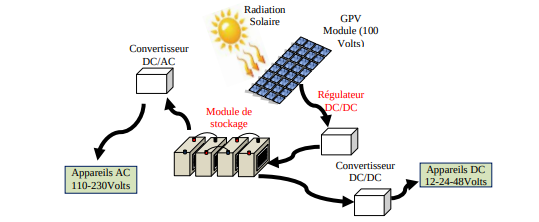
\includegraphics[width=14cm]{./img/standAlone.png}
	\caption{Schéma générale d’une installation PV autonome.}
	\label{i1}
\end{figure}

\begin{figure}[H]
	\centering
	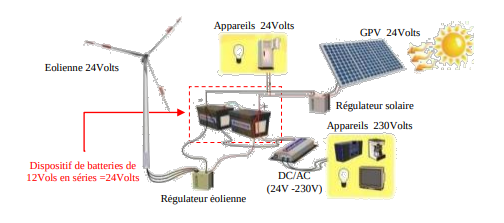
\includegraphics[width=14cm]{./img/hybrid.png}
	\caption{Schéma de raccordement d’une installation Hybride.}
	\label{i1}
\end{figure}


\section{Le panneau photovoltaïque}
Un panneau photovoltaïque est constitué de cellules solaires connectées électriquement en série et/ou en parallèle pour produire le courant et la tension souhaités.

\subsection{Cellule solaire}
La cellule photovoltaïque, fonctionnant grâce à l'effet photovoltaïque découvert par Becquerel en 1839, transforme l'énergie lumineuse en courant électrique via un matériau semi-conducteur, avec une tension d'environ 0,5 à 0,6 V \cite{l3}.\\

Il existe plusieurs types de cellules photovoltaïques :
\begin{itemize}
	\item \textbf{Cellule multi-jonction :} destinée aux applications spatiales, non commercialisée.
	\item \textbf{Cellule en silicium monocristallin :} formée à partir d’un seul cristal de silicium, bleu uniforme.
	\item \textbf{Cellule en silicium polycristallin :} composée de plusieurs cristaux, avec des motifs distincts.
	\item \textbf{Cellule en couche mince CIS/CIGS :} fabriquée à partir de cuivre-indium-sélénium ou gallium.
	\item \textbf{Cellule en silicium amorphe :} projette du silicium sur verre, couleur gris foncé ou marron.
	\item \textbf{Cellule CZTS :} produite avec des minerais non toxiques.
\end{itemize}

%\begin{figure}[H]
%	\centering
%	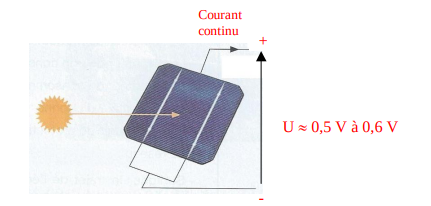
\includegraphics[width=5cm]{./img/cellule.png}
%	\caption{Exemple d'une cellule photovoltaïque}
%	\label{i1}
%\end{figure}
\subsubsection{Principe de fonctionnement}
Prenons le cas d'une cellule photovoltaïque fabriquée à partir de deux couches de silicium (matériau semi-conducteur) :
\begin{itemize}
	\item Une couche dopée avec du bore, qui possède moins d'électrons que le silicium, est dopée positivement (zone P).
	\item Une couche dopée avec du phosphore, qui possède plus d'électrons que le silicium, est dopée négativement (zone N).
\end{itemize}

\begin{figure}[H]
	\centering
	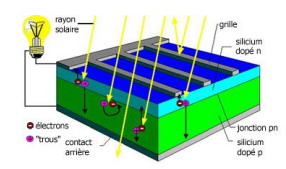
\includegraphics[width=8cm]{./img/cellulePrincipe.png}
	\caption{Détail d'une cellule photovoltaïque}
	\label{i1}
\end{figure}

Lorsqu'un photon de lumière arrive, son énergie crée une rupture entre un atome de silicium et un électron, modifiant les charges électriques. Les atomes, chargés positivement, migrent vers la zone P, tandis que les électrons, chargés négativement, se déplacent vers la zone N. Une différence de potentiel électrique, c'est-à-dire une tension électrique, est ainsi crée. C'est ce qu'on appelle l'effet photovoltaïque.

%\subsubsection{Association des cellules en série}

%Les caractéristiques d’une seule cellule photovoltaïque ne suffisent pas pour alimenter des équipements électriques. Les cellules sont donc associées en série pour obtenir une tension plus élevée, formant un module solaire ou panneau photovoltaïque de 9 ou 12 volts ... La puissance d’un panneau dépend de sa surface et du nombre de cellules qu'il contient.


%\begin{figure}[H]
%	\centering
%	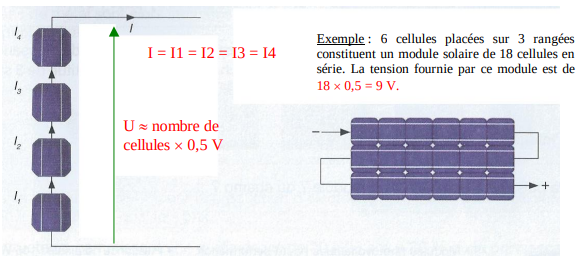
\includegraphics[width=15cm]{./img/exemple.png}
%	\caption{Exemple d'une association des cellules en série}
%	\label{i1}
%\end{figure}

%Pour faire fonctionner des appareils, l’intensité (I) du panneau, variant avec l’ensoleillement, détermine l’énergie produite. La puissance crête d’une installation, exprimée en watt-crête (Wc), est la puissance maximale fournie dans des conditions optimales d’orientation, d’inclinaison et d’ensoleillement.On peut trouver des variété de puissance d'un panneaux solaire comme 50, 100, 150, 200, 280, 300, 340 Wc , ... 

\subsubsection{Constitution d’un champ photovoltaïque}
Les panneaux solaires sont connectés en série pour obtenir la tension nécessaire à l'onduleur, formant une chaîne de modules ou "string". Les chaînes sont ensuite associées en parallèle pour constituer un champ photovoltaïque (champ PV). Des diodes ou des fusibles en série sur chaque chaîne protègent contre les courants inverses causés par l'ombre, évitant ainsi d'endommager les modules.\\

Il existe des differentes types de panneaux solaires :
\begin{itemize}
	\item Monocristallin
	\item Polycristallin
	\item Amorphe
	\item Multi-jonction
	\item CIS et CIGS
	\item CZTS
\end{itemize}
%\begin{figure}[H]
%	\centering
%	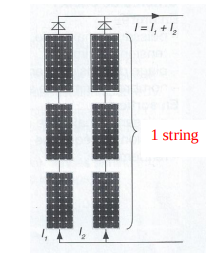
\includegraphics[width=6cm]{./img/string.png}
%	\caption{Chaîne de module ou "String"}
%	\label{i1}
%\end{figure}

%\subsection{Comparaison entre les différents types de panneaux solaires}

%Nous allons voir dans le tableau ci-dessous les différences entre les types de panneaux solaires selon leurs technologies de construction.

%\begin{table}[H]
%	\centering
%	\begin{tabular}{|>{\centering\arraybackslash}m{3cm}|>{\centering\arraybackslash}m{11cm}|>{\centering\arraybackslash}m{1.5cm}|}
%		\hline
%		\textbf{Technologie} & \textbf{Caractéristique} & \textbf{Part de marché} \\			
%		\hline
%		Monocristallin & \begin{itemize}
%			\item Très bon rendement : 14 à 20 \%.
%			\item Durée de vie : importante (30 ans).
%			\item Coût de fabrication : élevé.
%			\item Puissance : 100 à 150 Wc/m\textsuperscript{2}.
%%			\item Rendement faible sous un faible éclairement.
%			\item Perte de rendement avec l’élévation de la température.
%			\item Fabrication : élaborés à partir d’un bloc de silicium fondu qui s’est solidifié en formant un seul cristal.
%			\item Couleur bleue uniforme.
%		\end{itemize} & 43 \% \\
%		\hline
%		Polycristallin & \begin{itemize}
%			\item Bon rendement : 11 à 15 \%.
%			\item Durée de vie : importante (30 ans).
%			\item Coût de fabrication : meilleur marché que les panneaux monocristallins.
%			\item Puissance : 100 Wc/m\textsuperscript{2}.
%			\item Rendement faible sous un faible éclairement.
%			\item Perte de rendement avec l’élévation de la température.
%			\item Fabrication : élaborés à partir de silicium de qualité électronique qui, en se refroidissant, forme plusieurs cristaux.
%			\item Ces cellules sont bleues, mais non uniformes : on distingue des motifs créés par les différents cristaux.
%		\end{itemize} & 47 \%  \\
%		\hline
%		Amorphe & \begin{itemize}
%			\item Rendement faible : 5 à 9 \%.
%			\item Durée de vie : assez importante (20 ans).
%			\item Coût de fabrication : peu onéreux par rapport aux autres technologies.
%			\item Puissance : 50 Wc/m\textsuperscript{2}.
%			\item Fonctionnement correct avec un éclairement faible.
%			\item Peu sensible aux températures élevées.
%			\item Utilisables en panneaux souples.
%			\item Surface de panneaux plus importante que pour les autres panneaux au silicium.
%			\item Rendement faible en plein soleil.
%			\item Performances diminuant avec le temps.
%			\item Fabrication : couches très minces de silicium appliquées sur du verre, du plastique souple ou du métal, par un procédé de vaporisation sous vide.
%		\end{itemize} & 10 \%  \\
%		\hline
%	\end{tabular}
%\end{table}

%\begin{table}[H]%
%	\centering
%	\begin{tabular}{|>{\centering\arraybackslash}m{3cm}|>{\centering\arraybackslash}m{11cm}|>{\centering\arraybackslash}m{1.5cm}|}
%		\hline
		%\textbf{Technologie} & \textbf{Caractéristique} & \textbf{Part de marché} \\			
%		\hline
%		Multi-jonction & \begin{itemize}
%			\item Très haut rendement : 30 à 40 \%.
%			\item Durée de vie : environ 25 ans.
%			\item Coût de fabrication : très élevé.
%			\item Puissance : 200 à 300 Wc/m\textsuperscript{2}.
%			\item Rendement élevé sous faible éclairement et haute température.
%			\item Utilisation : principalement dans les applications spatiales et militaires.
%			\item Fabrication : combinaison de plusieurs matériaux semi-conducteurs pour absorber un spectre large de lumière solaire.
%		\end{itemize} & 1 \%  \\
%		\hline
%		CIS et CIGS & \begin{itemize}
%			\item Bon rendement : 10 à 12 \%.
%			\item Durée de vie : environ 20 à 25 ans.
%			\item Coût de fabrication : modéré.
%			\item Puissance : 80 à 120 Wc/m\textsuperscript{2}.
%			\item Bon rendement sous faible éclairement et haute température.
%			\item Flexibilité : utilisables sur des surfaces courbes.
%			\item Fabrication : couches minces de cuivre, indium, gallium et sélénium appliquées sur un substrat.
%		\end{itemize} & 5 \%  \\
%		\hline
%		CZTS & \begin{itemize}
%			\item Rendement moyen : 7 à 11 \%.
%			\item Durée de vie : environ 20 ans.
%			\item Coût de fabrication : modéré.
%			\item Puissance : 70 à 100 Wc/m\textsuperscript{2}.
%			\item Bon rendement sous faible éclairement.
%			\item Moins sensible aux variations de température.
%			\item Fabrication : couches minces de cuivre, zinc, étain et sulfure appliquées sur un substrat.
%		\end{itemize} & 1 \%  \\
%		\hline
%	\end{tabular}
%	\caption{Comparaison entre les types de panneaux solaires} \vspace{5mm}
%\end{table}
\newpage
\section{Les batteries}
Une batterie d'accumulateurs appelée plus communément batterie est un assemblage d'accumulateurs électrochimiques.
Un accumulateur électrochimique est un "générateur réversible", il peut stocker l'énergie électrique sous forme chimique puis la restituer à tout moment sur demande grâce à la réversibilité de la transformation.

Cette réaction est activée au sein d'une cellule élémentaire entre deux électrodes baignant dans un électrolyte, lorsqu'une charge est branchée à ses bornes.
L'accumulateur est basé sur un système électrochimique réversible et donc rechargeable, contrairement à une pile  .\\

\subsection{Classification des batteries}
Les batteries peuvent être classées en deux grandes catégories : les accumulateurs primaires (non-rechargeables) et les accumulateurs secondaires (rechargeables)\cite{l1}. De plus, il existe d'autres classifications basées soit sur des critères technologiques spécifiques (conception), soit sur des domaines d'utilisation spécifiques.

\begin{itemize}
	\item \textbf{Batteries primaires} : Non rechargeables, utilisées dans les télécommandes et lampes de poche.
	\item \textbf{Batteries secondaires} : Rechargeables, utilisées dans les téléphones, ordinateurs portables et voitures électriques.
\end{itemize}


\subsection{Les paramètres d'une batterie}

Les divers domaines d'utilisation des batteries ont conduit à l'élaboration de plusieurs critères essentiels pour évaluer leur état et leurs performances.

\subsubsection{La tension}

La tension est le voltage aux bornes de la batterie (Vt), un paramètre facilement mesurable. Différentes tensions de référence sont définies :

\begin{itemize}
	\item \textbf{Tension théorique (\(E_{\text{th}}\))} : dépend des matériaux actifs (anode, cathode, électrolyte) et de la température, calculée selon la loi de Nernst.
	\item \textbf{Tension nominale (\(V_{\text{n}}\))} : tension typique recommandée en fonctionnement normal, par exemple, 2.0V pour une cellule plomb-acide.
	\item \textbf{Tension de fin de décharge (\(V_{\text{Cut-Off}}\))} : tension à laquelle la batterie est considérée vide, par exemple, 1.75V pour le plomb-acide et 2.5V pour le Li-ion.
	\item \textbf{Tension de fin de charge (\(V_{\text{full}}\))} : tension à laquelle la batterie est pleinement chargée, par exemple, 2.03V pour le plomb-acide et 4.2V pour le Li-ion.
	\item \textbf{Tension à circuit ouvert (\(V_{\text{OC}}\))} : tension mesurée sans charge, liée à l'état de charge (SOC). Elle nécessite un temps de relaxation après charge/décharge pour des mesures précises.
\end{itemize}
\paragraph{La tension de charge :}
Il existe plusieurs tensions de charge à respecter selon les différents stades de recharge de la batterie. Les batteries au plomb-acide, y compris les batteries Gel et AGM, suivent les étapes suivantes pendant la charge. Prenons le cas d'une batterie avec une tension nominale de 12V :

\begin{itemize}
	\item \textbf{Étape de Bulk (Charge en vrac)} :
	lors de la première phase de charge, la batterie est chargée à un courant maximum, avec une tension qui augmente progressivement jusqu'à environ 14.4V, permettant de recharger rapidement 70 à 80\% de sa capacité totale. Cette phase, la plus longue, fournit la majorité de la charge.
	
	\item \textbf{Étape d'Absorption} :
	la tension est maintenue constante à 14.4V tandis que le courant diminue progressivement, permettant de compléter les 20 à 30\% restants de la charge sans surcharger la batterie. Cette phase se poursuit jusqu'à ce que le courant devienne très faible, indiquant que la batterie est presque entièrement chargée.
	
	\item \textbf{Étape de Float (Maintien de charge ou charge de maintien)} :
	la tension est réduite à 13.5V à 13.8V pour maintenir la batterie en pleine charge sans l'endommager, en compensant l'auto-décharge avec un courant très faible. Cette phase peut être maintenue indéfiniment tant que la batterie reste connectée, garantissant qu'elle est toujours prête à l'emploi.
\end{itemize}

D'autres types de batteries utilisent également leur propre processus de charge.


\begin{figure}[H]
	\centering
	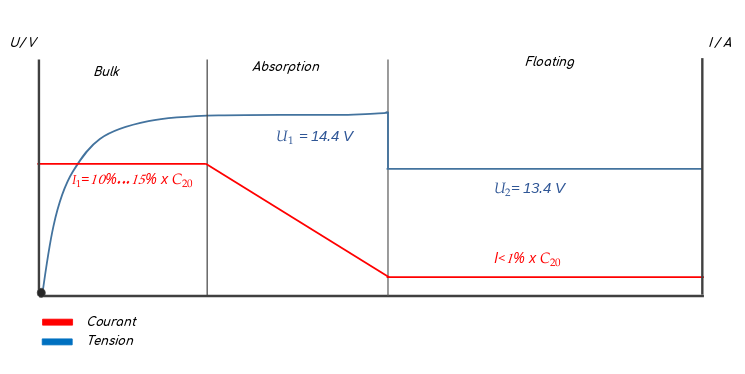
\includegraphics[width=16cm]{./img/ChargebatHumide.png}
	\caption{Les étapes de la tension de charge }
	\label{i1}
\end{figure}


\subsubsection{Le courant}

Le courant est la quantité de charge électrique qui circule à travers la batterie par unité de temps, mesurée en ampères (A). Plusieurs types de courants sont importants pour évaluer les performances et le comportement d'une batterie :

\begin{itemize}
	\item \textbf{Courant de charge (\(I_{\text{charge}}\))} : le courant appliqué à la batterie lors de son chargement. Il est souvent exprimé en fonction de la capacité nominale de la batterie (C), par exemple, un courant de charge de 0.1C pour une batterie de 100Ah serait de 10A.
	\item \textbf{Courant de décharge (\(I_{\text{discharge}}\))} : le courant que la batterie délivre lors de son utilisation. Comme pour le courant de charge, il est souvent exprimé en multiples de la capacité (C), par exemple, un courant de décharge de 0.5C pour une batterie de 100Ah serait de 50A.
	\item \textbf{Courant de pointe (\(I_{\text{peak}}\))} : le maximum de courant que la batterie peut fournir sur de courtes périodes sans subir de dommages. Ce paramètre est crucial pour des applications nécessitant des pics de puissance élevés.
	\item \textbf{Courant de repos (\(I_{\text{rest}}\))} : le courant minimal que la batterie délivre ou reçoit lorsqu'elle est en état de repos ou en charge très faible. Il est important pour évaluer les pertes internes de la batterie.
	\item \textbf{Courant de court-circuit (\(I_{\text{sc}}\))} : le courant maximal que la batterie peut fournir en cas de court-circuit. Il dépend de la résistance interne de la batterie et est un paramètre important pour la sécurité.
\end{itemize}

\subsubsection{La température}

Les températures extrêmes, qu'elles soient très élevées ou très basses, peuvent considérablement affecter le fonctionnement d'une batterie en service, influençant ainsi ses performances et d'autres paramètres critiques.

\subsubsection{La capacité}

\begin{itemize}
	\item \textbf{Capacité massique} : rapport entre l'énergie disponible d'une batterie ou cellule et son poids, exprimée en Wh/kg.
	\item \textbf{Capacité nominale (CN)} : valeur de la capacité indiquée par le fabricant pour des conditions d'opération spécifiques (température définie, courant et tension de coupure).
	\item \textbf{	C-rate (nC)} : mesure le courant de charge ou de décharge d'une batterie par rapport à sa capacité nominale. Une batterie évaluée à 1C fournit un courant égal à sa capacité en ampères pendant une heure. Par exemple, une batterie de 1000mAh à 1C fournit 1A pendant une heure, à 0.5C fournit 500mA pendant 2 heures, et à 2C fournit 2A pendant 30 minutes.
\end{itemize}

\subsubsection{Phénomène d'autodécharge}
L'autodécharge est la décomposition spontanée des matériaux actifs d'une cellule, entraînant une perte d'EMF due à une fuite interne de courant. Les batteries primaires sont les moins sujettes à l'autodécharge, suivies des batteries secondaires (rechargeables).

\begin{table}[h!]
	\centering
	\begin{tabular}{|>{\centering\arraybackslash}m{3cm}|>{\centering\arraybackslash}m{13cm}|}
		\hline
			\rule[0.5cm]{0cm}{0cm}\textbf{Type de batteries} & \textbf{Estimation de l'autodécharge} \\ \hline
			\rule[0.5cm]{0cm}{0cm}Primaire & 10\% en 5 ans\\ \hline
			\rule[0.5cm]{0cm}{0cm}Plomb-acide& 5\% par mois\\ \hline
		\rule[0.5cm]{0cm}{0cm}	Ni-Cd & 10-15\% en 24 heures, puis 10-15\% par 	\rule[0.5cm]{0cm}{0cm}mois \\ \hline
			\rule[0.5cm]{0cm}{0cm}Ni-MH & 30\% (avec faible résistance et grande capacité massique) \\ \hline
			\rule[0.5cm]{0cm}{0cm}Li-Ion& 5\% en 24 heures, puis 1-2\% /mois, >3\% pour les circuits de protection \\ \hline
	\end{tabular}
	\caption{Estimation de l'autodécharge pour différents types de batteries}
	\label{tab:autodecharge}
\end{table}

\newpage
\subsubsection{État de Charge (SoC)}
L'état de charge (SoC) d'une batterie représente l'énergie restante, influencé par des facteurs comme le courant et la température. Exprimé en pourcentage, 100\% indique une batterie pleine, et 0\% une batterie vide. Le SoC peut être déterminé par la méthode de comptage de Coulombs \cite{a1} \cite{a2} \cite{l2}.


\begin{equation}
\text{SoC}(t) = \text{SoC}(t-1) + \frac{1}{C_{\text{n}}} \int_{t-1}^{t} i(t) \, dt
\end{equation}

où :

\begin{itemize}
	\item \(\text{SoC}(t)\) est l'état de charge au temps \(t\),
	\item \(\text{SoC}(t-1)\) est l'état de charge au temps \(t-1\),
	\item \(i(\tau)\) est le courant mesuré à l'instant \(\tau\),
	\item \(C_{\text{n}}\) est la capacité nominale de la batterie en ampères-heures (Ah),
\end{itemize}

En pratique, la capacité actuelle (\(Q\)) peut être calculée à partir de la somme des produits du courant (\(I\)) et du temps (\(\Delta t\)) pour chaque intervalle de mesure :

\begin{equation}
Q = \int_{t_0}^{t} i(t) \, dt
\end{equation}

En pratique, cette intégration est souvent effectuée de manière discrète :

\begin{equation}
Q = \sum_{i=0}^{n} I_i \Delta t_i
\end{equation}

où :

\begin{itemize}
	\item \(I_i\) est le courant mesuré à l'intervalle \(i\),
	\item \(\Delta t_i\) est la durée de l'intervalle \(i\).
\end{itemize}

\subsubsection{La Profondeur de Décharge (DoD)}
La profondeur de décharge (DoD) indique la capacité retirée d'une batterie lors d'un cycle de décharge, exprimée en pourcentage par rapport à sa capacité maximale \cite{a2}. Par exemple, pour une batterie « YUASA 12V-24Ah », la DoD est calculée lorsque la batterie est déchargée avec un courant de 1,23A jusqu'à 12Ah de sa capacité C20.

\begin{equation}
\text{DoD} \% = \left( \frac{\text{Capacité retirée d'une batterie chargée (Ah)}}{C_x (\text{Ah})} \right) \times 100
\end{equation}

D'après cette équation  :

\[
\text{DoD} = \left( \frac{\text{Capacité initiale} - \text{Capacité retirée}}{C_{20}} \right) \times 100
\]

\[
\left( \frac{24\text{Ah} - 12\text{Ah}}{24\text{Ah}} \right) \times 100 = 50\%
\]

Selon ces équations , la profondeur de décharge est le complément de l'état de charge (SoC) :
\begin{equation}
\text{DoD} \% = (1 - \text{SoC}) \times 100
\end{equation}

Ce paramètre est crucial pour le dimensionnement correct d'une batterie. Identifier précisément la DoD permet de gérer efficacement la durée de vie et la performance de la batterie.

\subsubsection{Le Nombre de Cycles (Nb\_Cycles)}
Le nombre de cycles (Nb\_Cycles) correspond au nombre de cycles charge/décharge qu'une batterie peut effectuer tout en maintenant sa tension de coupure au-dessus de V\textsubscript{Cut-Off}. Il dépend de la profondeur de décharge (DoD) et est généralement fourni par le fabricant, mais peut être déterminé après des tests spécifiques. Ce paramètre influence la durée de vie et la performance de la batterie.

\subsubsection{L’état de santé (SOH)}
L’état de santé (SOH) mesure la capacité de la batterie à fournir les performances spécifiées par rapport à une batterie neuve. Il permet d’estimer la durée de vie restante (Nb\_Cycles) et suit la dégradation des performances \cite{a2}.


\begin{equation}
\text{SOH} \% = \left( \frac{\text{Capacité d'une batterie utilisée (Ah)}}{C_x (\text{Ah})} \right) \times 100
\end{equation}

Pour certaines prédéfinitions, la batterie est considérée en fin de vie (EOL) lorsqu'elle atteint un SOH de 80\%. Cela signifie que lorsqu'une batterie ne peut plus fournir que 80\% de sa capacité nominale, elle doit être remplacée ou reconditionnée pour continuer à garantir des performances optimales.

\subsection{Structure de la batterie}
Une batterie est constituée de plusieurs cellules électrochimiques assemblées en structures prismatiques, cylindriques, etc. Ces cellules forment la batterie, définissant sa tension, son courant, et sa durée de vie, selon les normes ou l'application.


\begin{figure}[H]
	\centering
	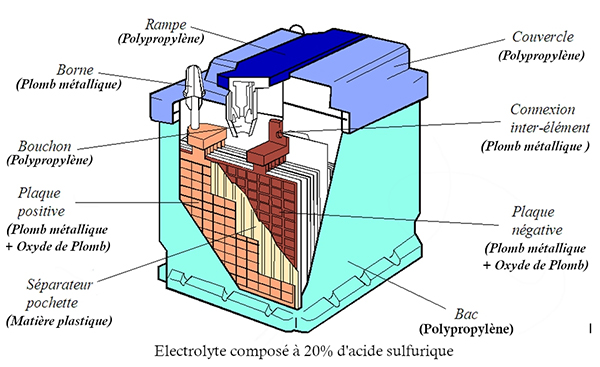
\includegraphics[width=13cm]{./img/stricture1.jpg}
	\caption{Structure d'une batterie}
	\label{i1}
\end{figure}
\subsection{Les batteries solaires}

Les batteries solaires stockent l'énergie produite par les panneaux photovoltaïques. Elles sont essentielles pour les systèmes autonomes, car les panneaux ne génèrent de l'électricité que durant la journée. Les batteries permettent d'utiliser l'électricité stockée pendant la nuit ou par temps nuageux.

\subsubsection{Fonctionnement d’une batterie solaire}

Les batteries solaires stockent l'énergie sous forme chimique et la libèrent via des réactions internes. Conçues pour des décharges lentes et des recharges espacées, elles accumulent plus d’énergie que les batteries de voiture ou d’appareils électroniques.


\subsection{Types de Batteries Solaires}

Les batteries solaires se classifient en plusieurs types, chacun ayant ses caractéristiques spécifiques. Voici les principales catégories \cite{a3} \cite{a4} :

\begin{table}[h!]
	\centering
	\begin{tabular}{|>{\centering\arraybackslash}m{5cm}|>{\centering\arraybackslash}m{10cm}|}
		\hline
		\textbf{Type de Batterie} & \textbf{Exemples} \\ \hline
		\rule[0.5cm]{0cm}{0cm} \textbf{Batteries au Plomb} & Plomb Acide Liquide (Inondées ou Plomb Ouvert), AGM, Gel \\ \hline
		\rule[0.5cm]{0cm}{0cm} \textbf{Batteries au Lithium} & Lithium-Ion, LiFePO4, LiMn2O4 \\ \hline
		\rule[0.5cm]{0cm}{0cm} \textbf{Autres Technologies} & Batteries à Flux (Redox), Batteries à Électrolyte Solide, Batteries Zinc-Air, Batteries Aluminium-Air \\ \hline
	\end{tabular}
	\caption{Types de batteries et leurs exemples}
\end{table}
	

Bien que d'autres types de batteries existent, ceux mentionnés ci-dessus sont fréquemment utilisés et disponibles sur le marché.

Chaque type de batterie a ses propres tensions de charge et décharge spécifiques. Examinons les tensions de charge pour différentes batteries ayant une tension nominale de 12V :


\begin{table}[h!]
	\centering
	\begin{tabular}{|>{\centering\arraybackslash}m{5cm}|>{\centering\arraybackslash}m{5cm}|>{\centering\arraybackslash}m{5cm}|}
		\hline
			\rule[0.5cm]{0cm}{0cm}\textbf{Type de Batterie} &	\rule[0.5cm]{0cm}{0cm} \textbf{Tension de Charge Maximale} & \textbf{Tension de Décharge Minimale} \\ \hline

			\rule[0.5cm]{0cm}{0cm}\quad  Plomb Acide  & 14.4V - 14.8V & 10.5V \\ \hline
			\rule[0.5cm]{0cm}{0cm}\quad  AGM  & 14.4V - 14.6V & 10.5V \\ \hline
			\rule[0.5cm]{0cm}{0cm}\quad   Gel & 14.2V - 14.4V & 10.5V \\ \hline
	
		\rule[0.5cm]{0cm}{0cm}	\quad  Lithium-Ion & 4.2V par cellule & 2.5V - 3.0V par cellule \\ \hline
		\rule[0.5cm]{0cm}{0cm}	\quad  LiFePO4 & 3.6V - 3.65V par cellule & 2.0V - 2.5V par cellule \\ \hline
			\rule[0.5cm]{0cm}{0cm}\quad  LiMn2O4 & 4.2V par cellule & 2.5V - 3.0V par cellule \\ \hline
	\end{tabular}
	\caption{Tensions de charge maximales et de décharge minimales}
\end{table}



\subsubsection{Comparaison des Types de Batteries Solaires}

Le tableau ci-dessous présente une comparaison des différents types de batteries solaires, mettant en évidence leurs caractéristiques distinctes et leurs différences :

\begin{landscape}
	\begin{table}[h!]
		\centering
		\caption{Comparaison des différents types de batteries solaires}\vspace{0.3cm}
		\begin{tabular}{|>{\centering\arraybackslash}m{3cm}|>{\centering\arraybackslash}m{1.5cm}|>{\centering\arraybackslash}m{1.5cm}|>{\centering\arraybackslash}m{3cm}|>{\centering\arraybackslash}m{2cm}|>{\centering\arraybackslash}m{5cm}|>{\centering\arraybackslash}m{3cm}|>{\centering\arraybackslash}m{1.5cm}|}
			\hline
				\rule[0.5cm]{0cm}{0cm}\textbf{Type de Batterie} & \textbf{Cycles de Vie} & \textbf{DoD (\%)} & \textbf{Matériaux} & \textbf{Prix} & \textbf{Impact Environnemental} & \textbf{Température (\textdegree C)} & \textbf{Volume} \\
			\hline
			Plomb Acide Liquide & 500-1000 & 50-70 & Plomb, acide sulfurique & Moins cher & Pollution par le plomb, recyclage possible, dégage de l'hydrogène & -20 à 50 & Grand \\
			\hline
			AGM  & 600-1200 & 60-80 & Plomb, acide sulfurique & Moins cher & Pollution par le plomb, recyclage possible, dégage de l'hydrogène & -20 à 50 & Moyen \\
			\hline
			Gel & 700-1400 & 60-80 & Plomb, électrolyte gélifié & Modéré & Pollution par le plomb, recyclage possible, dégage de l'hydrogène & -20 à 50 & Moyen \\
			\hline
			Lithium-Ion & 2000-5000 & 80-90 & Lithium, cobalt, nickel & Cher & Extraction de lithium, recyclage complexe, dégage de la chaleur & -20 à 60 & Petit \\
			\hline
			Lithium-Fer-Phosphate (LiFePO4) & 3000-7000 & 80-90 & Lithium, fer, phosphate & Modéré & Impact moindre, recyclage possible, dégage de la chaleur & -20 à 60 & Petit \\
			\hline
			Lithium-Manganèse (LiMn2O4) & 1000-2000 & 80-90 & Lithium, manganèse & Modéré & Extraction de lithium et manganèse, recyclage complexe, dégage de la chaleur & -20 à 60 & Petit \\
			\hline
			Batteries à Flux (Redox) & 5000-10000 & 100 & Vanadium, électrolytes liquides & Modéré & Impact limité, électrolytes recyclables, peut dégrader l'environnement aqueux & -10 à 40 & Très grand \\
			\hline
			Batteries à Électrolyte Solide & 1000-5000 & 80-90 & Matériaux solides, lithium & Cher & Impact limité, recyclage complexe, dégage de la chaleur & -20 à 60 & Petit à moyen \\
			\hline
			Batteries Zinc-Air & 200-500 & 100 & Zinc, air & Moins cher & Impact faible, recyclable, dégage de l'oxygène & -20 à 50 & Moyen \\
			\hline
			Batteries Aluminium-Air & 200-500 & 100 & Aluminium, air & Moins cher & Impact faible, recyclable, dégage de l'oxygène & -20 à 50 & Moyen à grand \\
			\hline
		\end{tabular}
	\end{table}
\end{landscape}

%\subsection{Réactions chimiques pendant la charge et décharge}
%Comprendre les phénomènes chimiques fondamentaux est crucial pour appréhender le fonctionnement des batteries. Nous allons examiner les réactions chimiques typiques qui se produisent pendant la charge et la décharge dans deux types de batteries : les batteries au plomb et les batteries au lithium \cite{t1}.
%
%\subsubsection{La batterie au Plomb-Acide}
%
%La batterie au plomb-acide est une technologie largement éprouvée et presque entièrement recyclable. Elle se distingue par son coût relativement bas par rapport aux autres types de batteries, ce qui en fait une référence pour comparer les performances des autres technologies. Son principe de fonctionnement repose sur une réaction d'oxydoréduction caractéristique :
%
%\[
%\text{PbO}_2 + \text{Pb} + 2 \text{H}_2\text{SO}_4 \rightleftharpoons 2 \text{PbSO}_4 + 2 \text{H}_2\text{O}
%\]
%
%Ici, \(\text{PbO}_2\) est l'électrode positive (+) et \(\text{Pb}\) est l'électrode négative (-). L'électrolyte utilisé est l'acide sulfurique (\(\text{H}_2\text{SO}_4\)).\\
%
%\textbf{Processus de décharge :}
%Pendant la décharge, le plomb à l'anode s'oxyde en perdant deux électrons, tandis que le plomb à la cathode se réduit en gagnant deux électrons. L'hydrogène et l'oxygène formés se combinent pour créer de l'eau (\(\text{H}_2\text{O}\)).
%	\begin{align*}
%	\textbf{Anode (-)} &: \text{Pb} + \text{H}_2\text{SO}_4 \rightarrow \text{PbSO}_4 + 2 \text{H}^+ + 2 e^-\\
%	\textbf{Cathode (+) }&:\text{PbO}_2 + \text{H}_2\text{SO}_4 + 2 e^- \rightarrow \text{PbSO}_4 + 2 \text{OH}^-\\
%	\textbf{Cellule} &:\text{PbO}_2 + \text{Pb} + 2 \text{H}_2\text{SO}_4 \rightleftharpoons 2 \text{PbSO}_4 + 2 \text{H}_2\text{O}
%	\end{align*}
%
%
%\textbf{Processus de charge :}
%Lors de la charge, les réactions inverses de celles de la décharge se produisent, car ces réactions sont réversibles. L'eau est décomposée aux électrodes, l'oxygène réagit avec le plomb à l'électrode positive, tandis que l'hydrogène réagit avec l'acide à l'électrode négative.
%\begin{align*}
%	\textbf{Anode (+)} & : \text{Pb}^{2+} + 2 \text{H}_2\text{O} \rightarrow \text{PbO}_2 + 4 \text{H}^+ + 2 e^- \\
%	\textbf{Cathode (-)} &: \text{PbSO}_4 + 2 e^- \rightarrow \text{Pb} + \text{SO}_4^{2-} \\
%	\textbf{Cellule} &:\text{Pb}^{2+} + 2 \text{H}_2\text{O} \rightleftharpoons \text{PbO}_2 + \text{Pb} + 4 \text{H}^+ 
%\end{align*}
%
%
%\subsubsection{La batterie lithium-ion (Li-Ion) :}
%Grâce à ses caractéristiques attrayantes, comme la légèreté du lithium (6,94 g/mol) et sa densité énergétique élevée (3860 mAh/g), cette technologie a été étudiée depuis les années 1950. Les premières batteries commerciales Li-Ion sont apparues dans les années 1990. Aujourd'hui, les types les plus courants sont les Lithium-Ion (Li-Ion) et Lithium-Polymères (Li-Po).
%
%\textbf{Processus de décharge} :
%Pendant la décharge, les ions lithium (\(\text{Li}^+\)) se déplacent de l'anode (négative) vers l'électrolyte, tandis que les électrons (\(e^-\)) circulent dans le circuit externe pour fournir de l'énergie. À la cathode (positive), les ions lithium et les électrons réagissent avec \(\text{Li}_{1-x}\text{CoO}_2\) pour former \(\text{LiCoO}_2\). Cette réaction maintient l'équilibre entre les états chargés et déchargés des matériaux actifs.
%\begin{align*}
%\text{Anode (-)} & : \text{Li}_x\text{C} \rightarrow \text{C} + x \text{Li}^+ + x e^-  \\
%\text{Cathode (+)} & : \text{Li}_{1-x}\text{CoO}_2 + x \text{Li}^+ + x e^- \rightarrow \text{LiCoO}_2 \\
%\text{CELLULE} & : \text{Li}_{1-x}\text{CoO}_2 + \text{Li}_x\text{C} \leftrightarrows \text{C} + \text{LiCoO}_2 
%\end{align*}
%
%\textbf{Processus de charge} :
%es électrons (\(e^-\)) sont extraits de l'anode (positive) par une source d'alimentation externe et passent par le circuit externe. Simultanément, les ions lithium (\(\text{Li}^+\)) migrent de la cathode (négative) vers l'anode à travers l'électrolyte. À l'anode, les ions lithium se réintègrent dans le graphite pour reformer \(\text{Li}_x\text{C}\). À la cathode, les électrons et les ions lithium réagissent pour reformer \(\text{Li}_{1-x}\text{CoO}_2\). Ce processus recharge les matériaux actifs de la batterie.
%\begin{align*}
%\text{Anode (+)} & : \text{LiCoO}_2 \rightarrow \text{Li}_{1-x}\text{CoO}_2 + x \text{Li}^+ + x e^-  \\
%\text{Cathode (-)} & : \text{C} + x \text{Li}^+ + x e^- \rightarrow \text{Li}_x\text{C}  \\
%\text{CELLULE} & : \text{Li}_{1-x}\text{CoO}_2 + \text{Li}_x\text{C} \leftrightarrows \text{C} + \text{LiCoO}_2 
%\end{align*}

\section{Procédure de dimensionnement d’une champ photovoltaïque }
La conception d'une installation photovoltaïque autonome est un processus assez complexe en raison des nombreux paramètres à prendre en compte.

\subsection{Besoin énergétique des applications}

Pour dimensionner correctement un système, il est crucial d'évaluer les besoins énergétiques des applications à alimenter, ce qui se traduit par la puissance nécessaire. La relation entre puissance et énergie, deux grandeurs liées par le temps, est donnée par :
\begin{figure}[H]
	\centering
	\begin{subfigure}{0.40\textwidth} % Largeur de la partie formule
		\centering
		\begin{equation}
		E = P \times t
		\end{equation}
	\end{subfigure}
	\hfill
	\begin{subfigure}{0.55\textwidth} % Largeur de la partie explication
		\centering
		\begin{itemize}
			\item \( E \) : énergie (en Wh/j),
			\item \( P \) : puissance (en Watts),
			\item \( t \) : temps d’utilisation (en heures).
		\end{itemize}
	\end{subfigure}
\end{figure}


Cette formule permet de calculer le besoin énergétique journalier d'une application, en multipliant la puissance consommée par la durée d’utilisation quotidienne.

\subsection{Énergie solaire récupérable}

\subsubsection{Inclinaison et orientation des panneaux}  
L'orientation et l'inclinaison des panneaux influencent directement leur rendement. Pour maximiser la production, ils doivent être orientés vers l'équateur (sud dans l'hémisphère nord, nord dans l'hémisphère sud) et inclinés selon la période la moins ensoleillée.  

\subsubsection{Données météorologiques}  
Le dimensionnement photovoltaïque dépend du rayonnement solaire local : plus il est élevé, moins il faut de panneaux pour un besoin donné.

\subsection{Énergie produite (Wh/jour)}

L'énergie à produire par le champ photovoltaïque est calculée selon la formule suivante :

\begin{equation}
Ep \, (\text{Wh}) = \frac{Ec}{k}
\end{equation}

Où :

\begin{itemize}
	\item \textbf{Ep} : Énergie à produire par le champ photovoltaïque en Wh/jour
	\item \textbf{Ec} : Énergie totale consommée en Wh/jour
\item \textbf{k} : Facteur de correction tenant compte des incertitudes météorologiques, du rendement des modules, des batteries, du régulateur, de l'onduleur et des pertes dans les câbles. Il varie entre 0,55 et 0,75.

\end{itemize}

\subsection{Puissance crête (Pc) des modules photovoltaïques}

La puissance crête totale du champ photovoltaïque dépend de l'irradiation quotidienne du lieu d'utilisation. Elle est donnée par :

\begin{equation}
Pc = \frac{Ep}{Ir}
\end{equation}
Où :

\begin{itemize}
	\item \textbf{Pc} : Puissance crête totale des modules photovoltaïques en W
	\item \textbf{Ep} : Énergie à produire par le champ photovoltaïque en Wh/jour
	\item \textbf{Ir} : Irradiation journalière du mois le plus défavorable en kWh/m²/jour
\end{itemize}

\subsection{Choix de la tension de fonctionnement}

Le choix de la tension de fonctionnement d'un système dépend de la disponibilité du matériel, ainsi que des niveaux de puissance et d'énergie nécessaires selon le type d'application. Le tableau suivant montre les tensions du système correspondant à chaque intervalle de puissance crête :

\begin{table}[H]
	\centering
	\begin{tabular}{|c|c|c|c|c|}
		\hline
			\rule[0.5cm]{0cm}{0cm}\textbf{Puissance du Champ (Wc)} & 0-500 Wc & 500 Wc - 2 kWc  & 2 - 10 kWc & 	> 10 kWc \\
		\hline
			\rule[0.5cm]{0cm}{0cm}\textbf{Tension Recommandée (V DC)} & 12 V  & 24 V & 48 V & > 48 V \\
		\hline
	\end{tabular}
\caption{Tension recommandée pour les systèmes photovoltaïques}
\end{table}

\subsubsection{Choix du type de module photovoltaïque}

Le choix du type de module dépend de plusieurs facteurs : la tension de fonctionnement choisie, la puissance maximale, le courant de court-circuit (Icc), le dimensionnement, et le prix.

\subsubsection{Détermination du nombre de modules à installer}

À partir de la puissance crête des panneaux, le nombre de panneaux solaires nécessaires à l'installation est déterminé par la formule :

\begin{equation}
Np = \frac{Pc}{Ppv}
\end{equation}


Où :

\begin{itemize}
	\item \textbf{Np} : Nombre de panneaux nécessaires
	\item \textbf{Pc} : Puissance crête totale des modules photovoltaïques en W
	\item \textbf{Ppv} : Puissance crête d’un module photovoltaïque en W
\end{itemize}

\subsubsection{Répartition des modules}

Le choix de la tension du générateur PV est étroitement lié à la puissance crête demandée. 
\textbf{Nombre de panneaux en série et en parallèle}\\

\textbf{Nombre de panneaux en série} :
	\begin{equation}
N_s = \frac{U}{U_n}
\end{equation}
Où :
	\begin{itemize}
	\item \textbf{U} : Tension du système,
	\item \textbf{U\textsubscript{n}} : Tension nominale d'un module.
\end{itemize}


\textbf{Nombre de branches en parallèle} :

	\begin{equation}
N_{bp} = \frac{N_{mb}}{N_s}
\end{equation}
Où : 

	\begin{itemize}
	\item \textbf{Nmb} : Nombre total de modules,
	\item \textbf{Ns} : Nombre de panneaux en série.
\end{itemize}


\subsection{Caractéristiques du générateur}

\textbf{Puissance crête d’un champ} :

	\begin{equation}
Pc/champ = N_{bp} \times N_s \times P_{cm}
\end{equation}

Où :
	\begin{itemize}
	\item \textbf{Pcm} : Puissance crête d’un module,
	\item \textbf{Nbp} : Nombre de branches parallèles,
	\item \textbf{Ns} : Nombre de panneaux en série.
\end{itemize}

\textbf{Surface occupée par le générateur} :
	\begin{equation}
St = Sm \times Nm
\end{equation}
Où :
	\begin{itemize}
	\item \textbf{Sm} : Surface d’un module,
	\item \textbf{Nm} : Nombre de modules.
\end{itemize}


\subsection{Dimensionnement des éléments de stockage}

La capacité nominale des batteries est donnée par l’expression :


\begin{equation}
Cu = \frac{Cj \times Nj}{U \times Pd}
\end{equation}
Où :\begin{itemize}
	\item \textbf{Cj} : Capacité journalière requise par champ (en Ah/jour)
	\item \textbf{Nj} : Nombre de jours d'autonomie
	\item \textbf{Pd} : Profondeur de décharge (par exemple, 0.8 pour 80\%).
	\item \textbf{U} : Tension du système (en volts, V)
\end{itemize}
La Capacité Journalière est donnée par :
	\begin{equation}
C_j = \frac{E_j}{U}
\end{equation}


\textbf{Où :}

\begin{itemize}
	\item $C_j$ : Capacité journalière requise par champ (en Ah/jour)
	\item $E_j$ : Énergie journalière nécessaire (en watt-heures, Wh/jour)
	\item $U$ : Tension du système (en volts, V)
\end{itemize}


Autonomie souhaitée pour l'installation : 

\begin{equation}
Estockage = Ep \times Nj
\end{equation}
Où :

\begin{itemize}
	\item \textbf{Estockage} : Énergie de stocker 
	\item \textbf{Nj} : Nombre de jours d'autonomie

\end{itemize}

On détermine le nombre des batteries nécessaire en utilisant les formule suivantes : 
\textbf{Nombre de batteries en série} :
\begin{equation}
N_s = \frac{V_{module}}{V_{batterie}} 
\end{equation}


\textbf{Nombre de chaînes en parallèle} : 

	\begin{equation}
N_p = \frac{Cu}{Cn}
\end{equation}
Où :
	\begin{itemize}
	\item \textbf{Cu} : Capacité totale requise des batteries,
	\item \textbf{Cn} : Capacité nominale d'une seule batterie.
\end{itemize}

\textbf{Nombre total de batteries} :
	\begin{equation}
N_t = N_s \times N_p 
\end{equation}




\subsection{Dimensionnement du régulateur}

Le régulateur contrôle les flux d’énergie et protège la batterie contre les surcharges et décharges profondes. Le régulateur sera dimensionné d’après la tension et le courant d’entrée :

\begin{equation}
Imax = \frac{Pc/champ}{U}
\end{equation}
\subsection{Dimensionnement de l’onduleur}
L'onduleur convertit le courant continu en courant alternatif. Son dimensionnement se base sur la somme des puissances maximales des équipements à alimenter, en tenant compte des courants de pointe élevés et du facteur de puissance (cos \(\theta\)). La puissance apparente (S) est calculée par :

	\begin{equation}
S^2 = P^2 + Q^2
\end{equation}
Où :
	\begin{itemize}
	\item \textbf{P} : Puissance active,
	\item \textbf{Q} : Puissance réactive.
\end{itemize}

\subsection{Choix des câbles}

Les câbles solaires doivent résister aux conditions spéciales liées à leur utilisation. La résistance d’un câble dépend de la résistivité des matériaux, de la longueur du câble, de la section et de la température.

\begin{equation}
R = \frac{\rho \cdot L}{S}
\end{equation}
Où :
	\begin{itemize}
	\item \textbf{R} : Résistance (\(\Omega\)),
	\item \textbf{\(\rho\)} : Résistivité (\(\Omega \cdot\)m),
	\item \textbf{L} : Longueur du câble (m),
	\item \textbf{S} : Section du câble (m²).
\end{itemize}



\subsubsection{Calcul de la section des câbles}

\textbf{Courant de Sortie d’un Panneau} :

	\begin{equation}
I = \frac{P}{U}
\end{equation}
Où :
	\begin{itemize}
	\item \textbf{I} : Courant de sortie d’un panneau en ampère (A),
	\item \textbf{P} : Puissance d’un panneau en watt (W),
	\item \textbf{U} : Tension nominale d’un panneau en volt (V).
\end{itemize}

\textbf{Section des conducteurs entre les panneaux et le boîtier de raccordement} :

\begin{align*}
\Delta U &= U \cdot 0{,}02 & \quad R &= \frac{\Delta U}{I} & \quad S &= \frac{\rho \cdot L}{R}
\end{align*}
\subsection{Courant circulant entre les batteries et l’onduleur}

\textbf{Puissance crête du champ photovoltaïque} :
\begin{align}
Pc &= N \times P & \quad I &= \frac{Pc}{U}
\end{align}


\textbf{Courant circulant entre les batteries et l’onduleur à la puissance nominale} :

\begin{equation}
Imax \, batteries = \frac{P \, max \, onduleur}{U \, batterie}
\end{equation}

\section{Conclusion}
Nous avons étudié les diverses applications des systèmes photovoltaïques et constaté que leur performance dépend de plusieurs facteurs, tels que la qualité des panneaux solaires, des batteries, et des autres équipements utilisés, ainsi que du dimensionnement adéquat du système. Le bon fonctionnement d'une batterie dépend de plusieurs paramètres, notamment la température, la tension et le courant, ce qui nécessite une surveillance régulière afin de garantir des performances optimales.

Dans le chapitre suivant, nous traiterons du fonctionnement des dispositifs de surveillance de ces accumulateurs, indispensables pour optimiser la gestion et la performance des installations photovoltaïques.








	%\chapter*{Introduction générale}
\phantomsection
\addcontentsline{toc}{chapter}{Introduction générale}  

La surveillance des batteries solaires est devenue une nécessité incontournable dans la gestion moderne des systèmes photovoltaïques. Depuis l'émergence des technologies solaires, le besoin de stocker l'énergie produite pour une utilisation ultérieure a conduit à d’importantes avancées dans la conception et la gestion des batteries. Ces systèmes de stockage jouent un rôle essentiel en assurant un approvisionnement énergétique constant, même en l’absence de production solaire.  


Au fil des années, diverses techniques et outils ont été développés pour améliorer la gestion des batteries solaires, notamment grâce à la surveillance en temps réel de leurs paramètres clés. Ces progrès résultent d’efforts continus pour mieux comprendre et optimiser le fonctionnement des batteries, en intégrant des solutions technologiques avancées permettant de mesurer la tension, le courant, la température ainsi que les états de charge et de décharge.  


Bien que les installations solaires se multiplient, la gestion efficace des batteries demeure un défi majeur. Il est crucial de disposer de systèmes de monitoring capables de fournir des données précises et en temps réel afin de maximiser leur durée de vie et garantir des performances optimales. Cela implique une analyse détaillée des courants de charge et de décharge ainsi qu’une surveillance rigoureuse des tensions pour prévenir les défaillances.  


C’est dans ce contexte que ce livre explore les principes fondamentaux du monitoring des batteries solaires. Il débute par une vue d’ensemble des systèmes photovoltaïques et des batteries, en détaillant leurs principes de fonctionnement et caractéristiques. Ensuite, il traite des composants électroniques dédiés à la surveillance et examine les techniques de transmission des données en temps réel ainsi que la modélisation des bases de données, essentielles pour une gestion efficace des informations collectées.

La réalisation pratique du dispositif de surveillance est ensuite abordée, depuis sa conception jusqu’à sa mise en œuvre. La présentation des interfaces de supervision illustre l’exploitation des données issues du monitoring et la gestion du parc. Enfin, le dernier chapitre se conclut par une analyse du traitement des données et la conception d’une intelligence artificielle destinée à prédire la durée de vie restante ainsi que l’état de santé des batteries.

	\cleardoublepage
	%\chapter{Étude de la partie matérielle de la surveillance de la montagne d’Ambre}
\section{Introduction}
Suite à une enquête sur le terrain, la déforestation se révèle être le résultat d'une coupe illégale des arbres. En comparaison avec les méthodes actuellement utilisées sur la montagne d'Ambre et celles présentées dans le premier chapitre, la constatation de la déforestation survient après que l'arbre a été coupé. Dans notre contexte, les résultats de l'enquête indiquent que la coupe se fait à l'aide d'une hache, nous permettant ainsi de détecter le son émis pendant la découpe. Cette approche nous permet d'identifier l'infraction dès le début de la coupe, plutôt qu'après la chute de l'arbre. En cohérence avec nos objectifs précédents, nous privilégions l'utilisation d'un système électronique de capteurs au sol décrit par la figure suivante :

\begin{figure}[H]
	\centering
	\includegraphics[width=15cm]{./img/6.png}
	\caption{Vue d'ensemble du système de surveillance}
\end{figure}

Le système de surveillance proposé se compose de cinq composants principaux : une unité de capture, une unité de traitement, un système d’alarme locale, un module de communication et une station centrale. L'unité de capture détecte les bruits environnementaux, notamment ceux liés à la découpe d'arbres, et envoie les signaux à l'unité de traitement. Celle-ci utilise un algorithme d'intelligence artificielle pour classifier les sons et identifier une éventuelle découpe d'arbres. En cas de détection, elle envoie une alerte via le module de communication à la station centrale pour une analyse et une prise de décision rapide. Simultanément, une alarme locale est déclenchée pour dissuader l'intrus et faciliter sa localisation immédiate. 
Dans cette section de l'étude, nous mettrons particulièrement l'accent sur le matériel afin d'identifier les solutions les mieux adaptées au site et à ses contraintes. Nous cherchons à concevoir un modèle électronique de surveillance en temps réel et continue. Cette capacité permettra une détection précoce, déclenchant une réponse immédiate des parties prenantes ou, au minimum, dissuadant les contrevenants. Parallèlement, nous nous efforçons de minimiser la consommation d'énergie et d'identifier les composants répondant à cette exigence \cite{57}.
Pour ce faire, nous commencerons par étudier le système électronique approprié pour une surveillance forestière locale, réaliser le bilan énergétique du système et optimiser sa consommation. Notre approche repose sur l'optimisation du temps d'activation du système tout en garantissant une surveillance efficace. Ensuite, une analyse de la capacité énergétique de la zone forestière sera entreprise pour déterminer le dimensionnement optimal du système pour l'approvisionnement en énergie.

\section{Partie électronique du système de surveillance forestière}
\subsection{Description du principe de fonctionnement du système}
\subsubsection{Description du système matériel pour une surveillance locale}
Du point de vue matériel, lors de la surveillance, le son est capturé par un capteur sonore qui est le microphone. Cela est suivi de la conversion du son en données exploitables par un microcontrôleur via une carte son \cite{58}. Ensuite, le signal sonore est enregistré et analysé pour détecter la découpe d’arbre à la hache. 
\\
En cas de détection, une sirène se déclenche pour dissuader la personne effectuant la découpe d'arbre et aider à sa localisation. Simultanément, une alerte est envoyée à une station centrale pour permettre une intervention rapide des gestionnaires du parc.
Le schéma bloc du système est illustré dans la Figure \ref{i7} :
\begin{figure}[H]
	\centering
	\includegraphics[width=15cm]{./img/7.png}
	\caption{Composants matériels du système de surveillance}
	\label{i7}
\end{figure}

\subsubsection{Algorithme de la détection sonore pour la surveillance}
Lors du monitoring, le système capture le son puis le découpe en 5 secondes. Durant ce temps, une identification de son de coup de hache est réalisée. En cas de détection positive, une confirmation est effectuée en procédant à une seconde identification. Dans le cas contraire, le système se réinitialise.
Cette étape d'identification est répétée trois fois successivement, soit pendant une durée de 15 secondes. Alors, si la coupe est confirmée, l'alarme se déclenche pendant 10 minutes, équivalent à un temps estimatif d'arrivée d'un garde forestier. 
\\
L'algorithme présenté dans la figure suivante résume cette étape de détection :

\begin{figure}[H]
	\centering
	\includegraphics[width=15cm]{./img/8.png}
	\caption{Algorithme de déclenchement d'alarme locale}
\end{figure}

\subsubsection{Etude et gestion de l'utilisation du système avec prise en compte du contexte de la situation actuelle.}
D'après nos enquêtes auprès des villageois et de l'Association MNP, les arbres sont abattus pour faire du charbon de bois ou pour la menuiserie. Les arbres ciblés sont de grande taille, d'un diamètre supérieur à 30 cm et d'une longueur supérieure à 3 mètres. La découpe se fait en tranches de haut en bas, ce qui prend plus de 30 minutes. Pour surveiller cela, nous recommandons de vérifier toutes les dix minutes afin de ne pas attendre la chute de l'arbre.
\\

Les violations potentielles se produisent pendant la journée lorsque le soleil brille c’est-à-dire de l'aube au coucher du soleil. Dans la zone de surveillance, le soleil se lève vers 6h du matin et se couche vers 18 h durant toute l'année. En prenant une marge de deux heures de temps avant le lever du soleil et son couché, nous nous sommes fixés à une surveillance allant de 4h du matin à 20h du soir. Ainsi, on effectue une surveillance de 16/24h en une journée.

\subsection{Efficacité renforcée de la surveillance par la combinaison « Microphone - Microcontrôleur »}
La détection sonore se positionne comme un instrument robuste dans la lutte contre la déforestation, et l'utilisation stratégique d'une combinaison de microphone et de microcontrôleur élargit les possibilités de surveillance dans les zones forestières.

\subsubsection{Avantage en termes de précision}
L'alliance d'un microphone conçu pour la détection sonore avec un microcontrôleur présente efficacité de surveillance en termes de précision. Ces microphones ont la capacité de capturer des sons spécifiques liés à la déforestation, comme le bruit caractéristique des tronçonneuses ou le craquement des branches sous la pression humaine \cite{59},\cite{60}. Cette synergie avec les microcontrôleurs permet une surveillance plus focalisée, facilitant une détection rapide et précise des activités illégales de déforestation. Ainsi, cette combinaison offre une réactivité accrue pour contrer efficacement les pratiques non durables et contribuer à la préservation des écosystèmes forestiers \cite{61}.

\subsubsection{Capacité d'analyse en temps réel}
Les microcontrôleurs occupent un rôle central dans l'analyse en temps réel des données sonores captées par les microphones. La détection en temps réel à l'aide d'un capteur de détection acoustique sans fil a été conséquente dans un projet d’agriculture durable et intelligent. Grâce à une programmation sophistiquée, cette combinaison permet le traitement instantané des informations sur site environnementaux, déclenchant des alertes précoces en cas d'activités suspectes \cite{62}. Cette capacité d'analyse en temps réel offre aux autorités la possibilité d'intervenir rapidement, limitant ainsi les dommages environnementaux. La réactivité des systèmes de surveillance, grâce aux microcontrôleurs, pourrait être exploité pour renforcer considérablement leur efficacité dans la lutte contre la déforestation \cite{63}.

\subsubsection{Réduction de la consommation énergétique}
Une dimension de cette combinaison réside dans la réduction de la consommation énergétique. Les microcontrôleurs, par leur nature économe en énergie, peuvent être alimentés par des sources durables. Cette autonomie énergétique assure un fonctionnement continu des dispositifs de surveillance, éliminant la nécessité de dépendre de sources d'alimentation traditionnelles. Ainsi, la combinaison microphone-microcontrôleur offre une solution durable pour la surveillance à long terme des zones forestières \cite{64}.

\subsection{Etalage des systèmes électroniques pour le choix des composants}

\subsubsection{La chaine d’instrumentation de traitement sonore}
La conception d'une unité de capture pour un système de surveillance par capteurs au sol revêt une importance concluante, étant chargée de convertir le son ambiant en un signal électrique exploitable. 
Le choix de l'unité de capture pour un système de surveillance dépend de plusieurs facteurs, notamment les conditions acoustiques, la présence de bruit ambiant et la portée du système\cite{65}. Ces paramètres sont également influencés par l'efficacité attendue du système, ce qui détermine le type de transducteur et les paramètres de traitement analogique à mettre en œuvre.
Voici une présentation de plusieurs types de microphone courant en surveillance environnementale terrestre :

\begin{table}[H]
	\centering
	\caption{Types de microphones et leurs applications}
	\vspace{5mm}
	\begin{tabular}[c]{|>{\centering\arraybackslash}p{2.5cm}|>{\centering\arraybackslash}p{3cm}|>{\centering\arraybackslash}p{4cm}|>{\centering\arraybackslash}p{5.5cm}|}
		\hline
		\rule[0.5cm]{0cm}{0cm} Type & Spécificité & Application & Description \\
		\hline
		\rule[0.5cm]{0cm}{0cm} Microphones à condensateur & Pour une sensibilité élevée & Captation de sons subtils dans la nature, tels que les chants d'oiseaux, le vent dans les arbres, ou les bruits d'insectes. & Offrent une sensibilité élevée, une réponse en fréquence étendue et une capacité à capturer des détails sonores subtils, les rendant idéaux pour la surveillance de l'environnement naturel. \\
		\hline
		\rule[0.5cm]{0cm}{0cm} Microphones dynamiques & Robustes pour des conditions difficiles & Surveillance environnementale dans des conditions extérieures difficiles. Par exemple, pour capturer des bruits de machines, des activités industrielles, ou des événements sportifs en plein air. & Robustes, durables, et peuvent gérer des niveaux sonores élevés, ce qui les rend adaptés à des environnements bruyants et exigeants. \\
		\hline
		\rule[0.5cm]{0cm}{0cm} Microphones piézoélectriques & Pour la capture de vibrations & Captation des vibrations du sol pour la surveillance sismique ou la détection des mouvements de la faune. & Convertissent les vibrations directement en signaux électriques, les rendant adaptés à la surveillance des phénomènes sismiques ou des mouvements au sol. \\
		\hline
		\rule[0.5cm]{0cm}{0cm} Microphones électrostatiques & Pour une haute qualité audio & Enregistrement précis des sons ambiants pour des applications de surveillance acoustique. Par exemple, pour l'étude des écosystèmes sonores. & Offrent une qualité audio exceptionnelle avec un faible niveau de bruit propre, adaptés à des applications de surveillance qui exigent une reproduction précise des sons ambiants. \\
		\hline
		\rule[0.5cm]{0cm}{0cm} Microphones directionnels & Pour une focalisation du son & Surveillance spécifique d'une source sonore dans un environnement bruyant, comme la capture d'appels d'oiseaux dans un parc urbain. & Conçus pour focaliser sur une source sonore spécifique, offrant une isolation significative dans des environnements où la directionnalité est décisive. \\
		\hline
	\end{tabular}
\end{table}

\subsubsection{L’unité de traitement sonore}
Après l'enregistrement audio, diverses méthodes peuvent être employées pour le traitement du son. On peut opter pour un traitement en chaîne d'instrumentation analogique. Mais actuellement, des modules abordables et efficaces sont utilisés pour convertir les données capturées en données informatiques, comme l'utilisation d'une carte son. Notre préoccupation principale réside dans le traitement des données capturées en vue de la prise de décision. 
\\

Dans ce paragraphe, nous poursuivons notre exploration de la composante matérielle, en nous concentrant initialement sur le dispositif de traitement dans le nœud capteur. Pour des considérations pratiques et techniques, l'utilisation de microcontrôleurs s'avère être la solution la plus adaptée dans le contexte d'une surveillance environnementale.
\\

Ainsi, voici quelques microcontrôleurs courants utilisés pour le traitement sonore :

\begin{landscape}

	\begin{table}[H]
			\centering
		\caption{Tableau de présentation des potentiels microcontrôleurs pour la surveillance environnementale}
		\vspace{5mm}
		\begin{tabular}{|m{3cm}|m{3cm}|m{3cm}|m{3cm}|m{3cm}|m{3cm}|m{3cm}|}
		\hline
		\textbf{Type} & \textbf{Consommation énergétique} & \textbf{Capacité de traitement} & \textbf{Programmation} & \textbf{Connectivité} & \textbf{Coût} & \textbf{Evolutivité} \\
		\hline
		Arduino & Faible & Modéré & Facile & Limité. Extensible avec des modules supplémentaires & Abordable & Limitée pour des applications complexes \\
		\hline
		Raspberry Pi & Modérée & Elevée, comparable à un ordinateur & Facile. Peut-être plus complexe que certains microcontrôleurs & Excellente, avec Ethernet, Wi-Fi, Bluetooth & Plus élevé que les microcontrôleurs plus simples & Excellente pour des applications avancées \\
		\hline
		ESP32 et ESP8266 & Modérée à faible & Modérée & Facile, similaire à l’Arduino & Excellente, avec Wi-Fi intégré & Abordable & Bonne pour des applications IoT \\
		\hline
		STM 32 & Variable en fonction du modèle, peut être faible & Elevée, adaptée à des applications complexes & Plus complexe que certains microcontrôleurs & Variable en fonction du modèle & Variable & Excellente pour des applications avancées \\
		\hline
		PIC Microcontrôleurs & Variable, certains modèles peuvent être de basse consommation & Modérée à élevée & Bien documentée. Peut-être plus complexe que certaines alternatives & Variable & Variable & Bonne pour des applications variées \\
		\hline
		BeagleBone Black & Plus élevée que certains microcontrôleurs & Elevée, comparable à un ordinateur & Peut-être plus complexe que certains microcontrôleurs & Excellent, avec Ethernet, Wi-Fi, Bluetooth intégrés & Plus élevé que les microcontrôleurs simples & Excellente pour des applications avancées \\
		\hline
	\end{tabular}
	\end{table}
\end{landscape}

\subsubsection{Choix des composants matériels du système}
Pour répondre à nos besoins, nous allons détailler le choix de nos composants principaux :
Le microphone à électret : C’est un choix fréquent dans les applications où une faible consommation énergétique est nécessaire. Ce type de microphone utilise un matériau diélectrique polarisé en permanence pour capter les variations de pression acoustique. En raison de son faible niveau de bruit et de sa sensibilité élevée, cet appareil représente un choix optimal pour capturer des signaux sonores, tout en minimisant la consommation d'énergie \cite{66}. Cette caractéristique est particulièrement importante dans des applications autonomes.
Voici son diagramme schématique :
\begin{figure}[H]
	\centering
	\includegraphics[width=15cm]{./img/9.png}
	\caption{Diagramme schématique d'un microphone à électret}
\end{figure}
Le Raspberry Pi 3 : Elle est une solution informatique compacte et économe en énergie, ce qui en fait un choix idéal pour le traitement des données issues du microphone. Avec son processeur multi cœur et sa capacité à exécuter des programmes complexes, le Raspberry Pi 3 offre une plateforme flexible pour implémenter des algorithmes de traitement du signal \cite{67}. Cela peut inclure la détection de motifs sonores, la reconnaissance vocale, ou d'autres traitements adaptés à l'objectif spécifique du système. Elle nous permettra ainsi une évolutivité par rapport aux fonctionnalités. Le tableau suivant montre les caractéristiques techniques de Raspberry Pi 3B+ :

\begin{table}[H]
	\centering
	\caption{Caractéristiques techniques de Raspberry Pi 3B+}
	\vspace{5mm}
	\begin{tabular}{|l|c|}
		\hline
		\textbf{Processeur} & Broadcom BCM2837B0,\\
		& Cortex-A53 64-bit SoC @ 1.4GHz \\
		\hline
		\textbf{Mémoire} & 1 Gigaoctet \\
		\hline
		\textbf{Connectivité} & 
		\begin{minipage}[t]{0.7\textwidth}
			\begin{itemize}
			
				\item 2.4 GHz and 5 GHz IEEE 802.11b/g/n/ac
				 wireless LAN, Bluetooth 4.2, BLE
				\item Gigabit Ethernet sur USB 2.0
				\item 4 interfaces USB 2.0
				\vspace{3mm}
			\end{itemize}
		\end{minipage} \\
		\hline
		\textbf{Vidéo et son} & 
		\begin{minipage}[t]{0.7\textwidth}
			\begin{itemize}
				
				\item Une entrée HDMI
				\item Port d’affichage MIPI DSI
				\item Port caméra MIPI CSI
				\item Sortie stéréo 4 pôles et port vidéo composite
				\vspace{3mm}
			\end{itemize}
		\end{minipage} \\
		\hline
		\textbf{Support Carte SD} & Format Micro SD pour le chargement du \\
		& système d’exploitation et le stockage des données \\
		\hline
		
	\end{tabular}
\end{table}

La carte son USB : La connexion en liaison série entre le microphone à électret et le Raspberry Pi 3 via une carte son permet d'acheminer les données de manière efficace. La liaison série est connue pour sa simplicité et son utilisation optimale des ressources. La carte son assure une interface fiable entre le microphone et le Raspberry Pi, facilitant la transmission des signaux audio. Cette contribution essentielle aide à maintenir la consommation d'énergie à un niveau bas \cite{68}.
\\
Le générateur sonore : L'ajout d'un générateur sonore d'une intensité de 120 dB pour l'alarme est une mesure importante pour garantir une notification influente \cite{69}]. La puissance sonore élevée assure une alerte audible même dans des environnements bruyants. Il est essentiel que ce générateur sonore soit activé de manière sélective pour minimiser la consommation d'énergie lorsqu'il n'est pas nécessaire.
\\

\section{Étude de la consommation énergétique du système}
\subsection{Mode de calcul de la consommation du système}
Pour calculer l’énergie consommée par le système\cite{70}, on va utiliser l’équation :
\begin{equation}
E = \sum_{i} P_i \times T_i
\end{equation}

\begin{itemize}
	\item E [Wh] : Énergie totale
	\item	Pi [W] : Puissance active pour chaque composant
	\item	Ti [h] : Temps d'utilisation
\end{itemize}	

Ensuite, le tableau suivant détaille les caractéristiques techniques \cite{71} du système :

\begin{table}[H]
	\centering
	\caption{Caractéristiques techniques des composants du système électronique
}
	\vspace{5mm}
	\begin{tabular}[c]{|>{\centering\arraybackslash}p{3cm}|>{\centering\arraybackslash}p{4cm}|>{\centering\arraybackslash}p{4cm}|>{\centering\arraybackslash}p{4cm}|}
		\hline
		\textbf{Composant} & \textbf{Tension de fonctionnement (V)} & \textbf{Courant (A)} & \textbf{Puissance active (W)} \\
		\hline
		Microphone à électret & 1,5 à 10 & 0,5 $\times$ $10^{-3}$ & $4,5 \times 10^{-3}$ \\
		\hline
		Carte son & 5 & 26 $\times$ $10^{-3}$ & 0,13 \\
		\hline
		Raspberry Pi 3 actif & 5 & 1 & 5 \\
		\hline
		Raspberry Pi 3 inactif & 5 & 200 $\times$ $10^{-3}$ & 1 \\
		\hline
		Alarme & 9 à 12 & 333 $\times$ $10^{-3}$ & 4 \\
		\hline
	\end{tabular}
\end{table}


\subsection{Évaluation en fonction du temps d’utilisation }
\subsubsection{	Cas du système en surveillance ininterrompue}
Ici, nous parlons d'une surveillance ininterrompue, un système fonctionnant 24 heures sur 24. Et le résultat est présenté dans le Tableau 2.5 :


\begin{table}[H]
	\centering
	\caption{Consommation d'énergie par composant sur une période de 24 heures en surveillance ininterrompue
}
	\vspace{5mm}
	\begin{tabular}[c]{|>{\centering\arraybackslash}p{3cm}|>{\centering\arraybackslash}p{4cm}|>{\centering\arraybackslash}p{4cm}|>{\centering\arraybackslash}p{4cm}|}
			\hline
			\textbf{Équipement} & \textbf{Durée (h)} & \textbf{Puissance active (W)} & \textbf{Énergie consommée (Wh)} \\
			\hline
			Microphone à électret & 24 & $4,5 \times 10^{-3}$ & $108 \times 10^{-3}$ \\
			\hline
			Carte son USB & 24 & 0,13 & 3,12 \\
			\hline
			Raspberry Pi 3 actif & 24 & 5 & 120 \\
			\hline
			Alarme & $n \times \left(\frac{10}{60}\right)$ & 4 & $4 \times n \times \left(\frac{10}{60}\right)$ \\
			\hline
			\multicolumn{2}{|c|}{Énergie totale Etot} & \multicolumn{2}{c|}{$123,228 + 4 \times n \times \left(\frac{10}{60}\right)$} \\ 
			\hline 
		\end{tabular} 
\end{table}




Pour \( n \) nombre de détections dans une journée, dans lesquelles l'alarme retentit pendant 10 minutes, on a la valeur :\\ Énergie totale \( E_{\text{tot}} = 123,228 + 4 \times n \times \left(\frac{10}{60}\right) \).
Prenons un exemple : pour quatre détections en 24 heures, l'énergie est estimée à environ \( 123,228 + 4 \times 4 \times \left(\frac{10}{60}\right) = 125,895 \) Wh.


\subsubsection{Etude en fonction de l’état de situation au parc}	
En tenant compte de l’enquête contextuelle du site, voici quelques paramètres que nous avons pris en compte :
\begin{itemize}
	\item Début de la surveillance : à 4h du matin
	\item	Fin de la surveillance : à 20h
	\item	Intervalle d'activation du système : toutes les 10 minutes
	\item	Durée maximale de traitement du son lors de l'activation : 15 secondes
	\item	Durée de déclenchement de l'alarme sur détection d'une infraction : 10 minutes
\end{itemize}

\begin{table}[H]
	\centering
	\caption{Calcul du temps d'utilisation des composants
}
	\vspace{5mm}
	\begin{tabular}[c]{|>{\centering\arraybackslash}p{4cm}|>{\centering\arraybackslash}p{2.5cm}|>{\centering\arraybackslash}p{2.5cm}|>{\centering\arraybackslash}p{2.5cm}|>{\centering\arraybackslash}p{2.5cm}|}
		\hline
		\textbf{Équipement} & \textbf{Nombre d'heures (h)} & \textbf{Durée d'activation (s)} & \textbf{Nombre par heure} & \textbf{Durée totale (h)} \\
		\hline
		Microphone & 16 & 15 & 6 & 0,4 \\
		\hline
		Carte son USB & 16 & 15 & 6 & 0,4 \\
		\hline
		Raspberry Pi 3 actif & 16 & 15 & 6 & 0,4 \\
		\hline
		Alarme & - & $10 \times 60$ & En fonction de (n), nombre de détections & $n \times \left(\frac{10}{60}\right)$ \\
		\hline
	\end{tabular}
\end{table}

\subsubsection{Consommation optimisée en une période de 24 heures}
Par conséquent, l'énergie totale sur 24 heures calculée à partir de l'équation (2.1) est présentée dans le Tableau 2.7 :


\begin{table}[H]
	\centering
	\caption{Consommation d'énergie par composants sur une période de 24 heures avec un suivi optimisé
}
	\vspace{5mm}
	\begin{tabular}[c]{|>{\centering\arraybackslash}p{4cm}|>{\centering\arraybackslash}p{3cm}|>{\centering\arraybackslash}p{3cm}|>{\centering\arraybackslash}p{3cm}|}
	\hline
	\textbf{Équipement} & \textbf{Durée totale (h)} & \textbf{Puissance active (W)} & \textbf{Énergie consommée (Wh)} \\
	\hline
	Microphone à électret & 0,4 & $4,5 \times 10^{-3}$ & $1,8 \times 10^{-3}$ \\
	\hline
	Carte son & 0,4 & 0,13 & $52 \times 10^{-3}$ \\
	\hline
	Raspberry Pi 3 Actif (*) & 0,4 & 5 & 2 \\
	\hline
	Raspberry Pi 3 Inactif (*) & $23,6 - n \times \left(\frac{10}{60}\right)$ & 1 & $23,6 - n \times \left(\frac{10}{60}\right)$ \\
	\hline
	Alarme & $n \times \left(\frac{10}{60}\right)$ & 4 & $4 \times n \times \left(\frac{10}{60}\right)$ \\
	\hline
	\multicolumn{2}{|c|}{Total d'énergie consommée en 24 heures} & \multicolumn{2}{|c|}{$25,65 + 3 \times n \times \left(\frac{10}{60}\right)$ } \\ 
	\hline 
\end{tabular} 
\end{table}



Lorsque l'alarme est déclenchée, le microcontrôleur sort du mode veille. En conséquence, nous déduisons l'énergie en veille et ajoutons l'énergie pendant l'activité. Ceci signifie qu’on ajoute environ 0,5 Wh pour chaque détection.
\\
Par exemple, avec quatre détections par jour, la consommation totale est de 27,65 Wh.

\section{Etude énergétique en surveillance environnementale et forestière}
\subsection{Défis et solutions dans la surveillance environnementale}
\subsubsection{La nécessité de garantir une continuité de surveillance dans des environnement hostiles}
Pour assurer une surveillance environnementale constante, il est impératif de rechercher des sources d'alimentation fiables et durables, garantissant ainsi la collecte ininterrompue de données essentielles pour la préservation de l'écosystème. Cette quête de stabilité énergétique est indispensable dans le domaine de la surveillance environnementale \cite{63}. Ainsi, l'un des défis majeurs réside dans l'approvisionnement constant en énergie des dispositifs de surveillance, surtout dans des environnements hostiles tels que les zones forestières éloignées. Les contraintes liées à l'éloignement des sources d'énergie conventionnelles, et aux difficultés logistiques rendent essentiel le développement de solutions autonomes.

\subsubsection{Orientation vers une solution autonome}
L'efficacité d'un système de surveillance environnementale repose aussi en grande partie sur sa capacité à fonctionner de manière autonome, sans dépendre d'une alimentation externe constante. La nécessité d'un système d'alimentation autonome est exacerbée dans des contextes où l'accès régulier pour le remplacement des sources d'énergie est difficile. Un dispositif capable de s'auto-alimenter augmente la fiabilité de la surveillance tout en minimisant l'impact écologique lié aux interventions humaines fréquentes. Cette autonomie devient ainsi une pierre angulaire pour assurer la pérennité et l'efficacité des systèmes de surveillance environnementale \cite{58}.

\subsubsection{Option pour le choix d’un système photovoltaïque}
En suite logique avec les paragraphes précédents, le choix du système photovoltaïque émerge comme une solution particulièrement adaptée pour répondre aux exigences de la surveillance environnementale. Les panneaux solaires offrent une source d'énergie renouvelable, durable et respectueuse de l'environnement. En exploitant l'énergie du soleil, les dispositifs de surveillance peuvent fonctionner de manière continue, même dans des zones isolées \cite{72} , \cite{73}. De plus, cette approche contribue à réduire l'empreinte carbone, renforçant ainsi la compatibilité des systèmes de surveillance avec les objectifs de durabilité et de préservation environnementale.

\subsection{Contexte énergétique dans la forêt de la Montagne d’Ambre}
\subsubsection{Contexte d'ombrage en forêt et choix d’outils}
Dans notre cas, le site d'étude est une forêt dense, le positionnement des panneaux se fait donc dans une des zones partiellement ombragées.
\\

Travaillant en milieu forestier, les arbres génèrent à certains moments des ombres sur les panneaux. L'ombrage a un impact réducteur sur les performances du panneau\cite{74}. Il est complexe d'avoir une équation mathématique définissant le taux de réduction de l'irradiation solaire de l'environnement. Nous nous proposons de réaliser des calculs empiriques afin d'avoir une relation ponctuelle entre les performances d'un panneau en plein soleil et un panneau en zone ombragée.
Ainsi, nous avons utilisé deux kits d'appareils de mesure aux caractéristiques identiques constitués d'un panneau solaire, d'un multimètre. Le but est de mesurer la tension de sortie des deux zones et de faire la comparaison. Voici le tableau des caractéristiques du panneau en conditions STC :


\begin{table}[H]
	\centering
	\caption{Caractéristiques du panneau}
	\vspace{5mm}
	\begin{tabular}{|c|c|}
		\hline
		\textbf{Caractéristique} & \textbf{Valeur} \\
		\hline
		Puissance maximale/Pmax (W) & 100 \\
		\hline
		Tolérance de puissance maximale & $\pm$ 3\% \\
		\hline
		Tension en circuit ouvert/Vco (V) & 22,32 \\
		\hline
		Courant de court-circuit/Icc (A) & 5,94 \\
		\hline
		Tension de puissance maximale/Vpm (V) & 18 \\
		\hline
		Courant de puissance maximale/Ipm(A) & 5,56 \\
		\hline
		Technologie cellulaire & Silicium-Mono \\
		\hline
	\end{tabular}
\end{table}

Les relevés ont été réalisés le 4 novembre 2023, de 13h56 à 15h54, avec une fréquence de mesure toutes les deux minutes. La séparation entre les deux sites de mesure est de 50 mètres. 

\subsubsection{Données collectées dans une zone ensoleillée}
Le Tableau 2.9 présente les données collectées sur le panneau sous la lumière directe du soleil.

\begin{table}[H]
	\centering
	\caption{Données d'un panneau solaire en plein soleil}
	\vspace{5mm}
	\begin{minipage}[t]{0.45\linewidth}
		\centering
		\begin{tabular}{|c|c|c|}
			\hline
			\textbf{Heure} & \textbf{Vco (V)} & \textbf{Icc (A)} \\
			\hline
			13:56 & 20,30 & 1,29 \\
			13:58 & 19,50 & 1,24 \\
			14:00 & 19,60 & 1,21 \\
			14:02 & 19,90 & 1,40 \\
			14:04 & 19,70 & 1,30 \\
			14:06 & 19,72 & 1,21 \\
			14:08 & 19,40 & 1,01 \\
			14:10 & 18,60 & 1,18 \\
			14:12 & 18,40 & 0,58 \\
			14:14 & 19,20 & 0,75 \\
			14:16 & 18,90 & 0,63 \\
			14:18 & 19,70 & 1,10 \\
			14:20 & 19,90 & 1,20 \\
			14:22 & 20,20 & 1,34 \\
			14:24 & 19,30 & 0,80 \\
			14:26 & 19,00 & 0,66 \\
			14:28 & 19,00 & 0,64 \\
			14:30 & 19,10 & 0,62 \\
			14:32 & 19,20 & 0,70 \\
			14:34 & 18,90 & 0,61 \\
			14:36 & 18,70 & 0,45 \\
			14:38 & 18,70 & 0,44 \\
			14:40 & 18,90 & 0,61 \\
			14:42 & 18,80 & 0,47 \\
			14:44 & 18,80 & 0,44 \\
			14:46 & 19,00 & 0,49 \\
			14:48 & 19,10 & 0,52 \\
			14:50 & 19,10 & 0,56 \\
			14:52 & 19,10 & 0,54 \\
			14:54 & 19,08 & 0,52 \\
			\hline
		\end{tabular}
	\end{minipage}
	\hfill
	\begin{minipage}[t]{0.45\linewidth}
		\centering
		\begin{tabular}{|c|c|c|}
			\hline
			\textbf{Heure} & \textbf{Vco (V)} & \textbf{Icc (A)} \\
			\hline
			14:56 & 18,85 & 0,40 \\
			14:58 & 18,77 & 0,38 \\
			15:00 & 18,95 & 0,45 \\
			15:02 & 19,18 & 0,51 \\
			15:04 & 19,21 & 0,55 \\
			15:06 & 19,93 & 0,67 \\
			15:08 & 19,47 & 0,66 \\
			15:10 & 19,81 & 0,87 \\
			15:12 & 20,02 & 1,16 \\
			15:14 & 20,00 & 0,94 \\
			15:16 & 19,90 & 1,00 \\
			15:18 & 19,40 & 0,78 \\
			15:20 & 19,03 & 0,50 \\
			15:22 & 18,88 & 0,47 \\
			15:24 & 18,86 & 0,42 \\
			15:26 & 18,73 & 0,37 \\
			15:28 & 18,57 & 0,26 \\
			15:30 & 18,08 & 0,20 \\
			15:32 & 18,43 & 0,29 \\
			15:34 & 18,96 & 0,38 \\
			15:36 & 19,07 & 0,42 \\
			15:38 & 18,77 & 0,39 \\
			15:40 & 18,70 & 0,30 \\
			15:42 & 18,68 & 0,33 \\
			15:44 & 18,45 & 0,24 \\
			15:46 & 19,03 & 0,38 \\
			15:48 & 19,50 & 0,61 \\
			15:50 & 19,64 & 0,65 \\
			15:52 & 19,66 & 0,63 \\
			15:54 & 19,20 & 0,54 \\
			\hline
		\end{tabular}
	\end{minipage}
\end{table}


\subsubsection{Données collectées dans une zone ombragée}
Quant au Tableau 2.10, il représente les données collectées sur le panneau dans un endroit ombragé par la forêt.

\begin{table}[H]
	\centering
	\caption{Données provenant d'un panneau solaire placé dans un endroit ombragé}
	\vspace{5mm}
	\begin{minipage}[t]{0.45\linewidth}
		\centering
		\begin{tabular}{|c|c|c|}
			\hline
			\textbf{Heure} & \textbf{Vco (V)} & \textbf{Icc (A)} \\
			\hline
			13:56 & 19,10 & 0,46 \\
			13:58 & 19,30 & 0,48 \\
			14:00 & 19,50 & 0,51 \\
			14:02 & 19,70 & 0,58 \\
			14:04 & 19,20 & 0,61 \\
			14:06 & 19,10 & 0,60 \\
			14:08 & 18,80 & 0,62 \\
			14:10 & 18,30 & 0,23 \\
			14:12 & 18,20 & 0,24 \\
			14:14 & 18,50 & 0,28 \\
			14:16 & 18,40 & 0,26 \\
			14:18 & 18,90 & 0,41 \\
			14:20 & 19,00 & 0,44 \\
			14:22 & 19,10 & 0,50 \\
			14:24 & 18,80 & 0,39 \\
			14:26 & 18,60 & 0,30 \\
			14:28 & 18,40 & 0,28 \\
			14:30 & 18,50 & 0,30 \\
			14:32 & 18,40 & 0,26 \\
			14:34 & 18,30 & 0,23 \\
			14:36 & 18,10 & 0,20 \\
			14:38 & 18,30 & 0,21 \\
			14:40 & 18,50 & 0,24 \\
			14:42 & 18,18 & 0,19 \\
			14:44 & 18,24 & 0,21 \\
			14:46 & 18,35 & 0,22 \\
			14:48 & 18,38 & 0,24 \\
			14:50 & 18,42 & 0,23 \\
			14:52 & 18,44 & 0,24 \\
			14:54 & 18,46 & 0,23 \\
			\hline
		\end{tabular}
	\end{minipage}
	\hfill
	\begin{minipage}[t]{0.45\linewidth}
		\centering
		\begin{tabular}{|c|c|c|}
			\hline
			\textbf{Heure} & \textbf{Vco (V)} & \textbf{Icc (A)} \\
			\hline
			14:56 & 18,40 & 0,21 \\
			14:58 & 18,27 & 0,19 \\
			15:00 & 18,40 & 0,22 \\
			15:02 & 18,42 & 0,23 \\
			15:04 & 18,40 & 0,22 \\
			15:06 & 18,62 & 0,27 \\
			15:08 & 18,69 & 0,28 \\
			15:10 & 18,89 & 0,33 \\
			15:12 & 19,22 & 0,43 \\
			15:14 & 19,07 & 0,38 \\
			15:16 & 19,07 & 0,38 \\
			15:18 & 18,42 & 0,29 \\
			15:20 & 18,36 & 0,23 \\
			15:22 & 18,35 & 0,22 \\
			15:24 & 18,37 & 0,20 \\
			15:26 & 18,25 & 0,20 \\
			15:28 & 17,65 & 0,12 \\
			15:30 & 17,67 & 0,13 \\
			15:32 & 18,00 & 0,13 \\
			15:34 & 18,35 & 0,20 \\
			15:36 & 18,20 & 0,19 \\
			15:38 & 18,18 & 0,17 \\
			15:40 & 18,19 & 0,16 \\
			15:42 & 18,20 & 0,17 \\
			15:44 & 18,05 & 0,16 \\
			15:46 & 18,33 & 0,20 \\
			15:48 & 18,69 & 0,25 \\
			15:50 & 18,76 & 0,30 \\
			15:52 & 18,71 & 0,29 \\
			15:54 & 18,52 & 0,24 \\
			\hline
		\end{tabular}
	\end{minipage}
\end{table}



\subsection{Comparaison des résultats de mesure}
\subsubsection{Comparaison de la tension aux deux endroits}

Si l’on calcule et compare la tension en circuit ouvert en plein soleil avec la tension en situation ombragée, on obtient la courbe suivante :
\begin{figure}[H]
	\centering
	\includegraphics[width=10cm]{./img/10.png}
	\caption{Comparaison de la tension à circuit ouvert entre un panneau situé dans une zone ombragée et un panneau exposé à la lumière directe du soleil}
\end{figure}

L'observation révèle une fluctuation constante de la tension entre les deux emplacements, présentant un taux moyen de réduction de 3,32 \% en présence d'ombrage par rapport à une exposition directe à la lumière solaire. 

\subsubsection{Comparaison du courant aux deux endroits}
Si l’on compare le courant de court-circuit en plein soleil avec le courant en présence d’ombrage, on obtient la courbe suivante :
\begin{figure}[H]
	\centering
	\includegraphics[width=10cm]{./img/11.png}
	\caption{Comparaison du courant de court-circuit entre un panneau situé dans une zone ombragée et un panneau exposé à la lumière directe du soleil
}
	
\end{figure}

On voit ici que la courbe de courant des deux panneaux respectivement en zone ombragée et en plein soleil a un aspect à peu près identique. Cependant, on peut encore soutenir que plus la valeur du courant augmente, plus la différence est grande, dont la réduction descend jusqu'à 37\% de la valeur en plein soleil.

\subsubsection{Effet par rapport à la puissance}
La variation de tension n’étant pas trop importante, la variation de puissance suit plutôt la variation de courant. Lorsque nous avons calculé la valeur moyenne de la réduction de puissance, nous avons obtenu 43\% par rapport à la puissance en plein soleil. Voici la courbe de comparaison de la puissance entre les deux endroits :
\begin{figure}[H]
	\centering
	\includegraphics[width=10cm]{./img/12.png}
	\caption{omparaison de puissance entre le panneau situé dans une zone ombragée et le panneau exposé à la lumière directe du soleil}
\end{figure}

\section{Dimensionnement du système d’alimentation}
\subsection{Dimensionnement des panneaux solaires}
\subsubsection{Calcul de la puissance crête et de l’énergie journalière}
Pour déterminer la puissance du panneau photovoltaïque nécessaire en plein soleil\cite{75}, nous utiliserons l'équation suivante :
\\
\begin{equation}
P_{\text{pan}} = \frac{E_{\text{cj}}}{h \times \text{Ratio}_{\text{perf}}} \tag{2.2}
\end{equation}

Avec :
\begin{itemize}
	\item \( P_{\text{pan}} \) : Puissance du panneau [Wcrête]
	\item \( E_{\text{cj}} \) : Énergie consommée quotidiennement [Wh]
	\item \( h \) : heure d’ensoleillement [h]
	\item \( \text{Ratio}_{\text{perf}} \) : Ratio de performance du panneau
\end{itemize}
Cependant, la puissance de ce panneau diminuera de 43 \% dans la zone ombragée. Il faut donc calculer la puissance de notre panneau avec l'équation suivante :
\\

\begin{equation}
P_{\text{SP}} = \frac{E_{\text{cj}} \times 100}{43 \times h \times \text{Ratio}_{\text{perf}}} \tag{2.3}
\end{equation}

Avec :
\begin{itemize}
	\item \( P_{\text{SP}} \) : Puissance du panneau en zone ombragée [Wcrête]
\end{itemize}
Pour l’énergie consommée par jour, elle est calculée dans les paragraphes précédents dont la valeur s'élève à :
\\
\begin{equation}
E_{\text{cj}} = 25.65 + n \times 0.5 \tag{2.4}
\end{equation}

Avec \( n \) le nombre de détection par jour. Supposons qu'un maximum de 4 violations quotidiennes soient détectées, alors \( E_{\text{cj}} \) devient 27.65 Wh.

\subsubsection{	Rayonnement minimum et capacité énergétique}
Les données mensuelles fournies par PVGIS7.0 du site Montagne d'Ambre sont données par le tableau suivant :

\begin{table}[H]
	\centering
	\caption{Irradiation globale et température du Parc de la Montagne d'Ambre
}
	\vspace{5mm}
	\begin{tabular}{|c|c|c|}
		\hline
		\textbf{Mois} & \textbf{Irradiation [kWh/m²/j]} & \textbf{Température [°C]} \\
		\hline
		Janvier & 4,94 & 22,20 \\
		\hline
		Février & 4,38 & 22,70 \\
		\hline
		Mars & 5,07 & 22,90 \\
		\hline
		Avril & 4,62 & 23,00 \\
		\hline
		Mai & 4,46 & 22,00 \\
		\hline
		Juin & \colorbox{cyan}{4,00} & 21,00 \\
		\hline
		Juillet & 4,00 & 19,90 \\
		\hline
		Août & 4,19 & 19,80 \\
		\hline
		Septembre & 4,52 & 20,70 \\
		\hline
		Octobre & 5,50 & 22,40 \\
		\hline
		Novembre & 5,58 & 22,50 \\
		\hline
		Décembre & 5,01 & 22,70 \\
		\hline
		Annuel & 4,69 & 21,82 \\
		\hline
	\end{tabular}
\end{table}

En prenant la valeur du mois le plus défavorable, on a une valeur d’irradiation égale à 4,00 kWh/m\textsuperscript{2}/jour
Pour avoir l’heure d’ensoleillement, on utilise l’équation :

\begin{equation}
h = \frac{\text{Irradiation}}{\text{Irradiance globale}} \tag{2.5}
\end{equation}

Avec :
\begin{itemize}
	\item \( h \) [h] : heure d'ensoleillement
	\item Irradiation [Wh/m²/j]
	\item Irradiance globale [W/m²/j]
\end{itemize}

\subsubsection{Rapport de performances du système et puissance maximale du panneau}
Le ratio de performance d'un système varie de 0,6 à 0,8. La valeur que nous prendrons sera la valeur moyenne de 0,7.
D’après l’équation. (2.3), on a :

\begin{equation}
P_{\text{SP}} = \frac{27,65 \times 100}{43 \times 4 \times 0.7} = 22,93 \, \text{Wc} \approx 23 \, \text{Wc}
\end{equation}
Ainsi, la puissance du panneau = 23 Wc.

\subsection{Dimensionnement de la batterie}
La taille de la batterie est déterminée par plusieurs facteurs :

\begin{itemize}
	\item Énergie consommée et profondeur de décharge
	\item	Intensité de décharge maximale
\end{itemize}

\subsubsection{Capacité de la batterie nécessaire en tenant compte de la profondeur de décharge}	
Par rapport à l'énergie consommée et à la profondeur de décharge, la capacité de la batterie peut être calculée par :
\\


\begin{equation}
\text{Capacité} = \frac{\text{Énergie}}{\text{Profondeur de décharge} \times \text{Voltage}} \tag{2.6}
\end{equation}  
\\

La profondeur de décharge de la batterie fait référence au niveau d’épuisement de la capacité de la batterie après utilisation. Ainsi, pour assurer la durée de vie de notre batterie, nous choisirons une profondeur de décharge de 80\%.
Selon la disponibilité de la batterie, nous choisissons une batterie 12 V, choix pour les systèmes à faible consommation.
\\
La capacité de la batterie est alors dimensionnée à :

Capacité = 27,65 / (0,8*12) = 2,8 [Ah].

\subsubsection{Capacité de la batterie par rapport à l’intensité maximale de décharge}
Compte tenu de l’intensité maximale de décharge, la taille de la batterie doit avoir une valeur dix fois supérieure à cette valeur. Le courant de décharge maximal est déterminé en additionnant les intensités de courant maximales de tous les composants fonctionnants simultanément.
Comme défini précédemment, il existe trois scénarios de fonctionnement simultané :
\\

\begin{itemize}
	\item Cas 1 : mode veille, où l'ensemble du système est en veille.
	\item Cas 2 : Mode capture et identification, impliquant le microcontrôleur, le microphone et la carte son.
	\item Cas 3 : Mode de signalisation et activation de l'alarme, avec le microcontrôleur et le système d'alarme en fonctionnement.
\end{itemize}


\begin{table}[H]
	\centering
	\caption{Évaluation du courant maximal}
	\vspace{5mm}
	\begin{tabular}{|>{\centering\arraybackslash}m{3cm}|>{\centering\arraybackslash}m{3cm}|>{\centering\arraybackslash}m{3cm}|>{\centering\arraybackslash}m{3cm}|>{\centering\arraybackslash}m{3cm}|}
		\hline
		\textbf{Composant} & \textbf{Courant par composant [A]} & \textbf{Cas 1 [A]} & \textbf{Cas 2 [A]} & \textbf{Cas 3 [A]} \\
		\hline
		Microphone à électret & $0,5 \times 10^{-3}$ & 0 & $0,5 \times 10^{-3}$ & 0 \\
		\hline
		Carte son & $26 \times 10^{-3}$ & 0 & $26 \times 10^{-3}$ & 0 \\
		\hline
		Raspberry Pi 3 & 1 & 0 & 1 & 1 \\
		\hline
		Raspberry Pi 3 inactif & $200 \times 10^{-3}$ & $200 \times 10^{-3}$ & 0 & 0 \\
		\hline
		Alarme & $333 \times 10^{-3}$ & 0 & 0 & $333 \times 10^{-3}$ \\
		\hline
		\textbf{Total} &  & $200 \times 10^{-3}$ & 1,0265 & 1,333 \\
		\hline
	\end{tabular}
\end{table}

La capacité maximale requise est donc Cmax = 10*1,333 = 13,33 Ah.\\
L'utilisation de cette capacité maximale s'avère avantageuse, car elle répond à la demande lors de l'utilisation de l'intensité maximale. De plus, en considérant les besoins journaliers, nous disposons d'une marge de 4,76 jours sans soleil, calculée en utilisant le rapport Cmax / Cmin, où Cmax est la capacité maximale et Cmin est la capacité minimale

\section{Conclusion}
En conclusion, l'examen approfondi des caractéristiques des capteurs au sol a clairement démontré que l'utilisation de capteurs sonores associés à des microcontrôleurs représente une solution prometteuse répondant à nos objectifs de réduction de la consommation d'énergie et d'optimisation de l'autonomie des nœuds capteurs. L'intégration judicieuse d'un microcontrôleur dans le processus de traitement sonore offre une gestion efficace des ressources énergétiques, contribuant ainsi à prolonger la durée de vie opérationnelle des capteurs. De plus, l'algorithme de surveillance adopté se révèle être un élément clé pour atteindre une efficacité accrue dans la surveillance tout en limitant la consommation d'énergie. Cette approche démontre un engagement envers la durabilité énergétique et une performance considérable dans le contexte de la surveillance environnementale.
\\

Suite à l'optimisation du suivi en fonction du contexte du site, nous avons constaté une diminution de la consommation énergétique de notre appareil, la ramenant à 27,56 Wh pour une journée d'utilisation. Cela prend en compte un maximum de 4 infractions par jour au même endroit. En ce qui concerne l'approvisionnement en énergie, l'ombrage créé par la forêt a un impact négatif sur la quantité de lumière atteignant le panneau solaire, réduisant sa production à seulement 43 pour cent par rapport au courant sous la lumière directe du soleil. Malgré la légère réduction de tension de 3,32 pour cent, cela affecte la valeur de puissance du panneau dans les zones ombragées. Suite à cette évaluation, nous avons pu dimensionner la puissance du panneau solaire pour qu’elle soit adaptée au système, fixée à 23 Wc. De même, la capacité de la batterie a été dimensionnée à 13,33 Ah, fonctionnant à 12 V pour une consommation journalière de 2,8 Ah, avec une marge de 4,76 jours d’utilisation en l’absence de soleil.
Les conclusions de cette étude sur le matériel ouvrent des perspectives encourageantes pour créer des systèmes de surveillance économiques en énergie et autonomes. Elles constituent une base solide pour orienter nos efforts vers la prochaine phase de développement, à savoir le traitement de données. Dans cette étape, nous envisageons d'exploiter les données sonores collectées à travers des modèles d'apprentissage automatique. Cette approche novatrice a pour objectif d'améliorer l'efficacité et la précision de la surveillance, ainsi que d'optimiser l'analyse des données. 


	\chapter{Fonctionnement général du système et les composantes électroniques}
\phantomsection
\addcontentsline{toc}{chapter}{Fonctionnement général du système}

\section{Fonctionnement général du système }
\subsection{Introduction}

Dans le chapitre précédent, le fonctionnement général d'un système solaire et les principaux paramètres d'une batterie ont été abordés. Ce nouveau chapitre se penche sur la conception et la réalisation du système de suivi en temps réel des batteries solaires. Seront détaillés les choix technologiques effectués, ainsi que les solutions adoptées pour la mesure et la surveillance des paramètres critiques tels que la tension, le courant, la température et l'état de charge et décharge des batteries.


\subsubsection{Présentation générale du dispositif}
Le dispositif est conçu pour surveiller en temps réel les paramètres essentiels des batteries solaires utilisées dans une installation photovoltaïque. Ce système capture des données telles que la tension, le courant et la température de chaque batterie individuellement, que les batteries soient montées en série ou en parallèle. Il fournit également des informations sur l'état de charge (SoC) et l'état de décharge (DoD) du système. En cas d'anomalie, le dispositif peut envoyer une alerte par SMS ou par email via l'application web, grâce à l'utilisation d'un microcontrôleur.

\subsubsection{Analyse des besoins du dispositif}
Avant de concevoir le dispositif, il est essentiel de comprendre ses besoins spécifiques. Voici les exigences pour notre dispositif :

\begin{itemize}
	\item Informations sur les paramètres de chaque batterie :
	\begin{itemize}
		\item Tension
		\item Courant
		\item Température
	\end{itemize}
	\item Traitement des informations de chaque batterie et de l'ensemble du système
	\item Envoi des données vers un système de stockage en ligne
	\item Visualisation des données stockées
	\item Alertes en cas de dysfonctionnement de la batterie
	\item Isolation des batteries pour une meilleure précision des mesures.
\end{itemize}

\subsubsection{Architecture générale du système}

Pour bien visualiser notre système global, nous pouvons classer les besoins par plusieurs blocs fonctionnels.

\begin{figure}[H]
	\centering
	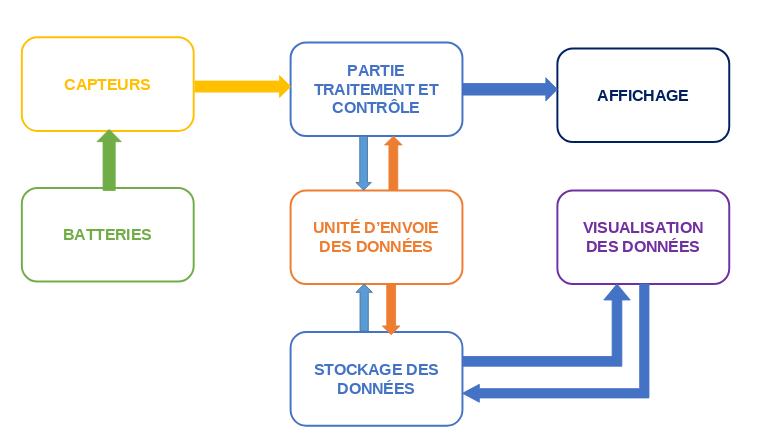
\includegraphics[width=17cm]{./img/schemaBloc.png}
	\caption{Schéma bloc du système général}
	\label{i1}
\end{figure}

Le système est composé de sept blocs distincts avec des fonctions précises. Nous allons détailler le fonctionnement de chaque bloc :

\paragraph{Bloc batterie :}
ce module est composé de trois batteries que le dispositif doit surveiller en temps réel.
\paragraph{Bloc des capteurs :}
cette section fournit les informations au reste du système. Elle est équipée des capteurs suivants :
\begin{itemize}
	\item Capteur de tension : mesure la tension de chaque batterie.
	\item Capteur de courant : mesure le courant de charge et de décharge de chaque batterie.
	\item Capteur de température :  évalue la température de chaque batterie. 
\end{itemize}

\paragraph{Unité de traitement et contrôle :}
cette partie constitue le cœur du dispositif. Elle analyse les données reçues des capteurs, effectue les calculs nécessaires, convertit les signaux analogiques en données exploitables par le système et héberge les programmes de contrôle.

\paragraph{Bloc d'affichage :}
cet élément est chargé de présenter les informations traitées par l'unité de contrôle de manière claire et accessible.

\paragraph{Unité d'envoi de données :}
il s’occupe de la communication des données traitées, selon les instructions de l'unité de traitement.

\paragraph{Centre de stockage :}
cette partie stocke les informations pré-traitées pour qu'elles puissent être utilisées pour surveiller l'état des batteries. Le stockage permet également de conserver un historique des données pour des analyses ultérieures.

\paragraph{Bloc de visualisation de données :}
ce bloc permet de visualiser les données en temps réel stockées par le centre de stockage.

\subsection{Principe de fonctionnement du dispositif}

Le but de ce dispositif est de surveiller en continu l'état de chaque batterie ainsi que celui de l'ensemble du système photovoltaïque.

La collecte des données sur les batteries se fait en deux étapes :

\begin{itemize} \item \textbf{Étape 1 :} mesure globale des batteries.
	À ce stade, nous collectons les données de tension, courant et température du système complet pour obtenir une vue d'ensemble du fonctionnement.
\item \textbf{Étape 2 :} mesure individuelle des batteries.  
Ici, chaque batterie est isolée pour effectuer des mesures précises de tension et de courant. Si cette opération se déroule pendant l'ensoleillement,il est possible de déconnecter le régulateur de charge afin d'éviter qu'il n'influence les valeurs mesurées par les capteurs. Nous procédons ainsi en séquence, en isolant chaque batterie l’une après l’autre, afin de déterminer leur état de fonctionnement et d'identifier celles qui nécessitent un remplacement.
\end{itemize}

\subsubsection{Organigramme}

Cet organigramme illustre la procédure logique à suivre pour assurer le bon fonctionnement de notre dispositif, en détaillant les étapes essentielles du processus de commande, de contrôle et d’exécution.



\begin{figure}[H]
	\centering
	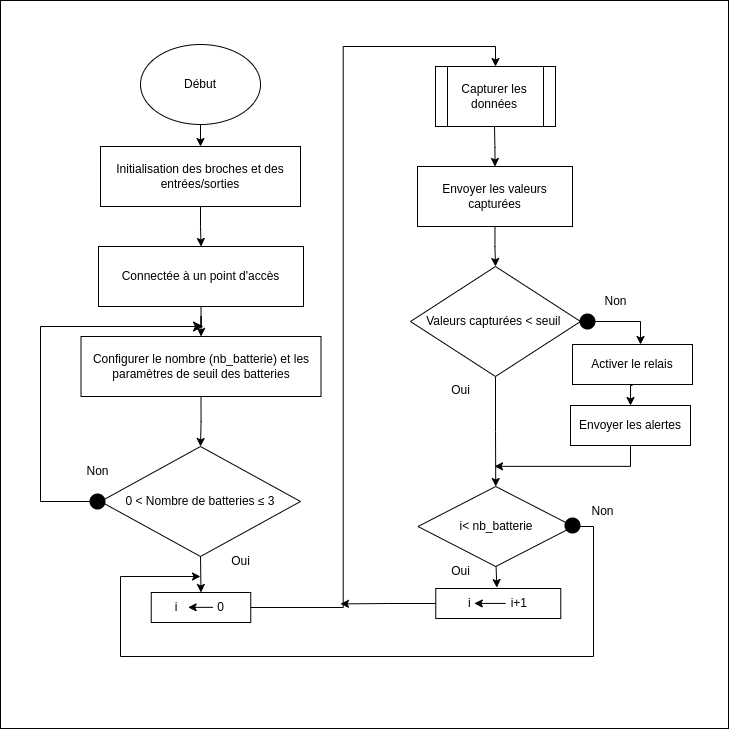
\includegraphics[width=15cm]{./img/organigramme.png}
	\caption{Organigramme du fonctionnement}
	\label{i1}
\end{figure}



\subsubsection{Étude d'une cas d'installation}

Pour nos étude on va prendre le cas d'une installation photovoltaïque qui à une puissance de 12Kw avec un tension de 400V.
On a vue dans le chapitre précèdent les procéder de dimensionnement d'une centrale photovoltaïque alors on va suivre ces étapes pour ce cas .


\subsubsection*{1. Besoin Énergétique des applications}
Supposons que les applications nécessitent une énergie totale de 12 kW en puissance crête.

\subsubsection*{2. Énergie solaire récupérable}
\begin{itemize}
	\item \textbf{Inclinaison et orientation des panneaux:}
	\begin{itemize}
		\item \textbf{Orientation:} les panneaux doivent être orientés vers le nord dans l'hémisphère sud pour maximiser la production.
		\item \textbf{Inclinaison:} pour Madagascar, une inclinaison égale à la latitude (environ 12°) est souvent recommandée \cite{pdf1}.
	\end{itemize}
	\item \textbf{Données météorologiques:} 
	supposons une irradiation moyenne de 5 kWh/m²/jour pour la période la moins ensoleillée.
\end{itemize}



%\begin{landscape}

\begin{table}[H]
	\centering
	\begin{tabular}{|>{\centering\arraybackslash}m{5cm}|>{\centering\arraybackslash}m{5cm}|>{\centering\arraybackslash}m{5cm}|}
		\hline
		\textbf{Calcul} & \textbf{Formule} & \textbf{Résultat} \\
		\hline
		\textbf{Énergie produite (Wh/jour)} & $E_p = \frac{E_c}{k}$ & $E_p = 17,143$ \text{ Wh/jour} \\
		\hline
		\textbf{Puissance crête } & $P_c = \frac{E_p}{Ir}$ & $P_c = 3,429$ \text{ W} \\
		\hline
		\textbf{Nombre de modules } & $N_p = \frac{P_c}{P_{pv}}$ & $N_p = 40$ \text{ modules} \\
		\hline
		\textbf{Nombre de panneaux en série } & $N_s = \frac{U}{V_m}$ & $N_s = 10$ \\
		\hline
		\textbf{Nombre de branches en parallèle } & $N_{bp} = \frac{N_p}{N_s}$ & $N_{bp} = 4$ \\
		\hline
		\textbf{Puissance crête d’un champ} & $P_{c/champ} = N_{bp} \times N_s \times P_{pv}$ & $P_{c/champ} = 12000$ \text{ W} \\
		\hline
		\textbf{Surface du générateur } & $S_t = S_m \times N_m$ & $S_t = 64$ \text{ m²} \\
		\hline
		\textbf{Capacité de batterie} & $C_j = \frac{E_c}{U}$ & $C_j = 30$ \text{ Ah/jour} \\
		\hline
		\textbf{Capacité totale des batteries} & $C_u = \frac{C_j \times N_j}{U \times P_d}$ & $C_u = 187,5$ \text{ Ah} \\
		\hline
		\textbf{Nombre de batteries} & $N_t = N_s \times N_p$ & $N_t = 18$ \text{ batteries} \\
		\hline
		\textbf{Courant maximal régulateur} & $I_{\text{max}} = \frac{P_{c/champ}}{U}$ & $I_{\text{max}} = 30$ \text{ A} \\
		\hline
		\textbf{Courant de sortie d’un panneau} & $I = \frac{P}{U}$ & $I = 7,5$ \text{ A} \\
		\hline
		\textbf{Section des câbles } & $S = \frac{\rho \cdot L}{R}$ & $S \approx 10$ \text{ mm²} \\
		\hline
		\textbf{Courant circulant entre batteries et onduleur} & $I_{\text{max batteries}} = \frac{P_{\text{max onduleur}}}{U_{\text{batterie}}}$ & $I_{\text{max batteries}} = 30$ \text{ A} \\
		\hline
	\end{tabular}
	\caption{Résumé des calculs pour le dimensionnement du système photovoltaïque}
	\label{tab:calculs_dimensionnement}
\end{table}
%\end{landscape}

\section{Les composantes électroniques adaptés au projet}

Selon le schéma bloc du système et les principes de fonctionnement décrits précédemment, plusieurs composants électroniques sont nécessaires pour réaliser le dispositif. Pour cette étude, nous prenons comme référence un dispositif capable de supporter une puissance maximale de 12 kW à la sortie de l'onduleur, avec une tension de 400 V et un courant de 30 A à l'entrée. Les composants requis pour cette configuration sont les suivants :

\subsection{Les capteurs et instruments de Mesure}

Des capteurs sont nécessaires pour surveiller le système et collecter des données pour le contrôle :

\subsubsection{Les capteurs de courant et de tension }
\subsubsection*{Pour le courant : modules ACS712 30A}

Le ACS712 utilise la technologie de l'effet Hall pour détecter le courant passant à travers le conducteur mesuré. L'effet Hall est un phénomène où une tension est générée perpendiculairement au flux de courant dans un matériau conducteur lorsqu'il est soumis à un champ magnétique  \cite{1}.

Il est conçu pour mesurer à la fois les courants AC et DC avec une grande précision, et sa sortie est un signal analogique qui varie en fonction de l'intensité du courant mesuré.


\begin{figure}[H]
	\centering
	\begin{subfigure}{0.40\textwidth} % Largeur de la première image
		\centering
		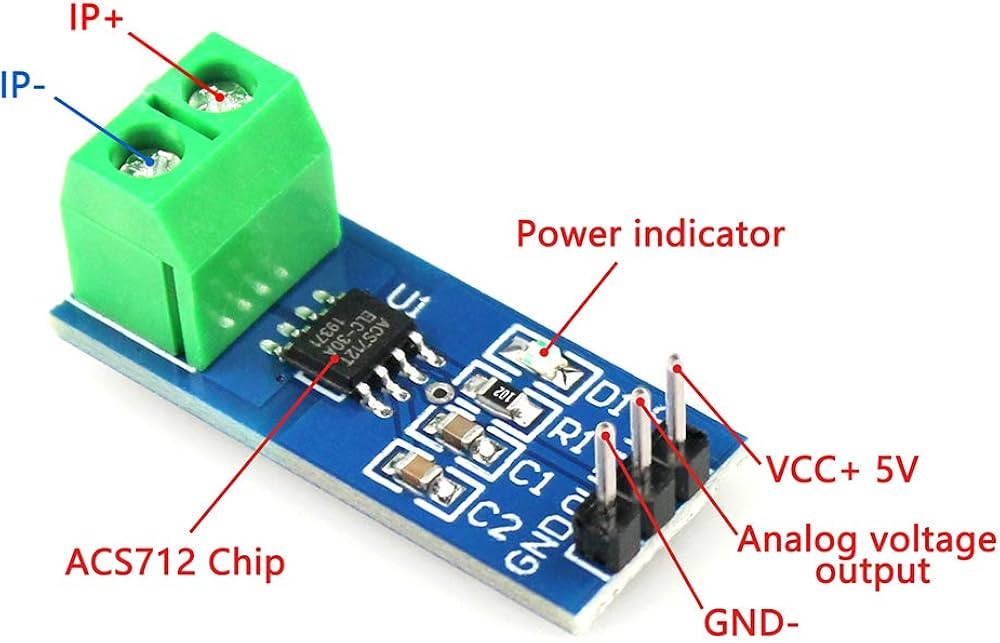
\includegraphics[width=\linewidth]{./img/composants/ACS712.jpg}
		\label{fig:acs712a}
	\end{subfigure}
	\hfill
	\begin{subfigure}{0.55\textwidth} % Largeur de la deuxième image
		\centering
		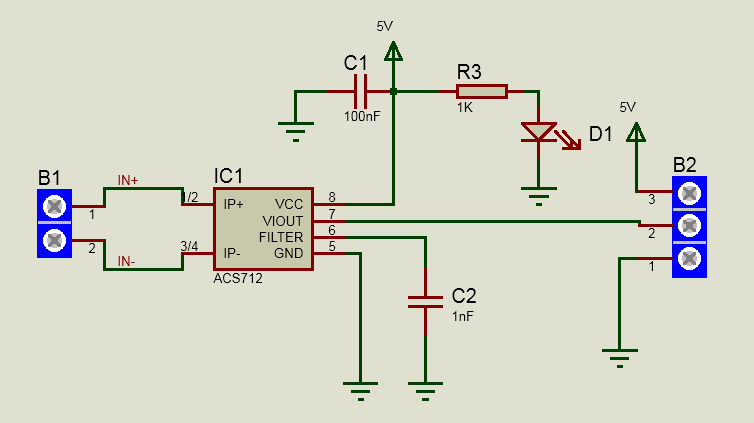
\includegraphics[width=\linewidth]{./img/composants/ACS.PNG}
		\label{fig:acs712b}
	\end{subfigure}
	\caption{Modules ACS712 30A  \cite{1} et son schéma}
	\label{fig:combined}
\end{figure}
\subsubsection*{Caractéristiques techniques }

\begin{itemize}
	\item \textbf{Plage de mesure du courant :} 
	\begin{itemize}
		\item De -30A à +30A (AC ou DC)
	\end{itemize}
	
	\item \textbf{Sensibilité (pour le modèle 30A) :}
	\begin{itemize}
		\item 66 mV par ampère (66 mV/A)
	\end{itemize}
	
	\item \textbf{Type de capteur :}
	\begin{itemize}
		\item Effet Hall (non-intrusif, sans contact direct avec le conducteur)
	\end{itemize}
	
	\item \textbf{Tension d'alimentation :} 
	\begin{itemize}
		\item 5V DC
	\end{itemize}
	
	\item \textbf{Tension de sortie :} 
	\begin{itemize}
		\item La tension de sortie du capteur est proportionnelle au courant mesuré. Lorsque le courant est nul, la sortie est à 2,5V (milieu de la plage d'alimentation). Les variations de courant font monter ou descendre cette tension :
		\begin{itemize}
			\item 0A $\rightarrow$ environ 2,5V
			\item Courant positif (jusqu’à 30A) $\rightarrow$ sortie augmente à partir de 2,5V
			\item Courant négatif (jusqu’à -30A) $\rightarrow$ sortie diminue à partir de 2,5V
		\end{itemize}
	\end{itemize}
	
	\item \textbf{Précision :}
	\begin{itemize}
		\item Erreur typique de ±1,5\%
	\end{itemize}
	
	\item \textbf{Tension d'isolation :}
	\begin{itemize}
		\item 2,1 kV RMS (entre la partie du circuit de puissance et la partie de mesure)
	\end{itemize}
	
	\item \textbf{Impédance interne (entrée) :}
	\begin{itemize}
		\item Très faible, donc une chute de tension négligeable à travers le capteur.
	\end{itemize}
	
	\item \textbf{Temps de réponse :}
	\begin{itemize}
		\item Typiquement 5 $\mu$s (rapide pour des mesures de courant dynamique)
	\end{itemize}
	
	\item \textbf{Largeur de bande :}
	\begin{itemize}
		\item 80 kHz
	\end{itemize}
	
	\item \textbf{Type de signal de sortie :}
	\begin{itemize}
		\item Analogique (à connecter à une entrée analogique d'un microcontrôleur ou d'une carte d'acquisition de données)
	\end{itemize}
\end{itemize}


\subsubsection*{Pour la tension : diviseur de tension}

Un diviseur de tension est un circuit simple constitué de deux résistances connectées en série, utilisé pour réduire la tension d'entrée à une valeur proportionnelle à la tension souhaitée. Ce type de circuit est souvent utilisé pour mesurer des tensions élevées, comme celles des batteries solaires, et les adapter à la plage de mesure des capteurs ou des microcontrôleurs.

\begin{figure}[H]
	\centering
	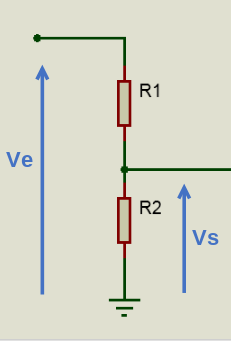
\includegraphics[width=3cm]{./img/composants/DDT.png}
	\caption{Schéma d'un diviseur de tension }
	\label{i1}
\end{figure}



\subsubsection*{Caractéristiques techniques}

\textbf{Tension d'entrée (Ve)} :
\begin{itemize}
	\item La tension de la batterie solaire (par exemple, 12V, 24V ou 48V) est appliquée au point d'entrée du diviseur de tension.
	\item La tension d'entrée maximale dépend des résistances sélectionnées et de la capacité des composants à dissiper la puissance.
\end{itemize}

\textbf{Tension de sortie (Vs)} :
\begin{itemize}
	\item La tension de sortie est proportionnelle à la tension d'entrée selon la formule :
	\begin{equation}
		V_{s} = V_{e} \times \frac{R2}{R1 + R2}
	\end{equation}
	\item Cette sortie est souvent adaptée à une tension de 5V ou 3.3V pour être compatible avec les entrées analogiques des microcontrôleurs comme l'Arduino ou l'ESP32.
\end{itemize}

\textbf{Précision} :
\begin{itemize}
	\item La précision dépend de la tolérance des résistances. Utiliser des résistances avec une faible tolérance (1\% ou moins) améliore la précision du diviseur.
\end{itemize}

\textbf{Puissance dissipée} :
\begin{itemize}
	\item Les résistances doivent être choisies en fonction de leur capacité à dissiper la chaleur. La puissance dissipée par chaque résistance est calculée comme :

	
	\begin{equation}
		P = \frac{V^2}{R}
	\end{equation}
\end{itemize}

\subsubsection{Capteurs de température LM35}
Le LM35 est un capteur de température de précision dont la sortie est proportionnelle à la température ambiante mesurée. Le LM35 produit une sortie en tension linéaire avec la température en degrés Celsius, ce qui le rend facile à utiliser avec les microcontrôleurs et les systèmes de mesure analogiques sans avoir besoin de conversion de température  \cite{3}.

\begin{figure}[H]
	\centering
	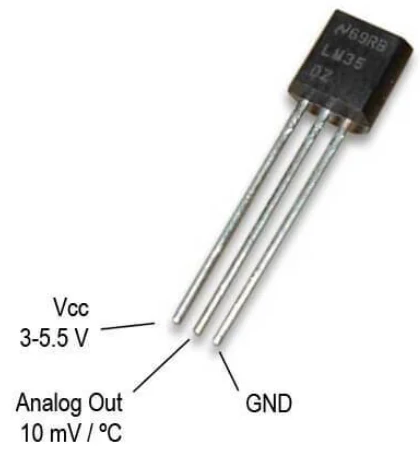
\includegraphics[width=4cm]{./img/composants/LM35.png}
	\caption{Le capteur LM35}
	\label{i1}
\end{figure}

\subsubsection*{Caractéristiques Techniques du LM35}
\begin{itemize}
	\item \textbf{Plage de température mesurable} : -55°C à +150°C
	\item \textbf{Précision} : 
	\begin{itemize}
		\item ±0.5°C à 25°C
		\item ±0.75°C sur la plage complète
	\end{itemize}
	\item \textbf{Tension de sortie} : 10 mV/°C
	\item \textbf{Tension d'alimentation} : 4V à 30V
	\item \textbf{Courant d'alimentation} : Typiquement 60 µA
	\item \textbf{Impédance de sortie} : $\ 0.1 \Omega $ (pour un courant de sortie jusqu’à 1 mA)
	\item \textbf{Temps de réponse} : 1 seconde (pour 63\% de variation)
	\item \textbf{Linéarité} : Sortie linéaire par rapport à la température
	\item \textbf{Compatibilité} : Compatible avec les entrées analogiques des microcontrôleurs
\end{itemize}

\subsection{Partie traitement et contrôle}
\subsubsection{Microcontrôleur ESP 32 WROOM 32}
\textbf{Déscription}

Suite au succès de l'ESP8266, l'ESP32 a été introduit, offrant des performances nettement supérieures à son prédécesseur. L'ESP32 est une série de microcontrôleurs SoC (System on Chip) développée par Espressif Systems, reposant sur l'architecture Xtensa LX6 de Tensilica, avec des fonctionnalités intégrées pour le Wi-Fi et le Bluetooth. Parmi les outils de développement disponibles, on retrouve l'Arduino IDE, un logiciel libre conçu en C++, qui inclut un grand nombre de bibliothèques, ainsi que de nombreuses bibliothèques tierces dédiées aux applications embarquées et temps réel  \cite{5}.\\

\textbf{La structure externe et structure interne }\\
Voici les structures externe et interne du microcontrôleur ESP32 présentées ci-dessous :
\begin{figure}[H]
	\centering
	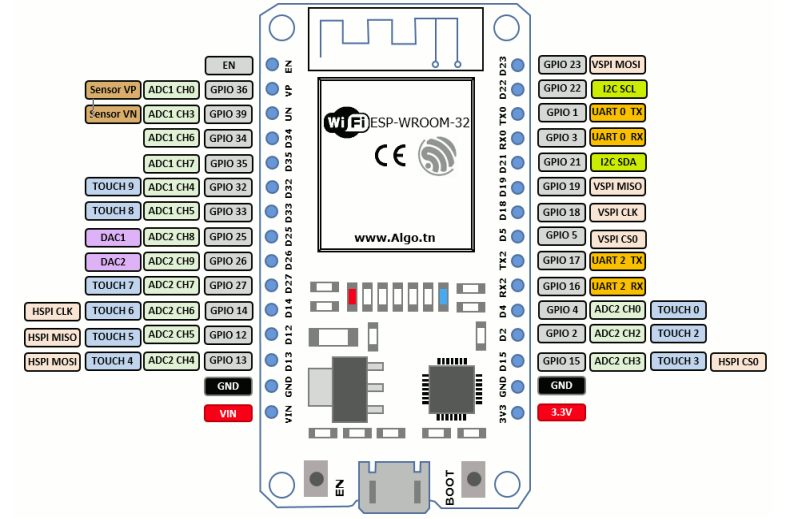
\includegraphics[width=15cm]{./img/composants/esp.png}
	\caption{La structure externe  \cite{8} }
	\label{i1}
\end{figure}



\begin{figure}[H]
	\centering
	\begin{subfigure}{0.40\textwidth} % Largeur de la première image
		\centering
		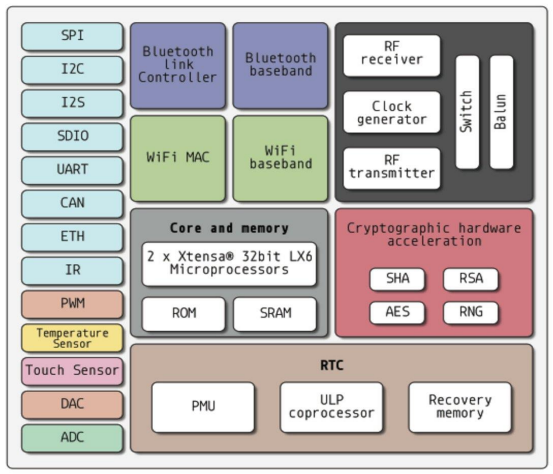
\includegraphics[width=9cm]{./img/composants/espInterne.png}
		\caption{La structure interne \cite{8} }
		\label{i1}
	\end{subfigure}
	\hfill
	\begin{subfigure}{0.55\textwidth} % Largeur de la deuxième image
			\centering
		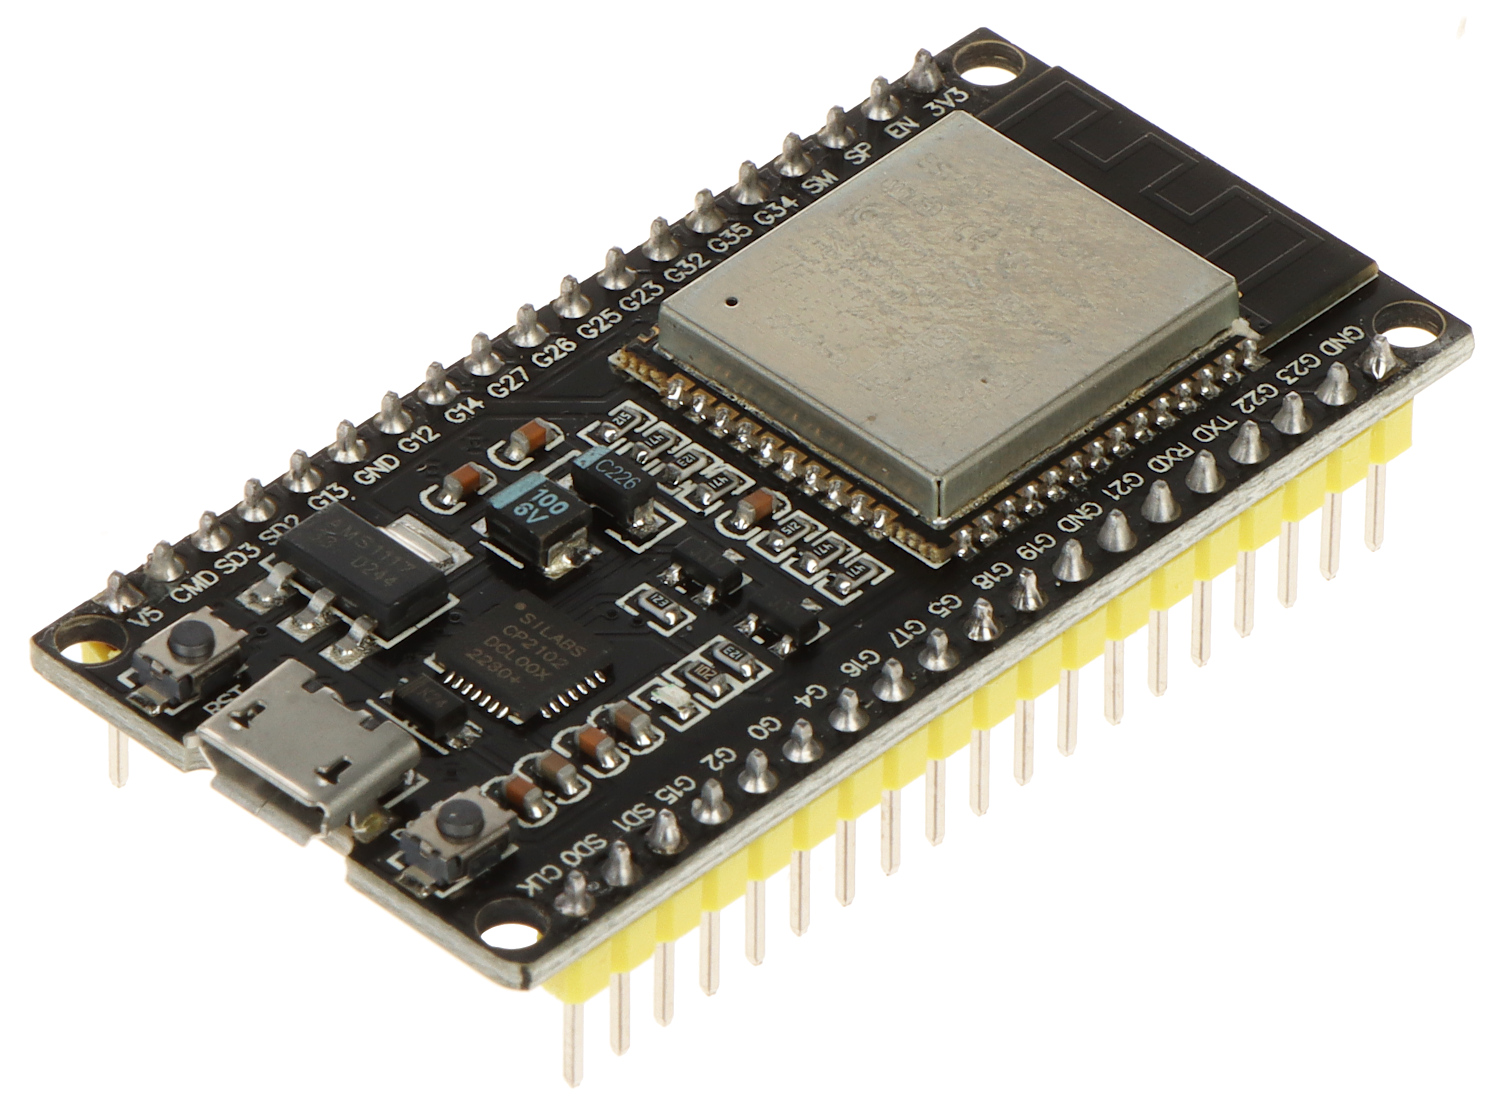
\includegraphics[width=5cm]{./img/composants/ESP.jpg}
		\caption{L'ESP 32 WROOM 32  \cite{5} }
		\label{i1}
	\end{subfigure}
\end{figure}

\subsubsection*{Ses principales spécifications techniques sont les suivantes :}

\begin{itemize}
	\item \textbf{Processeur :} microprocesseur Xtensa double cœur 32 bits, fonctionnant à 160 ou 240 MHz, offrant jusqu'à 600 MIPS.
	\item \textbf{Mémoire :}
	\begin{itemize}
		\item ROM : 448 Ko
		\item Flash : 4 Mo
		\item RAM : 520 Ko de SRAM
	\end{itemize}
	\item \textbf{Ressources :}
	\begin{itemize}
		\item Broches : 32 GPIO avec ADC (12), DAC (2), SPI (3), I2S (2), I2C (2), UART (3), PWM (32), SDIO (50 MHz)
		\item Connectivité sans fil :
		\begin{itemize}
			\item Wi-Fi : 802.11 b/g/n à 2,4 GHz, avec un débit maximal de 150 Mbps
			\item Bluetooth
		\end{itemize}
		\item Contrôleur infrarouge intégré
		\item Capteur à effet Hall
		\item Préamplificateur analogique intégré
	\end{itemize}
	\item \textbf{Consommation énergétique :} Très faible
	\item \textbf{Plage de température de fonctionnement :} -40°C à 125°C
	\item \textbf{Tension d'alimentation :} 2,2V à 3,6V DC
\end{itemize}


Le ESP32 est choisi pour sa capacité à gérer les communications sans fil et son support pour de multiples interfaces de capteurs et actuateurs, ce qui le rend idéal pour les applications IoT dans un système photovoltaïque.

\subsection{Afficheur LCD avec module I2C}
Le module LCD 2x16 est un écran à cristaux liquides qui peut afficher deux lignes de 16 caractères chacune. Lorsqu'il est combiné avec un module I2C, il permet de contrôler l'écran avec seulement deux fils pour la communication (SDA et SCL) en plus de l'alimentation. Cela simplifie grandement les connexions et le câblage, rendant le LCD plus facile à utiliser avec des microcontrôleurs  \cite{6}.
\begin{figure}[H]
	\centering
	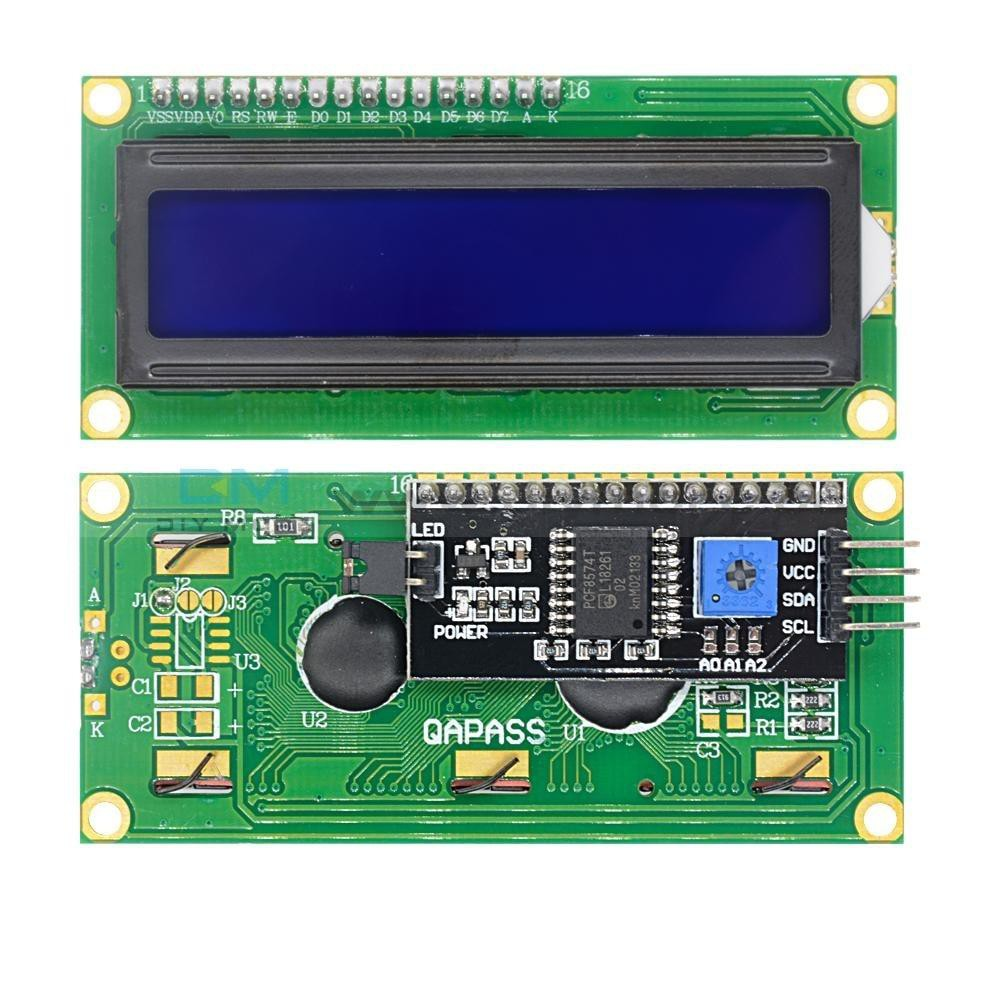
\includegraphics[width=6cm]{./img/composants/lcdI2C.jpeg}
	\caption{Le LCD 2x16 avec module I2C  \cite{6}}
	\label{i1}
\end{figure}
\subsubsection*{Caractéristiques du LCD 2x16 avec I2C}

\begin{itemize}[label={--}]
	\item \textbf{Dimensions de l'écran} : 2 lignes x 16 caractères.
	\item \textbf{Type de module} : LCD 16x2 avec interface I2C.
	\item \textbf{Affichage} : LCD à rétroéclairage LED
	\item \textbf{Interface I2C} : Communication via SDA (données) et SCL (horloge).
	\item \textbf{Alimentation} : 5V
	\item \textbf{Adresse I2C} : Souvent 0x27 ou 0x3F.
	\item \textbf{Commandes et fonctionnalités} : commandes LCD standards, affichage de texte et caractères spéciaux.
	\item \textbf{Consommation d'énergie} : faible, adapté aux projets alimentés par batterie.
	\item \textbf{Connectivité} : 4 broches (VCC, GND, SDA, SCL).
\end{itemize}

\subsection{Module de Communication}

Le module de communication permet d’envoyer les données collectées vers une plateforme en ligne, facilitant le suivi à distance. Le module GSM SIM900 est utilisé pour sa compatibilité avec les réseaux GSM/GPRS.\\

\textbf{Module GSM SIM900 :} Utilisé dans les applications IoT pour la communication sans fil, ce module permet la transmission de données par SMS ou GPRS.

\begin{itemize} \item \textbf{Caractéristiques techniques :}
	
	\begin{itemize}
		\item \textbf{Fréquences GSM :} quadri-bande (850, 900, 1800, 1900 MHz), compatible avec la plupart des réseaux mondiaux.
		
		\item \textbf{Interface UART :} communication avec microcontrôleurs via UART, configurable jusqu'à 115200 bps. Commandes AT pour gérer les SMS et la transmission de données (`AT+CMGF`, `AT+CMGS`).
		
		\item \textbf{GPRS classe 10 :} débit maximal de 85.6 kbps pour la transmission de données TCP/IP. Compatible avec les protocoles HTTP et FTP pour l'envoi de données à un serveur distant.
		
		\item \textbf{Alimentation :} fonctionne entre 3.2V et 4.8V, avec une consommation de 1.5 mA en veille et jusqu’à 2A lors des pics de transmission.
		
		\item \textbf{Mode d’économie d’énergie :} mode veille (1.5 mA) pour prolonger l’autonomie dans les applications à basse consommation.
	\end{itemize}
	
	\begin{figure}[H]
		\centering
		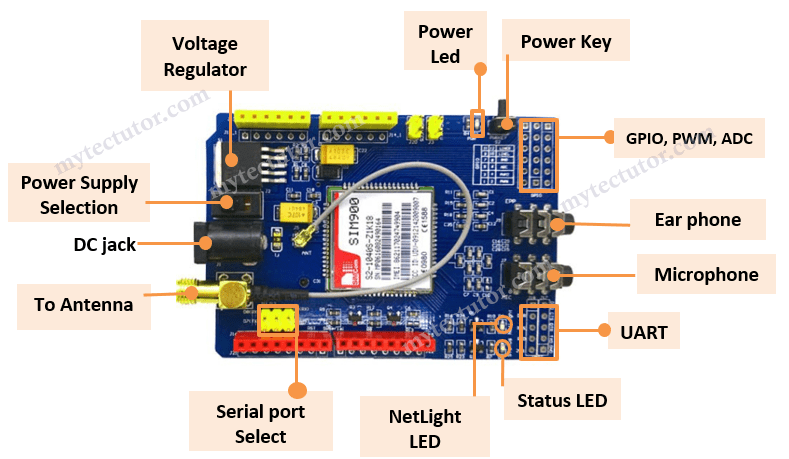
\includegraphics[width=12cm]{./img/composants/SIM900.png}
		\caption{Le module GSM SIM900 \cite{7}}
		\label{i1}
	\end{figure}
	
	\item \textbf{Avantages :}
	\begin{itemize}
		\item \textbf{Fiabilité :} adapté aux environnements éloignés grâce à la couverture GSM étendue.
		\item \textbf{Faible coût :} rentable pour les projets IoT nécessitant une connectivité cellulaire.
		\item \textbf{Compatibilité :} facile à intégrer avec des microcontrôleurs via UART et commandes AT.
	\end{itemize}
	
	\item \textbf{Inconvénients :}
	\begin{itemize}
		\item \textbf{Débit limité :} GPRS offre un débit faible comparé aux technologies modernes (3G/4G).
		\item \textbf{Consommation d’énergie élevée :} pics de consommation jusqu’à 2A lors des transmissions GPRS.
	\end{itemize}
	
 \end{itemize}


\subsection{Module relais 5V DC}
\subsubsection*{Description}
Le module relais 5V DC permet de contrôler des charges à haute tension à l'aide de signaux de faible puissance provenant de microcontrôleurs ou autres circuits de commande. Grâce à son système d'isolation, il protège le circuit de commande contre les surtensions et interférences provenant du côté de la charge \cite{2}.

\subsubsection*{Caractéristiques}

\begin{itemize}[label={--}]
	\item \textbf{Type de relais} : Relais électromagnétique.
	\item \textbf{Tension de commande} : 5V DC.
	\item \textbf{Capacité de charge} : 
	\begin{itemize}[label={*}]
		\item \textbf{AC} : Jusqu'à 250V AC, 10A.
		\item \textbf{DC} : Jusqu'à 30V DC, 10A.
	\end{itemize}
	\item \textbf{Connectivité} :
	\begin{itemize}[label={*}]
		\item \textbf{Broches de contrôle} : IN1, IN2, etc. pour les signaux de commande.
		\item \textbf{Broches d'alimentation} : VCC, GND pour l'alimentation du module.
		\item \textbf{Broches de relais} : COM, NO (Normalement Ouvert), NC (Normalement Fermé) pour la connexion de la charge.
	\end{itemize}
	\item \textbf{Indicateur LED} : LEDs pour indiquer l'état de chaque relais.
	\item \textbf{Isolation} : isolation optique entre le circuit de commande et le circuit de charge, réalisée à l'aide d'un optocoupleur.
\end{itemize}

\subsubsection*{Isolation}
L'isolation protège le microcontrôleur contre les surtensions et interférences provenant du circuit de puissance. Le module relais utilise un \textbf{optocoupleur} (\textbf{PC817}) pour assurer une isolation galvanique, permettant de transmettre un signal sans connexion physique directe. Cela aide à :
\begin{itemize}[label={*}]
	\item \textbf{Protéger le microcontrôleur} des hautes tensions.
	\item \textbf{Réduire les interférences électromagnétiques.}
	\item \textbf{Assurer la sécurité électrique.}
\end{itemize}

\textbf{Fonctionnement de l'optocoupleur} : 
nn optocoupleur est un composant qui utilise une diode LED pour transmettre des signaux électriques à travers la lumière. Le côté commande active la LED interne de l'optocoupleur, qui est détectée par un phototransistor du côté relais. Ainsi, le microcontrôleur reste isolé de la partie haute tension du circuit.

%\begin{figure}[H]
%	\centering
%	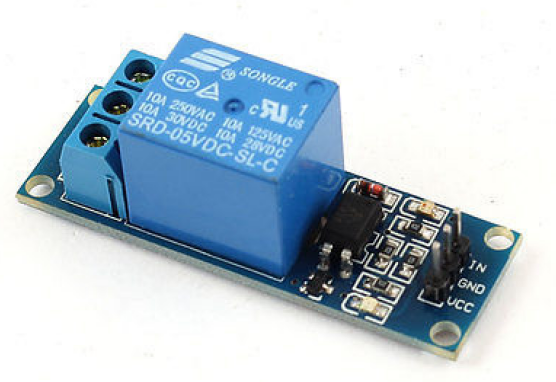
\includegraphics[width=6cm]{./img/composants/relais.png}
%	\caption{Module relais 5V DC}
%	\label{fig:relais_5vdc}
%\end{figure}
	
	
	
	\begin{figure}[H]
		\centering
		\begin{subfigure}{0.25\textwidth} % Largeur de la première image
			\centering
			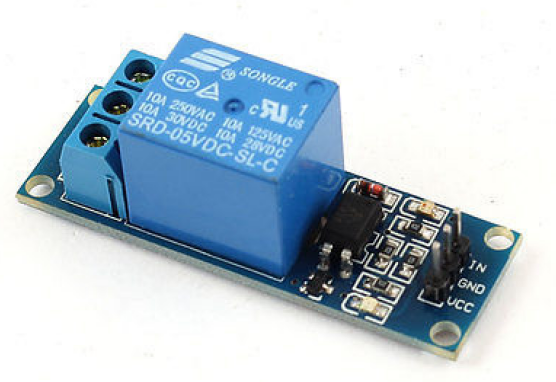
\includegraphics[width=\linewidth]{./img/composants/relais.png}
			\label{fig:acs712a}
		\end{subfigure}
		\hfill
		\begin{subfigure}{0.70\textwidth} % Largeur de la deuxième image
			\centering
			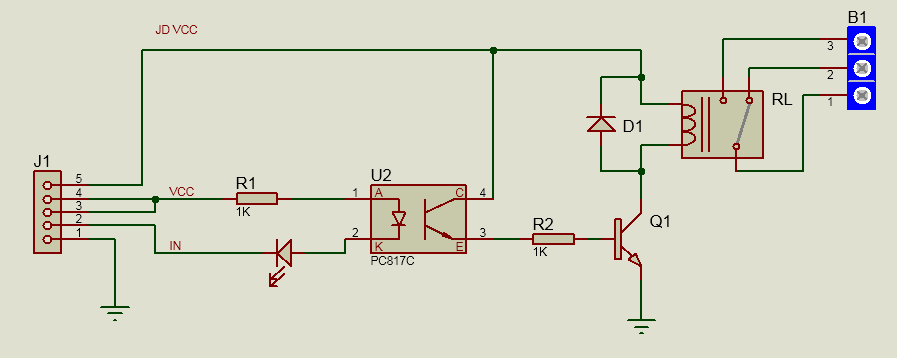
\includegraphics[width=12cm]{./img/composants/relais.PNG}
			\label{fig:acs712b}
		\end{subfigure}
		\caption{Module relais 5V DC \cite{2} et son schéma}
		\label{fig:combined}
	\end{figure}
	
\subsection{Transistor 2N2222}
	
	Pour éviter de surcharger le microcontrôleur, nous allons utiliser un transistor bipolaire en mode commutation. Un transistor nécessite seulement un faible courant pour atteindre l'état de saturation. Le modèle que nous choisirons est le 2N2222, un transistor bipolaire. Ses caractéristiques sont les suivantes \cite{9}:
	
\begin{itemize}[label={--}]
	\item \textbf{Type} : NPN
	\item \textbf{Tension maximale collecteur-émetteur} : 30 V
	\item \textbf{Courant continu collecteur} : 800 mA
	\item \textbf{Dissipation de puissance} : 500 mW
	\item \textbf{Fréquence de transition} : 250 MHz
	\item \textbf{Gain en courant DC (hFE min)} : 100
	\item \textbf{Plage de température de fonctionnement} : -65°C à +200°C
\end{itemize}
\begin{figure}[H]
	\centering
	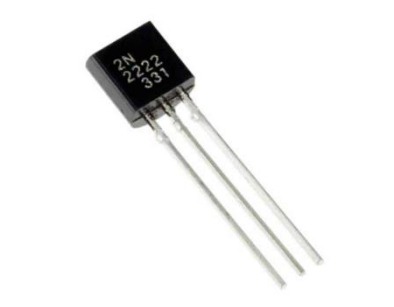
\includegraphics[width=6cm]{./img/composants/2n2222.png}
	\caption{Le transistor 2N2222}
	\label{fig:relais_5vdc}
\end{figure}
\subsection{Diode Zener 1N4728A}

\subsubsection*{Description}
La diode Zener 1N4728A est une diode à effet Zener conçue pour la régulation de tension et la protection contre les surtensions. Elle maintient une tension constante de 3.3V lorsqu'une tension plus élevée est appliquée dans la direction inverse, protégeant ainsi des composants sensibles comme l'ESP32 \cite{4}.

\subsubsection*{Caractéristiques}

\begin{itemize}[label={--}]
	\item \textbf{Type} : Diode Zener
	\item \textbf{Tension Zener} : 3.3 V (tension de régulation)
	\item \textbf{Courant Zener nominal} : 76mA
	\item \textbf{Puissance dissipée maximale} : 500 mW
	\item \textbf{Température de fonctionnement} : -65°C à +150°C
	\item \textbf{Tension inverse maximale} : 100 V
	\item \textbf{Tolérance de la tension Zener} : ±5\%
\end{itemize}
\begin{figure}[H]
	\centering
	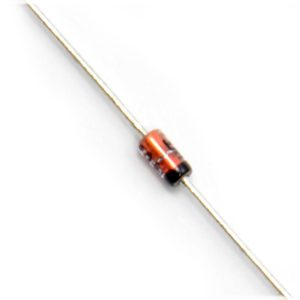
\includegraphics[width=4cm]{./img/composants/1n4728.jpg}
	\caption{Le diode zener 1N4728A}
	\label{fig:relais_5vdc}
\end{figure}
\section{Le système multi-capteurs contrôlé par ESP32}

Le dispositif de monitoring des batteries solaires est conçu pour capturer les paramètres clés des batteries et du système, tels que les tensions, les courants et les températures de chaque batterie. Pour mesurer les courants et les températures des batteries, le système utilise des capteurs ACS712 et LM35 respectivement. La tension des batteries est mesurée à l'aide d'un diviseur de tension qui réduit la tension à un niveau compatible avec les entrées analogiques de l'ESP32.

Pour garantir une mesure précise et efficace, chaque batterie est isolée par des relais. Les trois relais sont alternés pour activer et désactiver chaque batterie successivement. Un relais supplémentaire est connecté au régulateur de charge afin de l'isoler et obtenir des mesures fiables, que ce soit durant l'ensoleillement ou la nuit.

Les données capturées par les capteurs sont traitées par le microcontrôleur ESP32, qui est responsable de l'analyse, du traitement et de la commande des relais. Les informations traitées par l'ESP32 sont affichées sur un écran LCD et transmises à une base de données en ligne pour le stockage. L'ESP32 recueille également les paramètres configurés par l'utilisateur.

La transmission des données se fait principalement par Wi-Fi, grâce au module intégré de l'ESP32.

\begin{figure}[H]
	\centering
	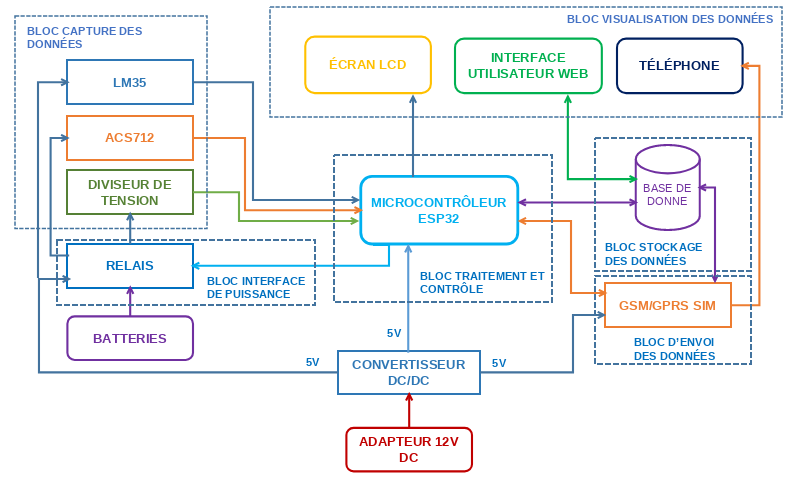
\includegraphics[width=17cm]{./img/composants/SCHEMAFONCTIONNEL.png}
	\caption{Le schéma fonctionnel}
	\label{fig:relais_5vdc}
\end{figure}


%\section{Étalonnage des capteurs}

%Afin d'assurer un fonctionnement optimal de nos capteurs de température, de courant et de tension, il est nécessaire de passer par des étapes d’étalonnage. Ce processus consiste à ajuster les capteurs afin de corriger les écarts de mesure et d'assurer des résultats précis.

%Dans notre projet, nous disposons de plusieurs capteurs : 4 capteurs ACS712 pour mesurer le courant, 4 diviseurs de tension pour mesurer la tension, et 3 capteurs LM35 pour mesurer la température. Pour garantir la précision des mesures, chaque capteur sera étalonné individuellement.

%\subsubsection{Étalonnage des capteurs ACS712}

%\textbf{Capteur ACS712 numéro 01 :}

%\begin{table}[H]
%	\centering
%	\begin{tabular}{|>{\centering\arraybackslash}m{4cm}|>{\centering\arraybackslash}m{3cm}|>{\centering\arraybackslash}m{3cm}|>{\centering\arraybackslash}m{3cm}|}
%		\hline
%		\textbf{Valeurs de l’étalon de référence (A)} & \textbf{Valeurs du capteur (A)} & \textbf{Écart de mesure (A)} & \textbf{Écart de mesure (\%)} \\
%		\hline
%		0.5 & 0.48 & -0.02 & -4.0 \\
%		1.0 & 0.98 & -0.02 & -2.0 \\
%		1.5 & 1.46 & -0.04 & -2.7 \\
%		2.0 & 1.98 & -0.02 & -1.0 \\
%		\hline
%	\end{tabular}
%	\caption{Étalonnage du capteur ACS712 numéro 01}
%	\label{tab:acs712_01}
%\end{table}

%\textbf{Capteur ACS712 numéro 02 :}

%\begin{table}[H]
%	\centering
%	\begin{tabular}{|>{\centering\arraybackslash}m{4cm}|>{\centering\arraybackslash}m{3cm}|>{\centering\arraybackslash}m{3cm}|>{\centering\arraybackslash}m{3cm}|}
%		\hline
%		\textbf{Valeurs de l’étalon de référence (A)} & \textbf{Valeurs du capteur (A)} & \textbf{Écart de mesure (A)} & \textbf{Écart de mesure (\%)} \\
%		\hline
%		0.5 & 0.49 & -0.01 & -2.0 \\
%		1.0 & 0.97 & -0.03 & -3.0 \\
%		1.5 & 1.47 & -0.03 & -2.0 \\
%		2.0 & 2.01 & +0.01 & +0.5 \\
%		\hline
%	\end{tabular}
%	\caption{Étalonnage du capteur ACS712 numéro 02}
%	\label{tab:acs712_02}
%\end{table}

%\textbf{Capteur ACS712 numéro 03 :}

%\begin{table}[H]
%%	\begin{tabular}{|>{\centering\arraybackslash}m{4cm}|>{\centering\arraybackslash}m{3cm}|>{\centering\arraybackslash}m{3cm}|>{\centering\arraybackslash}m{3cm}|}
%		\hline
%		\textbf{Valeurs de l’étalon de référence (A)} & \textbf{Valeurs du capteur (A)} & \textbf{Écart de mesure (A)} & \textbf{Écart de mesure (\%)} \\
%		\hline
%		0.5 & 0.47 & -0.03 & -6.0 \\
%		1.0 & 0.99 & -0.01 & -1.0 \\
%		1.5 & 1.45 & -0.05 & -3.3 \\
%		2.0 & 2.02 & +0.02 & +1.0 \\
%		\hline
%	\end{tabular}
%	\caption{Étalonnage du capteur ACS712 numéro 03}
%	\label{tab:acs712_03}
%\end{table}

%\textbf{Capteur ACS712 numéro 04 :}

%\begin{table}[H]
%	\centering
%	\begin{tabular}{|>{\centering\arraybackslash}m{4cm}|>{\centering\arraybackslash}m{3cm}|>{\centering\arraybackslash}m{3cm}|>{\centering\arraybackslash}m{3cm}|}
%		\hline
%		\textbf{Valeurs de l’étalon de référence (A)} & \textbf{Valeurs du capteur (A)} & \textbf{Écart de mesure (A)} & \textbf{Écart de mesure (\%)} \\
%		\hline
%		0.5 & 0.49 & -0.01 & -2.0 \\
%%		1.5 & 1.47 & -0.03 & -2.0 \\
%%%	\end{tabular}
%	\caption{Étalonnage du capteur ACS712 numéro 04}
%%end{table}

%\subsubsection{Étalonnage des capteurs LM35}

%\textbf{Capteur LM35 numéro 01 :}

%\begin{table}[H]
%	\centering
%\begin{tabular}{|>{\centering\arraybackslash}m{4cm}|>{\centering\arraybackslash}m{3cm}|>{\centering\arraybackslash}m{3cm}|>{\centering\arraybackslash}m{3cm}|}
%		\hline
%		\textbf{Valeurs de l’étalon de référence (°C)} & \textbf{Valeurs du capteur (°C)} & \textbf{Écart de mesure (°C)} & \textbf{Écart de mesure (\%)} \\
%		\hline
%		0 & -0.1 & -0.1 & -10.0 \\
%		25 & 24.8 & -0.2 & -0.8 \\
%%		75 & 74.9 & -0.1 & -0.1 \\
%		\hline
%	\end{tabular}
%	\caption{Étalonnage du capteur LM35 numéro 01}
%	\label{tab:lm35_01}
%\end{table}

%\textbf{Capteur LM35 numéro 02 :}

%\begin{table}[H]
%%	\begin{tabular}{|>{\centering\arraybackslash}m{4cm}|>{\centering\arraybackslash}m{3cm}|>{\centering\arraybackslash}m{3cm}|>{\centering\arraybackslash}m{3cm}|}
%%		\textbf{Valeurs de l’étalon de référence (°C)} & \textbf{Valeurs du capteur (°C)} & \textbf{Écart de mesure (°C)} & \textbf{Écart de mesure (\%)} \\
%		\hline
%%		25 & 24.6 & -0.4 & -1.6 \\
%		50 & 50.2 & +0.2 & +0.4 \\
%		75 & 74.7 & -0.3 & -0.4 \\
%		\hline
%	\end{tabular}
%	\caption{Étalonnage du capteur LM35 numéro 02}
%	\label{tab:lm35_02}
%\end{table}

%\subsubsection{Étalonnage des diviseurs de tension}

%\textbf{Diviseur de tension numéro 01 :}

%\begin{table}[H]
%	\centering
%	\begin{tabular}{|>{\centering\arraybackslash}m{4cm}|>{\centering\arraybackslash}m{3cm}|>{\centering\arraybackslash}m{3cm}|>{\centering\arraybackslash}m{3cm}|}
%		\hline
%		\textbf{Valeurs de l’étalon de référence (V)} & \textbf{Valeurs du capteur (V)} & \textbf{Écart de mesure (V)} & \textbf{Écart de mesure (\%)} \\
%		\hline
%		5.0 & 5.05 & +0.05 & +1.0 \\
%		10.0 & 9.95 & -0.05 & -0.5 \\
%		15.0 & 15.05 & +0.05 & +0.3 \\
%		20.0 & 19.95 & -0.05 & -0.3 \\
%		\hline
%	\end{tabular}
%	\caption{Étalonnage du diviseur de tension numéro 01}
%	\label{tab:diviseur_01}
%\end{table}


%Chaque capteur a été étalonné individuellement, et les écarts de mesure ont été évalués pour chaque cas. Les résultats indiquent de petites différences entre les valeurs mesurées par les capteurs et les valeurs de référence, avec des écarts en pourcentage généralement faibles. Ces observations confirment que l'étalonnage a efficacement corrigé les erreurs de mesure initiales.

%Le tableau suivant présente les valeurs de l’étalon de référence ainsi que les valeurs mesurées par les capteurs après l’étalonnage, avec les corrections appliquées.% Les mesures ont été réalisées à intervalles réguliers de 15 minutes, ce qui permet d'observer l'évolution des écarts au fil du temps et d'évaluer la précision des capteurs dans des conditions réelles d'utilisation.

%\subsubsection{Test paramétrique}
%Afin de vérifier si la distribution des données suit une loi normale (distribution gaussienne), nous appliquons un test de normalité. Pour cela, nous utilisons des indicateurs statistiques tels que l'asymétrie et l'aplatissement. Un échantillon est considéré comme suivant une loi normale à un niveau de confiance de 95 \% lorsque les valeurs de l'asymétrie et de l'aplatissement se situent dans l'intervalle de -2 à +2.

%\textbf{Asymétrie} : \\
%L'asymétrie mesure la symétrie de la distribution des données. Elle est calculée par la formule suivante :


%\begin{equation}
%G_T1 = \frac{n}{(n - 1)(n - 2)} \sum_{i=1}^{n} \left( \frac{x_i - \overline{x}}{S_T} \right)^3
%\end{equation}

%D'après nos calculs (voir annexe), nous obtenons une valeur d’asymétrie de :
%\[
%G_T1 = -0,27
%\]

%\textbf{Aplatissement} : \\
%L’aplatissement indique la "plateur" de la distribution. Il est obtenu à partir de la formule suivante :
%\begin{equation}
%G_{T2} = \frac{n(n + 1)}{(n - 1)(n - 2)(n - 3)} \sum_{i=1}^{n} \left( \frac{x_i - \overline{x}}{S_T} \right)^4 - \frac{3(n - 1)^2}{(n - 2)(n - 3)}
%\end{equation}

%Après calcul (voir annexe), nous trouvons la valeur suivante pour l'aplatissement :
%\[
%G_T2 = -0,78
%\]

%Les échantillons de mesures de tension, de courant et de température, après correction et étalonnage, suivent une loi normale à 95 \% car les valeurs de leurs aplatissements et de leurs asymétries se situent toutes dans l'intervalle compris entre -2 et 2.

\section{Conclusion}

Dans ce chapitre, nous avons exposé le principe de fonctionnement du dispositif en détaillant à la fois le schéma bloc et le schéma fonctionnel. Nous avons également effectué une étude approfondie des composants électroniques utilisés, justifiant ainsi le choix des composants retenus pour ce projet. Chaque élément a été sélectionné en fonction de ses caractéristiques techniques et de son adéquation avec les exigences du système de monitoring des batteries solaires.

Dans le chapitre suivant, nous aborderons en détail la partie relative à l’envoi des données, ainsi que la structure de la base de données destinée à stocker les informations collectées. Nous y explorerons les méthodes de transmission et de gestion des données pour assurer un suivi en temps réel.

	%\chapter{Fonctionnement générale du système }
\phantomsection
\addcontentsline{toc}{chapter}{Fonctionnement générale du système} 

\section{Introduction}

Dans ce chapitre, nous allons présenter en détail la conception et la réalisation de notre système de suivi en temps réel des batteries solaires. Nous expliquons les choix technologiques et les méthodes employées pour mesurer et surveiller les paramètres critiques abordés dans le chapitre précédent.

\subsection{Présentation générale du dispositif} Le dispositif est conçu pour surveiller en temps réel les paramètres essentiels de trois batteries solaires utilisées dans une installation photovoltaïque. Ce système capture des données telles que la tension, le courant et la température de chaque batterie individuellement, que les batteries soient montées en série ou en parallèle. Il fournit également des informations sur l'état de charge (SoC) et l'état de décharge (DoD) du système. En cas d'anomalie, le dispositif peut envoyer une alerte par SMS ou par email via l'application web, grâce à l'utilisation d'un microcontrôleur.

\subsection{Analyse des besoins du dispositif} 
Avant de concevoir le dispositif, il est essentiel de comprendre ses besoins spécifiques. Voici les exigences pour notre dispositif :

\begin{itemize} 
	\item Informations sur les paramètres de chaque batterie : 
	\begin{itemize} 
		\item Tension 
		\item Courant 
		\item Température 
	\end{itemize}
	\item Traitement des informations de chaque batterie et de l'ensemble du système 
	\item Envoi des données vers un système de stockage en ligne 
	\item Visualisation des données stockage 
	\item Alertes en cas de dysfonctionnement de la batterie 

\end{itemize}


\subsection{Architecture générale du système}

Pour bien visualise notre système en générale on peut classer les besoins par plusieurs bloc fonctionnels. 

%Les capteurs collectent les informations des trois batteries solaires, telles que la tension, le courant et la température. Ces données sont ensuite transmises au bloc de traitement, où elles sont analysées et prétraitées. Les données traitées sont envoyées à un serveur de stockage en ligne pour être enregistrées. Les informations stockées sont utilisées par l'application de surveillance, qui permet de visualiser les paramètres des batteries et de gérer les alertes. La figure suivante illustre l'architecture générale du système.


\begin{figure}[H]
	\centering
	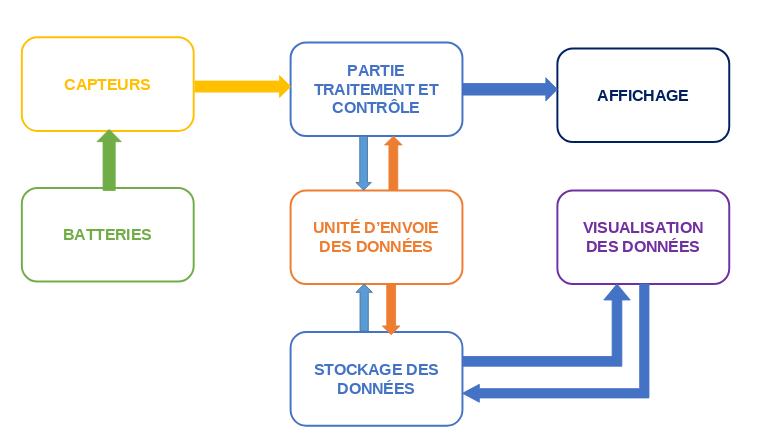
\includegraphics[width=17cm]{./img/schemaBloc.png}
	\caption{Schéma bloc du système générale }
	\label{i1}
	
\end{figure}

Le système est compose par sept bloc distinct avec leurs fonctionnement précise. Alors on va voire l'explication chaque bloc :

\paragraph{Bloc batterie : }
 celui ci est constituer par 3 batteries que le dispositif doit surveiller en temps réel.
 
\paragraph{Bloc des capteurs : }
 
Ce le bloc qui fournit les informations vers l'ensemble du systeme . Il est constitue par  des capteurs suivants :
\begin{itemize}
	\item Capteur de tension : Mesure la tension de chaque batterie.
	\item Capteur de courant : Mesure le courant de charge et de décharge de chaque batterie.
	\item	Capteur de température : Mesure la température de chaque batterie.
\end{itemize}

\paragraph{Unité de traitement et contrôle : }


Ce bloc est le cerveau de notre dispositif car il traite les informations reçues du bloc précèdent , effectuant les calculs nécessaire et convertir les données analogiques en valeurs compréhensibles par les machines, et stock les programmes nécessaires au fonctionnement du système.

\paragraph{Bloc d'affichage :}
Il est destiné a afficher les informations que le bloc precedent décide d'afficher. 

\paragraph{Unité d'envoie de données : }
il jout le role de transmission de données que le bloc de traitement a été traité et qu'il décide d'envoyer .

\paragraph{Centre de stockage  :}
Ce partie stocke les informations pré-traitées pour qu'elles puissent être utilisées pour surveiller l'état des batteries. Le stockage permet également de conserver un historique des données pour des analyses ultérieures.

\paragraph{Bloc de visualisation de données:}
C'est pour visualiser les données en temps réel que le bloc de stockage stock .

C'est une plateforme en ligne qui permet de visualiser en temps réel les tensions, courants, températures de chaque batterie ainsi que de l'ensemble du système. Cette plateforme offre également d'autres fonctionnalités comme la gestion des alertes et l'analyse des données historiques.
Pour bien comprendre l'architecture du système, la figure suivante présente une vue détaillée des composants et de leur interaction.

\begin{figure}[H]
	\centering
	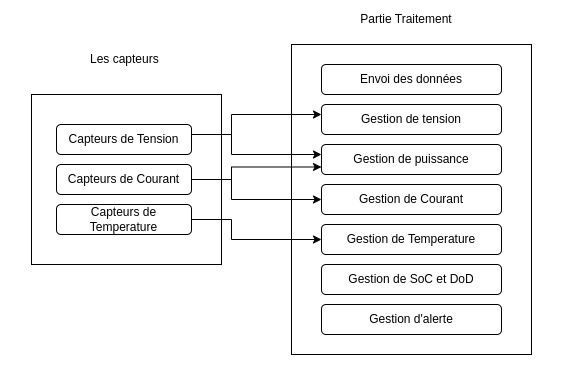
\includegraphics[width=15cm]{./img/schemaFonctionnel.png}
	\caption{Bloc de fonctionnement du système }
	\label{i1}
	
\end{figure}

\subsection*{Système de gestion de la température}
La température a une influence majeure sur le comportement de la batterie en termes de charge et de décharge. Lorsque la température baisse, la capacité de la batterie diminue également. En revanche, lorsque la température revient à la normale, la capacité retrouve son niveau habituel. À l'inverse, une augmentation de la température entraîne une augmentation de la capacité de la batterie.\\

\noindent Toutes ces variations de température affectent la durée de vie de la batterie. C'est pourquoi il est essentiel de surveiller la température de la batterie pour remédier à ces problèmes.
\\

\begin{figure}[H]
	\centering
	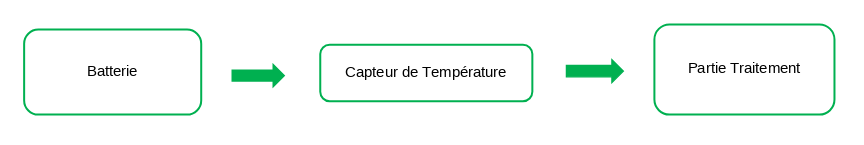
\includegraphics[width=17cm]{./img/capteurTemperature.png}
	\caption{Système de contrôle de température }
	\label{i1}
\end{figure}

Le capteur collecte les données de la batterie et vérifie d'abord si la température ne dépasse pas les seuils critiques Tcmin et Tcmax. Si ces seuils sont franchis, une alerte est envoyée à l'utilisateur.
La figure ci-dessous présente un logigramme explicatif du système.

\begin{figure}[H]
	\centering
	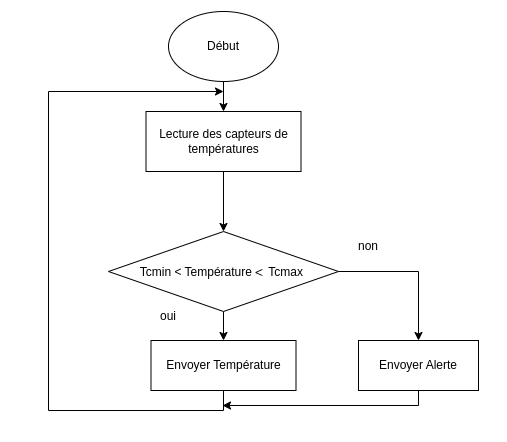
\includegraphics[width=12cm]{./img/LogigrammeDuSystemeTemperature.png}
	\caption{Logigramme du système de contrôle de température }
	\label{i1}
\end{figure}

\subsection*{Le capteur de température DS18B20} 
Le capteur thermique numérique DS18B20 est assez précise et ne nécessite aucun composant externe pour fonctionner. Il peut mesurer les températures de -55 ° C à + 125 ° C avec une précision de mesure de ± 0,5 ° C.
La résolution du capteur de mesure est configurable par l'utilisateur sur 9, 10, 11 ou 12 bits. Cependant, la résolution par défaut à la mise sous tension est de 12 bits (soit une précision de 0,0625 ° C).
\\

\noindent Cet instrument de mesure peut être alimenté avec une alimentation de 3 V à 5,5 V et ne consomme que 1 mA lors des conversions de températures actives.
\\

\noindent Voici les spécifications complètes du capteur de température numérique DS18B20: 

\begin{filleditem}
	\item Source de courant	: 3 V à 5,5 V
	\item Consommation de courant :	1mA
	\item Page de température :	-55 à 125 ° C
	\item Précision : 	± 0,5 ° C
	\item Résolution :	9 à 12 bits (sélectionnable)
	\item Temps de réponse :	<750 ms
\end{filleditem}
\begin{figure}[H]
	\centering
	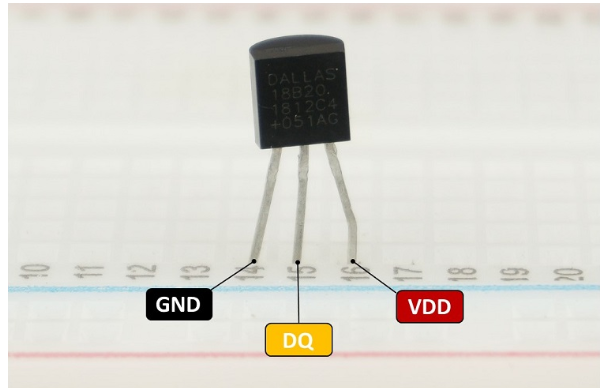
\includegraphics[width=6cm]{./img/DS18B20.png}
	\caption{Capteur de température DS18B20 }
	\label{i1}
\end{figure}

\begin{table}[H]
	\centering
	\caption{Explication des broches du DS12B20  } \vspace{5mm}
	\begin{tabular}[c]{|p{4cm}|p{10cm}|}
				
		\hline
		\rule[0.5cm]{0cm}{0cm} Noir	& GND est une broche de terre
		\\
		\hline
		\rule[0.5cm]{0cm}{0cm} Jaune &	Le DQ est un bus de données à 1 fil qui doit être connecté à une broche numérique sur le microcontrôleur.

		\\
		\hline
		\rule[0.5cm]{0cm}{0cm} Rouge &	La broche VDD fournit une alimentation au capteur qui peut être comprise entre 3,3 et 5 V.
		\\
		\hline
	
		
	\end{tabular}
\end{table}	


\subsection*{Avantage}
L'un des plus grands avantages du DS18B20 est que plusieurs DS18B20 peuvent coexister sur le même bus 1 fil. Cela signifie qu'il n'a besoin que d'une seule ligne de données (et de GND) pour communiquer avec le microcontrôleur .\\
Comme chaque DS18B20 possède un code série 64 bits unique gravé en usine, il est plus facile de les différencier les uns des autres.Cette fonctionnalité peut être un énorme avantage pour contrôler de nombreux DS18B20 répartis sur une grande surface. 
\\

Il y a deux mode que celui ci peut tirer son énergie :
\begin{itemize}
	\item une source d'alimentation externe (appelé «\textbf{ mode normale} »)
	\item la ligne de données elle-même (appelé «\textbf{ mode parasite} »), éliminant ainsi le besoin d'une alimentation externe.
\end{itemize}

\begin{figure}[H]
	\centering
	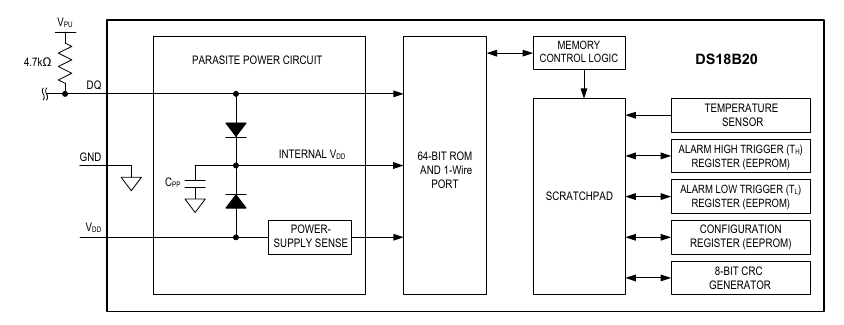
\includegraphics[width=15cm]{./img/blocDiagramDS18B20.png}
	\caption{Diagramme bloc du Capteur de température DS18B20 }
	\label{i1}
\end{figure}

\subsection*{Système de gestion de la tension et du courant}
Les batteries solaires fournissent une tension et une intensité dans une plage prédéfinie. Il est essentiel de surveiller ces paramètres en temps réel pour protéger les batteries et assurer leur bon fonctionnement. La surveillance de la tension et du courant permet également de calculer la puissance de la batterie ainsi que l'état de charge (SoC) et l'état de décharge (DoD).
\\

\begin{filleditem}
	\item \textbf{Tension} : La tension est un indicateur clé de l'état de la batterie. Une tension trop basse peut indiquer une décharge excessive, tandis qu'une tension trop élevée peut signaler une surcharge, ce qui peut endommager la batterie.
	\item	\textbf{Courant} : L'intensité du courant permet de déterminer le flux d'énergie entrant et sortant de la batterie. Des courants trop élevés peuvent surcharger la batterie, tandis que des courants trop faibles peuvent indiquer un problème de connexion ou un dysfonctionnement.
	\item	\textbf{Puissance} : La puissance fournie par la batterie est calculée à partir de la tension et du courant (P = V * I). La connaissance de la puissance permet de déterminer la capacité de la batterie à fournir de l'énergie aux charges connectées et d'optimiser l'utilisation des ressources énergétiques.
\end{filleditem}	
\subsection*{Architecture du système de gestion de la tension et du courant}
Les capteurs de tension et de courant mesurent en temps réel la tension et l'intensité de chaque batterie. Les données sont ensuite transmises au centre de traitement pour une analyse continue.

\begin{figure}[H]
	\centering
	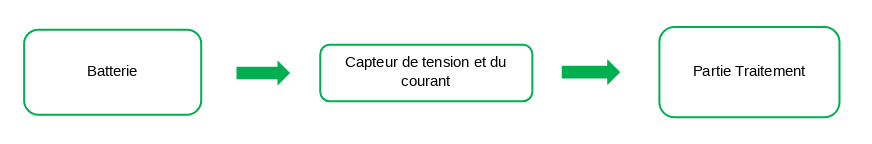
\includegraphics[width=17cm]{./img/capteurTensionCOurant.png}
	\caption{Système de contrôle de la tension et du courant }
	\label{i1}
\end{figure}

\subsection*{Module de capteur de courant continu INA226}
L'INA226 est un moniteur de courant et de tension doté d'une interface compatible I2C ou SMBUS. Il permet de surveiller à la fois la chute de tension à travers un shunt et la tension du bus d'alimentation. Grâce à une valeur d'étalonnage programmable, des temps de conversion configurables et un calcul de la moyenne, l'INA226 permet des lectures directes du courant en ampères et de la puissance en watts \cite{6}.\\

Cet appareil peut détecter le courant sur des tensions de bus allant de 0V à 36V, indépendamment de la tension d'alimentation. Il fonctionne à partir d'une seule alimentation de 2,7V à 5,5V, avec une consommation moyenne de 330 µA. L'INA226 est conçu pour une plage de températures de fonctionnement allant de -40°C à 125°C et propose 16 adresses programmables pour l'interface I2C.\\

\subsection*{Caractéristiques et spécifications}

\begin{itemize}
	\item Tension de fonctionnement : il fonctionne entre 2,7 et 5,5 volts, ce qui le rend compatible avec divers systèmes de tension.
	
	\item Plage de tension du bus : Il peut surveiller des alimentations jusqu'à 36 volts.
	
	\item Plage de détection de courant (± 500 mA à ± 50 A) : il peut surveiller une large gamme de courants en fonction de la valeur de la résistance shunt, ce qui le rend adapté à de nombreuses applications telles que la gestion de l'alimentation, les chargeurs de batterie, et le contrôle des moteurs à courant continu.
	
	\item Consommation électrique :
	\begin{itemize}
		\item  Mode continu : 0,35 mA
		\item Mode hors tension : 2,3 µA
	\end{itemize}
	
	\item Modes de mesure : Continu ou à la demande (« déclenché »)
	
	\item Moyenne des mesures : 1, 4, 64, 128, 256, 512 ou 1024 mesures individuelles
	
	\item Temps de conversion A/N réglable : Huit niveaux de 0,14 à 8,2 ms
	
	\item Précision supérieure : Grâce à son ADC 16 bits, l'INA226 offre des mesures très précises.
	
	\item Broche d'alarme programmable : Pour les violations de limites et les données disponibles. 
\end{itemize}


Le capteur possède 8 broches généralement, qui sont les suivantes :\\
\begin{figure}[H]
	\centering
	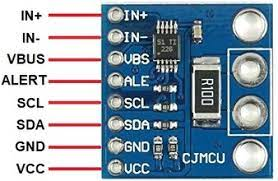
\includegraphics[width=5cm]{./img/INA226.jpeg}
	\caption{Capteur de tension et du courant INA226 }
	\label{i1}
\end{figure}

%%%\textbf{Caractéristiques principales :}
%\begin{filleditem}
%	\item Détecte les tensions de bus de 0 V à 26 V.
%	\item	Rapporte les tensions de shunt et de bus avec une haute précision.
%	\item	Précision de la tension de décalage : ± 80 µV (max).
%	\item	Erreur de gain : 0,25 % (max).
%	\item	Options de moyenne configurables.
%	\item	Quatre adresses programmables.
%	\item	Sorties d'alerte et d'avertissement programmables.
%	\item	Fonctionnement de l'alimentation : 2,7 V à 5,5 V.
%\\
%\end{filleditem}

\begin{filleditem}
	\item 	VCC : Il accepte une tension d'entrée de 2,7V à 5,5V,
	\item GND : Broche de terre, connectée à la masse de l'alimentation,
	\item SDA : Ligne de données série pour l'interface I2C. Elle est utilisée pour le transfert bidirectionnel de données,
	\item SCL : Ligne d'horloge série pour l'interface I2C. Elle est utilisée pour la synchronisation lors du transfert de données,
	\item ALE : il s'agit de la broche d'alerte,
	\item VBUS : Cette broche est utilisée pour mesurer la tension d'alimentation. Elle peut mesurer la tension d'alimentation jusqu'à 36 V,
	\item IN- : Cette broche se connecte à la charge. C'est là que la  résistance shunt est placée pour la détection du courant,
	\item IN+ : Cette broche se connecte à la source d'alimentation.\\
\end{filleditem}

%\subsection*{Avantages du INA3221}
%\begin{filleditem}
%	\item Multicanal : L'INA3221 peut surveiller simultanément la tension et le courant de trois sources distinctes, ce qui est idéal pour le projet où trois batteries solaires doivent être surveillées
	
%	\item	Efficacité : Utilisation d'un seul capteur pour plusieurs batteries réduit la complexité et le coût du système.
	
%	\item	Précision et fiabilité : Assure des mesures précises et fiables, cruciales pour la gestion optimale des batteries.
%\end{filleditem}

Le module est construit avec une puce INA226, quelques résistances et un condensateur qui aide à réduire le bruit ou les signaux électriques indésirables.

Voici le schéma du capteur :

\begin{figure}[H]
	\centering
	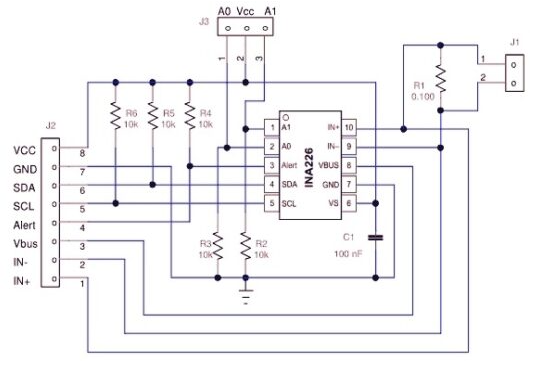
\includegraphics[width=12cm]{./img/schemabloc226.png}
	\caption{Schéma bloc de l'INA3221 }
	\label{i1}
\end{figure}


\subsection*{Système de traitement et d'envoi des données}
Le système de traitement constitue le cerveau central du système, où toutes les données capturées par les capteurs sont transmises pour être gérées, filtrées et analysées.\\
Cette phase de traitement assure plusieurs rôles cruciaux :
\begin{filleditem}
	\item \textbf{Gestion de la tension} : Contrôle des niveaux de tension pour maintenir la stabilité et éviter les surcharges ou les décharges excessives des batteries solaires.
	
	\item	\textbf{Gestion du courant} : Surveillance de courant pour optimiser l'efficacité énergétique et éviter les surcharges qui pourraient endommager les composants.
	
	\item	\textbf{Gestion de la température} : Contrôle des variations de température pour prévenir les effets néfastes sur les performances et la durée de vie des batteries.
	
	\item	\textbf{Gestion de la puissance} : Calcul et optimisation de la puissance générée et consommée par les batteries, en fonction des besoins énergétiques du système.
	
	\item	\textbf{Gestion de la charge et de la décharge} : Surveillance précise de l'état de charge (SoC) et de l'état de décharge (DoD) des batteries pour prolonger leur durée de vie et assurer une disponibilité continue.
	
	\item	\textbf{Gestion des alertes} : Détection et notification en temps réel des conditions anormales ou critiques, telles que les niveaux de tension et de température hors norme, pour permettre une intervention rapide et prévenir les défaillances potentielles.
	
	\item	\textbf{Envoi des données} : Transmission des données traitées et analysées vers une base de données en ligne ou un serveur distant, assurant ainsi une collecte centralisée et sécurisée des informations pour une surveillance continue et un suivi historique. 
\end{filleditem}

\subsection*{La carte électronique}
\subsection*{Arduino}
Arduino est une gamme de circuits électronique open source basée pour la plupart sur un micro-contrôleur du fabricant Atmel. Ces circuits intègrent les composants nécessaires pour permettre une utilisation rapide et simple du micro-contrôleur. cette simplification vise a rendre accessible à toute créations et programmation d'objet ou dispositifs interactifs . Il existe plusieurs types de carte Arduino mais pour notre cas , on va utiliser l'Arduino Mega car ce dernier comporte 16 pins analogique et 42 pins numériques. ces qui convient parfaitement au nombre des capteurs qu'on va utiliser lors de la réalisation.

\begin{figure}[H]
	\centering
	\includegraphics[width=8cm]{./img/arduinoAtmega.jpg}
	\caption{Module Arduino }
	\label{i1}
\end{figure}

\subsection*{Module GSM SIM808}

Le module est un téléphone GSM simple, sans clavier , écran , micro ni haut-parleur mais possédant une liaison série a connecter a un microcontrôleur local. Ce module prend en charge le réseau quadri bande GSM/GPRS et disponible pour la transmission et réception des SMS, de passer des appels. Ces qui fait la solution idéale de notre projet pour l'envoi des notification sous forme SMS aux utilisateur dans le cas anormaux.\\

\begin{figure}[H]
	\centering
	\includegraphics[width=6cm]{./img/gsmSim808.jpeg}
	\caption{Module GSM SIM808 }
	\label{i1}
\end{figure}

Caractéristique technique du SIM808: 
\begin{itemize}
	\item Alimentation 3,5 à 4,4 v,
	\item fréquence : 780MHz , 960MHz , 1710MHz , 2170MHz,
	\item effectuer et recevoir des appels vocaux à l'aide d'un casque et microphone externe,
	\item envoyer et recevoir des SMS,
	\item envoyer et de recevoir des données GPRS (TCP/IP , HTTP , etc),
	\item numériser et recevoir des émissions de radio FM,
	\item Dimensionnement 2.5cm x 2,3 cm x 0.7cm.
\end{itemize}


 

	\cleardoublepage
	\chapter{Transmission des données en temps réel et modélisation de l'application web}
\section{Introduction}
Dans le chapitre précédent, nous avons étudié les composants électroniques ainsi que le processus de capture des données. Dans ce chapitre, nous aborderons le principe de transmission des données en temps réel et la modélisation de l'application web, notamment la structure de la base de données qui permet de stocker les mesures traitées par le microcontrôleur. 

\subsection{Principe d'envoi des données}

Le microcontrôleur ESP32, chargé de capturer les données des capteurs (tension, courant, température), utilise son module WiFi intégré pour se connecter à Internet.

Lorsque le dispositif se trouve dans une zone couverte par un réseau WiFi, il transmet les données via ce réseau. Le protocole MQTT est utilisé pour envoyer les données capturées au serveur et à la plateforme de surveillance.

Ensuite, la plateforme et le serveur communiquent entre eux à l'aide du protocole HTTP/HTTPS pour la transmission et la récupération des données. Le serveur, quant à lui, est relié à une base de données et utilise des requêtes SQL pour la gestion et le stockage des informations.

En complément, le module GSM est réservé à l'envoi d'alertes par SMS, garantissant ainsi une communication efficace.

%Le microcontrôleur ESP32, chargé de capturer les données des capteurs (tension, courant, température), utilise un module GSM externe pour la transmission en temps réel. Ce dernier se sert du GPRS pour envoyer les informations vers un serveur en ligne, garantissant ainsi une communication efficace et fiable même sans infrastructure réseau locale.


\subsection{ WiFi intégrer au ESP32 pour la transmission des données}
Dans un environnement disposant d'un réseau WiFi, l'ESP32 se connecte directement au routeur pour transmettre les données à un serveur distant.\\

Ce schéma \ref{fig:moduleGSM1} illustre la connexion de l'ESP32 à la plateforme et au serveur, mettant en évidence les interactions entre les différents composants du système.

\begin{enumerate}
	\item \textbf{ESP32 (station WiFi)} \\
	L'ESP32, un microcontrôleur largement utilisé dans les projets IoT, se connecte à Internet via un réseau WiFi, grâce à un routeur.
	
	\item \textbf{Routeur (point d'accès)} \\
	Le routeur assure la connexion à Internet et joue le rôle de passerelle entre l'ESP32 et le serveur web.
	
	\item \textbf{Plateforme Web} \\
	La plateforme reçoit et envoie des données à l'ESP32 via le protocole MQTT. Elle publie ou s'abonne à des sujets pour faciliter la communication entre les différents composants du système.
	
	\item \textbf{Serveur Web (API REST)} \\
	Le serveur web héberge une API REST qui permet à la plateforme de soumettre et de recevoir des requêtes HTTP/HTTPS. Il agit comme une interface intermédiaire pour échanger des données avec la base de données.
	
	\item \textbf{Base de données (MySQL)} \\
	La base de données est responsable du stockage des informations collectées. Le serveur web exécute des requêtes SQL pour insérer, mettre à jour ou récupérer les données nécessaires, et transmet les résultats à la plateforme ou à l'ESP32.
\end{enumerate}


\begin{figure}[H]
	\centering
	\includegraphics[width=17cm]{./img/composants/espWIFI.png}
	\caption{Utilisation WIFI intégrer au ESP32}
	\label{fig:moduleGSM1}
\end{figure}

\textbf{Fonctionnement} : \\
L'ESP32 se connecte à Internet via un routeur WiFi, qui joue le rôle de passerelle entre l'ESP32 et le serveur web. Les données sont échangées entre la plateforme et l'ESP32 à l'aide du protocole MQTT, tandis que le serveur web utilise une API REST pour interagir avec une base de données MySQL. Cette dernière stocke et gère les informations collectées pour permettre leur consultation ou mise à jour.


\subsection{Le module GSM pour l'envoi des messages}
Connecté à l'ESP32, le module GSM permet de transmettre des alertes par SMS via le réseau cellulaire. Il est spécifiquement conçu pour informer l'utilisateur en cas de dépassement de seuils critiques, tels qu'une tension trop faible ou une surchauffe.\\

\begin{figure}[H]
	\centering
	\includegraphics[width=15cm]{./img/composants/espGSM1.png}
	\caption{Module GSM pour la transmission}
	\label{fig:moduleGSM}
\end{figure}

L'image \ref{fig:moduleGSM} montre un système de communication utilisant un module GSM pour envoyer des SMS d'alerte.

\textbf{Processus de fonctionnement :}
\begin{enumerate}
	\item \textbf{Carte SIM :} Insérée dans le module GSM pour accéder au réseau cellulaire.
	\item \textbf{Module GSM :} Reçoit des données d'un ESP32 chargé de les collecter.
	\item \textbf{Envoi de SMS :} Le module envoie des SMS d'alerte en cas de dépassement de seuils critiques.
\end{enumerate}

\textbf{Résumé :}  
L'ESP32 envoie des alertes au module GSM, qui les transmet sous forme de SMS en cas de dépassement de seuils critiques.

%\subsection{Le module GSM pour la transmission des données} Connecté à l'ESP32, le module GSM permet de transmettre les données via le réseau cellulaire. Il envoie des requêtes HTTP pour les mises à jour, et peut également transmettre des SMS d'alerte en cas de dépassement de seuils critiques (tension trop faible, surchauffe, etc.).\\

%L'image \ref{fig:moduleGSM} montre un système de communication utilisant un module GSM pour transmettre des données à une base de données via un serveur API REST.

%\textbf{Processus de fonctionnement :}
%\begin{enumerate}
%	\item \textbf{Carte SIM :} Insérée dans le module GSM pour accéder au réseau cellulaire.
%	\item \textbf{Module GSM :} Reçoit des données d'un ESP32 chargé de les collecter.
%	\item \textbf{Transmission GSM :} Le module envoie les données via le réseau cellulaire vers un serveur API REST.
%	\item \textbf{Serveur API REST :} Reçoit, interprète et traite les données.
%	\item \textbf{Requête SQL :} Le serveur envoie ensuite une requête SQL pour insérer les données dans la base de données.
%	\item \textbf{Base de données :} Stocke les données pour un accès et une analyse ultérieure.
%	\item \textbf{Notification par SMS :} Le module peut aussi envoyer des SMS à un téléphone mobile.
%\end{enumerate}

%\begin{figure}[H]
%	\centering
%	\includegraphics[width=17cm]{./img/composants/espGSM.png}
%	\caption{Module GSM pour la transmission}
%	\label{fig:moduleGSM}
%\end{figure}


%\textbf{Résumé :}  
%L'ESP32 envoie les données au module GSM, qui les transmet au serveur API REST pour traitement et stockage dans la base de données. Des SMS peuvent également être envoyés.

\subsection{Réseaux Wi-Fi }
Le \textbf{Wi-Fi} est une technologie de réseau sans fil qui utilise des fréquences radio dans les bandes de 2,4 GHz et 5 GHz pour fournir une connectivité Internet et des réseaux locaux. Elle permet la communication entre les appareils sans nécessiter de câbles, en utilisant des points d'accès (routeurs) pour transmettre les données via des ondes radio.

\subsubsection*{Fréquences}
\begin{itemize}
	\item \textbf{2,4 GHz} : Plus ancien, avec une portée plus longue mais une bande passante plus limitée et une plus grande congestion due à l'utilisation par d'autres appareils comme les téléphones sans fil et les micro-ondes.
	\item \textbf{5 GHz} : Moins encombré et offrant des vitesses de transmission plus élevées, mais avec une portée plus courte.
\end{itemize}

\subsubsection*{Débit}
Jusqu'à \textbf{600 Mbps} : débit maximal théorique selon les normes Wi-Fi, comme Wi-Fi 4 (802.11n), mais les versions plus récentes comme Wi-Fi 5 (802.11ac) et Wi-Fi 6 (802.11ax) offrent des débits beaucoup plus élevés.

\subsubsection*{Portée}
Environ \textbf{35 mètres} : portée typique en intérieur, réduite par les obstacles comme les murs épais.

\subsubsection*{Protocole}
Le Wi-Fi est un protocole \textbf{bidirectionnel}, permettant à la fois l'envoi et la réception de données, essentiel pour la mise à jour des micrologiciels et la communication entre appareils.
\subsubsection*{Avantages}
\begin{itemize}
	\item \textbf{Grande couverture} : adapté aux environnements nécessitant une large couverture, comme les bâtiments et espaces publics.
	\item \textbf{Haute vitesse} : les normes récentes (Wi-Fi 5, Wi-Fi 6) offrent des vitesses élevées, idéales pour le transfert de grandes quantités de données.
	\item \textbf{Interopérabilité} : le Wi-Fi est largement utilisé et compatible avec divers appareils et réseaux.
	\item \textbf{Coût réduit} : solution économique par rapport à d'autres protocoles sans fil.
	\item \textbf{Efficacité énergétique} : les dernières normes améliorent la gestion de l'énergie pour les dispositifs IoT.
	\item \textbf{Sécurité renforcée} : normes comme WPA3 garantissent une meilleure protection des données.
\end{itemize}


Le Wi-Fi est une technologie de communication sans fil robuste et flexible, offrant une connectivité rapide, fiable et sécurisée pour les réseaux IoT. Sa capacité à couvrir de grandes zones, sa vitesse élevée et ses fonctionnalités de sécurité en font une solution idéale pour cet projet.
\subsection{Réseau cellulaire GSM}

Le \textbf{GSM} est une norme de communication cellulaire largement utilisée pour la téléphonie mobile et les communications de données, fonctionnant sur les bandes de fréquences 900 MHz et 1800 MHz en Europe, ainsi que 850 MHz et 1900 MHz dans d'autres régions. Il offre une couverture étendue, permettant aux appareils de communiquer efficacement dans des zones urbaines et rurales.

Dans ce projet, le GSM est utilisé exclusivement pour envoyer des messages d'alerte en cas de dépassement de seuils critiques, tels qu'une tension trop faible ou une surchauffe. Grâce à sa fiabilité, le GSM garantit que les alertes par SMS parviennent à l'utilisateur, même dans des zones éloignées où d'autres options de connectivité peuvent être limitées.

\subsection*{Avantages}
\begin{itemize}
	\item \textbf{Couverture mondiale} : idéal pour les applications IoT nécessitant une portée étendue.
	\item \textbf{Interopérabilité} : compatible avec divers équipements dans différents pays.
	\item \textbf{Coût faible} : économique pour l'envoi de messages d'alerte.
	\item \textbf{Fiabilité} : technologie mature et éprouvée.
\end{itemize}

\subsection*{Inconvénients}
\begin{itemize}
	\item \textbf{Débit limité} : inadapté aux applications nécessitant des débits élevés.
	\item \textbf{Obsolescence} : en déclin avec la montée des réseaux 4G/5G.
\end{itemize}

L'utilisation du GSM dans ce projet de monitoring assure une communication fiable et économique, renforçant la capacité de surveiller les batteries solaires efficacement.

\subsection{Le protocole MQTT}  
Le protocole Message Queuing Telemetry Transport est un protocole de messagerie léger conçu pour les systèmes à ressources limitées et les communications dans des environnements où la bande passante réseau est restreinte. Il est particulièrement adapté aux applications IoT (Internet of Things) et aux dispositifs connectés nécessitant des échanges efficaces et rapides de données.  

\subsubsection{Caractéristiques principales de MQTT :}  
Le protocole MQTT repose sur le modèle \textbf{publish/subscribe (pub/sub)}, qui offre une communication flexible et asynchrone :  
\begin{itemize}  
	\item  \textbf{Publisher}  (émetteur) : envoie des messages à un ou plusieurs \textbf{topics} (sujets) spécifiques, sans se soucier des abonnés.  
	\item \textbf{Subscriber} (abonné) : s'inscrit à un ou plusieurs \textbf{topics} pour recevoir les messages publiés sur ces derniers.  
	\item \textbf{Broker} (serveur intermédiaire): joue un rôle central en agissant comme un médiateur entre les publishers et les subscribers. Il gère les abonnements, filtre les messages et distribue ceux-ci uniquement aux abonnés concernés.  


Pour la mise en œuvre, j’ai utilisé le broker open source \textbf{Mosquitto} [19], reconnu pour sa fiabilité, sa légèreté et sa compatibilité avec de nombreuses plateformes.  

\begin{figure}[H]
	\centering
	\includegraphics[width=14cm]{./img/broker.png}
	\caption{Le protocol MQTT}

\end{figure}


 	\item \textbf{Faible consommation de bande passante :}
MQTT utilise des paquets de données légers, ce qui le rend idéal pour les appareils avec une connexion réseau limitée.
\end{itemize}  
\subsection{Structure du protocole HTTP/HTTPS}

Le protocole HTTP/HTTPS repose sur un modèle client-serveur et se décompose en plusieurs éléments clés.

\subsubsection{Modèle requête-réponse}
Le protocole HTTP fonctionne selon un modèle requête-réponse, où le client envoie une requête au serveur, qui répond avec une réponse.

\subsubsection*{Requête HTTP}
Une requête HTTP se compose de trois parties :
\begin{itemize}
	\item \textbf{Ligne de requête} : contient la méthode (GET, POST, etc.), l'URL et la version du protocole. Exemple : \texttt{GET /index.html HTTP/1.1}.
	\item \textbf{En-têtes de requête} : métadonnées sur la requête. Exemple :
	\begin{verbatim}
	Host: www.example.com
	User-Agent: Mozilla/5.0
	\end{verbatim}
	\item \textbf{Corps de la requête} (facultatif) : utilisé pour les méthodes POST ou PUT. Exemple : \texttt{name=John\&age=25}.
\end{itemize}

\subsubsection*{Réponse HTTP}
Une réponse du serveur se divise en trois parties :
\begin{itemize}
	\item \textbf{Ligne de statut} : indique le résultat de la requête. Exemple : \texttt{HTTP/1.1 200 OK}.
	\item \textbf{En-têtes de réponse} : informations sur la réponse. Exemple :
	\begin{verbatim}
	Content-Type: text/html
	\end{verbatim}
	\item \textbf{Corps de la réponse} (facultatif) : contient les données demandées. Exemple :
	\begin{verbatim}
	<html><body>Welcome!</body></html>
	\end{verbatim}
\end{itemize}

\subsubsection{Méthodes HTTP}
Les principales méthodes incluent :
\begin{itemize}
	\item \textbf{GET} : récupérer une ressource.
	\item \textbf{POST} : envoyer des données au serveur.
	\item \textbf{PUT} : mettre à jour ou créer une ressource.
	\item \textbf{DELETE} : supprimer une ressource.
\end{itemize}

\subsubsection{Codes de Statut HTTP}
Les codes de statut indiquent le résultat de la requête :
\begin{itemize}
	\item \textbf{2xx (Succès)} : l'opération a réussi (ex. : 200 OK).
	\item \textbf{3xx (Redirection)} : la ressource a été déplacée (ex. : 301 Moved Permanently).
	\item \textbf{4xx (Erreur du client)} : la requête contient une erreur (ex. : 404 Not Found).
	\item \textbf{5xx (Erreur du serveur)} : le serveur a rencontré un problème (ex. : 500 Internal Server Error).
\end{itemize}

\subsubsection{HTTPS}
HTTPS est la version sécurisée de HTTP, utilisant TLS/SSL pour :
\begin{itemize}
	\item \textbf{Chiffrement} : cryptage des données échangées.
	\item \textbf{Authentification} : identification du serveur via un certificat SSL.
\end{itemize}

\subsubsection{Sessions et cookies}
HTTP est sans état, chaque requête étant indépendante. Les sessions sont gérées par des cookies, permettant de conserver des informations comme l'identifiant d'utilisateur.

\newpage
\section{ Modélisation de l'application web}
\subsection{Introduction}

Il est essentiel de modéliser les interactions entre les composants du système et les différents acteurs. À travers l'utilisation de diagrammes tels que le diagramme de cas d'utilisation, le diagramme d'activité et le diagramme de séquence, nous formaliserons le comportement, les interactions et la structure de l'application. Cette démarche vise à mieux comprendre l'architecture de l'application et à faciliter son développement.

\subsection{UML}
UML (Unified Modeling Language) est un langage standard pour modéliser les systèmes logiciels. Il propose divers diagrammes, comme le diagramme de cas d'utilisation pour représenter les interactions entre les acteurs et le système, le diagramme de séquence pour illustrer l'ordre des opérations, et le diagramme d'activité pour décrire les flux de processus. Ces outils permettent une conception claire et structurée, facilitant le développement et la maintenance des applications.
\subsubsection{Diagramme de cas d'utilisation}
Ce diagramme illustre les interactions entre les acteurs et le système, permettant de définir les fonctionnalités principales et les besoins des utilisateurs.

\begin{figure}[H]
	\centering
	\includegraphics[width=17cm]{./img/composants/diagramme/Casutilisation.png}
	\caption{Diagramme de cas d'utilisation pour l'administrateur}
\end{figure}

\subsubsection{Diagramme d'activité}
Il décrit les flux de processus sous forme d'étapes successives et de décisions, utile pour modéliser les processus métier et les scénarios complexes.
\begin{figure}[H]
	\centering
	\includegraphics[width=16cm]{./img/composants/diagramme/auth.png}
	\caption{Diagramme d'activité pour l'authentification}
\end{figure}

\begin{figure}[H]
	\centering
	\includegraphics[width=14cm]{./img/composants/diagramme/Activiter-incident.png}
	\caption{Diagramme d'activité pour la gestion de la liste des incidents}
\end{figure}
\begin{figure}[H]
	\centering
	\includegraphics[width=16cm]{./img/composants/diagramme/creationParc.png}
	\caption{Diagramme d'activité pour la création de parc}
\end{figure}

\begin{figure}[H]
	\centering
	\includegraphics[width=16cm]{./img/composants/diagramme/Activiter-plagefonctionnement.png}
	\caption{Diagramme d'activité pour la plage de fonctionnement}
\end{figure}

\begin{figure}[H]
	\centering
	\includegraphics[width=16cm]{./img/composants/diagramme/Activiter-seuilesAlerte.png}
	\caption{Diagramme d'activité pour le seuil d'alerte}
\end{figure}

\begin{figure}[H]
	\centering
	\includegraphics[width=16cm]{./img/composants/diagramme/Activiter-calendrier.png}
	\caption{Diagramme d'activité pour le calendrier de maintenance}
\end{figure}

\begin{figure}[H]
	\centering
	\includegraphics[width=16cm]{./img/composants/diagramme/Activiter-visualisation.png}
	\caption{Diagramme d'activité pour la visualisation des données}
\end{figure}








\subsubsection{Diagramme de séquence}
Ce diagramme montre l'ordre des messages échangés entre les composants ou objets d’un système, mettant en évidence la chronologie des interactions.

\begin{figure}[H]
	\centering
	\includegraphics[width=17cm]{./img/composants/diagramme/seq/1-seq-auth.png}
	\caption{Diagramme de séquence pour l'authentification}
\end{figure}


\begin{figure}[H]
	\centering
	\includegraphics[width=16cm]{./img/composants/diagramme/seq/2sequeMaintenance.png}
	\caption{Diagramme de séquence pour le calendrier de maintenance}
\end{figure}
\begin{figure}[H]
	\centering
	\includegraphics[width=17cm]{./img/composants/diagramme/seq/5seqvisualisation.png}
	\caption{Diagramme de séquence pour la visualisation des données}
\end{figure}
\begin{figure}[H]
	\centering
	\includegraphics[width=15cm]{./img/composants/diagramme/seq/parc.png}
	\caption{Diagramme de séquence pour la création de parc}
\end{figure}
\begin{figure}[H]
	\centering
	\includegraphics[width=15cm]{./img/composants/diagramme/seq/3seqyIncidentdrawio.png}
	\caption{Diagramme de séquence pour la gestion de la liste des incidents}
\end{figure}

\begin{figure}[H]
	\centering
	\includegraphics[width=15cm]{./img/composants/diagramme/seq/4seqplagefon.png}
	\caption{Diagramme de séquence pour la plage de fonctionnement}
\end{figure}
\begin{figure}[H]
	\centering
	\includegraphics[width=15cm]{./img/composants/diagramme/seq/seuil.png}
	\caption{Diagramme de séquence pour le seuil des batteries}
\end{figure}
\begin{figure}[H]
	\centering
	\includegraphics[width=17cm]{./img/composants/diagramme/seq/calendrier.png}
	\caption{Diagramme de séquence pour la calendrier de maintenance}
\end{figure}

\subsubsection{Diagramme de classe}

Un diagramme de classe UML est une représentation graphique qui illustre la structure statique d'un système. Il modélise les classes, leurs attributs, leurs méthodes (ou opérations) et les relations qui les lient.

\begin{itemize}
	\item \textbf{Nom de la classe} : il identifie la classe et se trouve dans le compartiment supérieur.
	\item \textbf{Attributs} : ce sont les propriétés ou caractéristiques d'une classe. Ils sont définis par leur visibilité, leur nom et leur type, et se placent dans le compartiment central. \\
	Exemple : \texttt{[visibilité] nomAttribut : type}.
	\item \textbf{Méthodes} : elles décrivent les comportements ou fonctionnalités d'une classe, définies par leur visibilité, leur nom, leurs paramètres et leur type de retour.
	\item \textbf{Visibilités} :
	\begin{itemize}
		\item \texttt{+} : Public,
		\item \texttt{-} : Privé,
		\item \texttt{\#} : Protégé.
	\end{itemize}
	\item \textbf{Relations} :
	\begin{itemize}
		\item \textbf{Association} : un lien entre deux classes, indiquant une interaction. La cardinalité précise le nombre d'instances impliquées (ex. : \texttt{1, 0..*, etc.}).
		\item \textbf{Héritage} : une relation où une classe dérivée hérite des propriétés et méthodes d'une classe parent.
		\item \textbf{Composition} : une relation forte où une classe fait partie intégrante d'une autre.
		\item \textbf{Agrégation} : une relation plus flexible où une classe est associée à une autre mais peut exister de façon indépendante.
		\item \textbf{Implémentation} : une classe dérivée implémente une interface.
	\end{itemize}
\end{itemize}

Dans ce projet, les diagrammes de classe ont été réalisés avec l'outil \textbf{PlantUML}, qui utilise une syntaxe textuelle simple pour créer des diagrammes. À noter que, dans PlantUML, la visibilité publique (représentée par \texttt{+} en UML standard) est affichée sous forme d'un petit rond.

Pour ce travail, les outils \textbf{UML Designer} et \textbf{PlantUML} ont été utilisés pour générer les diagrammes UML [27] [28].

\textbf{NB} : Le diagramme de classe final est présenté en annexe, au format A3.








\subsection{Draw.io}

Pour la modélisation, le logiciel libre ``Draw.io'' a été utilisé pour dessiner le diagramme de classe.

\section{Conclusion}

Dans ce chapitre, nous avons détaillé la transmission des données en utilisant le module GSM. Nous avons également abordé le protocole HTTP/HTTPS, qui s'est révélé être une solution fiable et sécurisée pour notre projet. Les données transmises sont ensuite stockées dans une base de données en ligne via une API REST, pour laquelle nous avons structuré la base afin d'assurer une gestion optimale des informations. Le prochain chapitre sera consacré à la réalisation pratique du dispositif, avec un focus sur les interfaces, les connexions et le schéma global du système.

	
	\cleardoublepage
	\chapter{Réalisation du dispositif}
\section{Introduction}
Pour réaliser le dispositif destiné à une installation de 12 kW et 400 V, nous avons rencontré des défis liés à la disponibilité des batteries et des capteurs nécessaires pour atteindre ces spécifications. Par conséquent, nous avons choisi de simuler le système à une échelle réduite en utilisant une installation domestique. Cette approche nous permet de tester les principes et le fonctionnement du système tout en réduisant le nombre de capteurs et de batteries à surveiller.

Les composants et le fonctionnement du dispositif à petite échelle sont identiques à ceux du système prévu pour 12 kW, garantissant ainsi que les résultats obtenus peuvent être extrapolés à une plus grande échelle. Cette méthode nous permet de valider le concept, d'optimiser le design, et de résoudre d'éventuels problèmes avant de passer à une installation plus importante.

\subsection{Conception et dimensionnement des divers composants du système}
L'interface de puissance dans ce projet joue un rôle crucial en gérant les interactions entre les éléments de contrôle à basse tension (comme l'ESP32) et les composants de puissance plus élevés, tels que les batteries et les relais. Elle permet d'assurer une protection efficace des composants sensibles tout en maintenant un contrôle précis des charges et de la mesure des courants, tensions et températures dans le système.

\subsubsection{Circuits de l’interface de puissance}

Le système de surveillance intègre plusieurs circuits de puissance pour gérer la charge, la décharge et la mesure des paramètres des batteries. Les relais 5V DC sont pilotés par des transistors 2N2222, car les broches de l'ESP32 ne fournissent que du 3.3V, alors que la tension d'activation des relais est de 5V. Pour la mesure de tension, des diviseurs de tension équipés de diodes Zener 1N4728A sont utilisés afin de réduire la tension et protéger les entrées du microcontrôleur. En ce qui concerne la mesure de courant, les capteurs ACS712 sont également reliés à des diviseurs de tension pour adapter la tension de sortie à un niveau acceptable pour l'ESP32.

\subsubsection*{Module relais et transistor 2N2222}

Les modules relais permettent de contrôler des charges électriques importantes en réponse aux commandes de l'ESP32. Étant donné que les sorties de l'ESP32 ne délivrent que 3.3V, des transistors 2N2222 sont utilisés comme commutateurs pour activer les relais 5V. Cette configuration permet de commuter des charges plus élevées tout en protégeant le microcontrôleur des courants et tensions élevés.

\subsubsection*{Calcul de la Résistance de Base (\(R_B\))}


\begin{figure}[H]
	\centering
	\includegraphics[width=13cm]{./img/composants/relaiset2n2222.PNG}
	\caption{Schéma du relais avec le transistor 2N2222}
	\label{fig:relais_5vdc}
\end{figure}

D’après la datasheet du transistor 2N2222 :
\begin{itemize}
	\item La tension de collecteur-émetteur en saturation (\(V_{CE_{sat}}\)) est d'environ 400 mV.
	\item Le gain minimal du transistor (\(\beta\)) est de 10.
\end{itemize}

D’après les caractéristiques du relais SONGLE SRD-05V DC SL-C :
\begin{itemize}
	\item La résistance de la bobine du relais est de 70 \(\Omega\).
	\item Alimenté par une tension \(V_{bobine} = V_{CC} - V_{CE_{sat}} = 5V - 0.4V = 4.6V\), le courant de collecteur (\(I_C\)) est donné par :
\end{itemize}

\[
I_C = \frac{V_{bobine}}{R_{bobine}} = \frac{4.6V}{70\Omega} = 0.0657A \approx 70mA
\]

Pour que le transistor fonctionne en mode commutation, il doit être saturé. Le courant de base (\(I_B\)) nécessaire est :

\[
I_B = \frac{I_C}{\beta} = \frac{70mA}{10} = 7mA
\]

La résistance de base (\(R_B\)) est calculée à partir de la tension de sortie de l'ESP32 (\(V_{GPIO}\)) et la tension de base-émetteur en saturation (\(V_{BE_{sat}}\)) du transistor :

\[
R_B = \frac{V_{GPIO} - V_{BE_{sat}}}{I_B}
\]

Avec \(V_{GPIO} = 3.3V\) et \(V_{BE_{sat}} = 0.8V\) :

\[
R_B = \frac{3.3V - 0.8V}{7mA} = \frac{2.5V}{0.007A} = 357.14 \Omega
\]

En utilisant une valeur normalisée disponible dans les séries de résistances (série E24), nous choisissons :

\[
R_B = 330 \Omega
\]
\subsubsection*{Diviseurs de tension et diode Zener 1N4728A}

Des diviseurs de tension sont utilisés pour abaisser la tension mesurée d'une batterie de 12V, qui peut atteindre jusqu'à 14.5V lorsqu'elle est complètement chargée, à des niveaux compatibles avec les entrées de l'ESP32 (3.3V). Chaque diviseur de tension est équipé d'une diode Zener 1N4728A pour protéger le microcontrôleur contre les surtensions en limitant la tension maximale appliquée aux broches de l'ESP32.

\subsubsection*{Calcul des résistances pour le diviseur de tension}
\begin{figure}[H]
	\centering
	\includegraphics[width=6cm]{./img/composants/ddt.PNG}
	\caption{Schéma du diviseur de tension avec la diode zener 1N4728A}
	\label{fig:relais_5vdc}
\end{figure}

Pour réduire une tension d'entrée de 14.5V à une tension de sortie de 3V, les valeurs des résistances du diviseur de tension sont calculées comme suit :

\[
V_{s} = V_{e} \times \frac{R_2}{R_1 + R_2}
\]

où \( V_{e} = 14.5V \) et \( V_{s} = 3V \). 

Le rapport de résistances nécessaire est :

\[
\frac{R_2}{R_1 + R_2} = \frac{V_{s}}{V_{e}} = \frac{3V}{14.5V} \approx 0.2069
\]

En choisissant \( R_1 = 4 k\Omega \) et \( R_2 = 1 k\Omega \), nous calculons la tension de sortie comme suit :

\[
V_{s} = 14.5V \times \frac{1 k\Omega}{4 k\Omega + 1 k\Omega}
\]

\[
V_{s} = 14.5V \times \frac{1}{5} = 14.5V \times 0.2 = 2.9V
\]

Avec ces valeurs, la tension de sortie est d'environ 2.9V, proche de la cible de 3V. Ce choix facilite les calculs et offre une marge de sécurité supplémentaire. En optant pour 3V au lieu de 3.3V, nous simplifions l'utilisation de résistances standards et protégeons le microcontrôleur ESP32 contre les surtensions potentielles.

\subsubsection*{Capteurs ACS712 et diviseur de tension}

Les capteurs ACS712 mesurent le courant de charge et de décharge des batteries, et leur signal de sortie doit être adapté pour correspondre à l'entrée analogique de l'ESP32. Pour ce faire, nous utilisons des diviseurs de tension.

Supposons que la sortie maximale du capteur ACS712 soit de 5V. Nous souhaitons abaisser cette tension à un niveau compatible avec l'entrée analogique de l'ESP32, qui est de 3.3V. Le choix d'une tension de sortie légèrement inférieure à 3.3V (par exemple 3V) permet d'ajouter une marge de sécurité pour protéger l'ESP32.
\begin{figure}[H]
	\centering
	\includegraphics[width=13cm]{./img/composants/ACSAVECRESISTANCE.PNG}
	\caption{Schéma du ACS712 avec le diviseur de tension}
	\label{fig:relais_5vdc}
\end{figure}

Le rapport de résistance nécessaire est calculé comme suit :

\[
\frac{R_2}{R_1 + R_2} = \frac{V_{s}}{V_{e}} = \frac{3V}{5V} = 0.6
\]

Pour atteindre ce rapport avec des valeurs standard de résistances, nous choisissons \( R_1 \) et \( R_2 \). Supposons que nous choisissons \( R_2 = 2k\Omega \). Nous pouvons alors calculer \( R_1 \) en utilisant la formule :

\[
\frac{R_2}{R_1 + R_2} = 0.6 \implies R_1 + R_2 = \frac{R_2}{0.6}
\]

\[
R_1 = \frac{R_2}{0.6} - R_2 = \frac{2k\Omega}{0.6} - 2k\Omega = \frac{2000}{0.6} - 2000 \approx 3333 - 2000 = 1333 \Omega
\]

Nous choisissons alors la valeur standard la plus proche, \( R_1 = 1k\Omega \), et recalculons la tension de sortie :

\[
V_{s} = V_{e} \times \frac{R_2}{R_1 + R_2} = 5V \times \frac{2k\Omega}{1k\Omega + 2k\Omega} = 5V \times \frac{2}{3} \approx 3.33V
\]

Cette tension est légèrement au-dessus de 3.3V, offrant ainsi une marge de sécurité. Les valeurs choisies permettent d'adapter efficacement le signal de sortie du capteur à l'entrée de l'ESP32 tout en utilisant des résistances standards facilement disponibles.

\subsubsection{Brochage des Composants}
\subsubsection*{Relais}
\begin{table}[H]
	\centering
	\caption{Brochage des Relais}
	\begin{tabular}{|p{4.5cm}|p{3.5cm}|p{2cm}|p{3.5cm}|}
		\hline
		\rule[0.5cm]{0cm}{0cm} \textbf{Relais} & \textbf{GND} & \textbf{VCC} & \textbf{IN} \\
		\hline
		\rule[0.5cm]{0cm}{0cm} Relais 1 & GND de l'ESP32 & 5V & GPIO 5 \\
		\hline
		\rule[0.5cm]{0cm}{0cm} Relais 2 & GND de l'ESP32 & 5V & GPIO 18 \\
		\hline
		\rule[0.5cm]{0cm}{0cm} Relais 3 & GND de l'ESP32 & 5V & GPIO 19 \\
		\hline
		\rule[0.5cm]{0cm}{0cm} Relais 4 & GND de l'ESP32 & 5V & GPIO 23 \\
		\hline
	\end{tabular}
\end{table}

\subsubsection*{Capteurs de Courant (ACS712)}

\begin{table}[H]
	\centering
	\caption{Brochage des Capteurs de Courant (ACS712)}
	\begin{tabular}{|p{5.5cm}|p{2cm}|p{3.5cm}|p{2.5cm}|}
		\hline
		\rule[0.5cm]{0cm}{0cm} \textbf{Capteur} & \textbf{VCC} & \textbf{GND} & \textbf{OUT} \\
		\hline
		\rule[0.5cm]{0cm}{0cm} ACS712 pour Batterie 1 & 5V & GND de l'ESP32 & GPIO 36 \\
		\hline
		\rule[0.5cm]{0cm}{0cm} ACS712 pour Batterie 2 & 5V & GND de l'ESP32 & GPIO 39 \\
		\hline
		\rule[0.5cm]{0cm}{0cm} ACS712 pour Batterie 3 & 5V & GND de l'ESP32 & GPIO 25 \\
		\hline
		\rule[0.5cm]{0cm}{0cm} ACS712 pour Courant Global & 5V & GND de l'ESP32 & GPIO 26 \\
		\hline
	\end{tabular}
\end{table}

\subsubsection*{Capteurs de Température (LM35)}

\begin{table}[H]
	\centering
	\caption{Brochage des Capteurs de Température (LM35)}
	\begin{tabular}{|p{4.5cm}|p{2cm}|p{3.5cm}|p{3.5cm}|}
		\hline
		\rule[0.5cm]{0cm}{0cm} \textbf{Capteur} & \textbf{VCC} & \textbf{GND} & \textbf{OUT} \\
		\hline
		\rule[0.5cm]{0cm}{0cm} LM35 pour Batterie 1 & 5V & GND de l'ESP32 & GPIO 34 \\
		\hline
		\rule[0.5cm]{0cm}{0cm} LM35 pour Batterie 2 & 5V & GND de l'ESP32 & GPIO 35 \\
		\hline
		\rule[0.5cm]{0cm}{0cm} LM35 pour Batterie 3 & 5V & GND de l'ESP32 & GPIO 32 \\
		\hline
	\end{tabular}
\end{table}

\subsubsection*{Diviseurs de Tension}

\begin{table}[H]
	\centering
	\caption{Brochage des Diviseurs de Tension}
	\begin{tabular}{|p{6.5cm}|p{1.5cm}|p{3.5cm}|p{2cm}|}
		\hline
		\rule[0.5cm]{0cm}{0cm} \textbf{Diviseur de Tension} & \textbf{VCC} & \textbf{GND} & \textbf{OUT} \\
		\hline
		\rule[0.5cm]{0cm}{0cm} Diviseur de Tension pour Batterie 1 & 12V & GND de l'ESP32 & GPIO 33 \\
		\hline
		\rule[0.5cm]{0cm}{0cm} Diviseur de Tension pour Batterie 2 & 12V & GND de l'ESP32 & GPIO 27 \\
		\hline
		\rule[0.5cm]{0cm}{0cm} Diviseur de Tension pour Batterie 3 & 12V & GND de l'ESP32 & GPIO 14 \\
		\hline
		\rule[0.5cm]{0cm}{0cm} Diviseur de Tension pour Batterie Globale & 12V & GND de l'ESP32 & GPIO 12 \\
		\hline
	\end{tabular}
\end{table}

\subsubsection*{Afficheur LCD I2C}

\begin{table}[H]
	\centering
	\caption{Brochage de l'Afficheur LCD I2C}
	\begin{tabular}{|p{4.5cm}|p{2cm}|p{3cm}|p{2cm}|p{2cm}|}
		\hline
		\rule[0.5cm]{0cm}{0cm} \textbf{Afficheur LCD I2C} & \textbf{VCC} & \textbf{GND} & \textbf{SDA} & \textbf{SCL} \\
		\hline
		\rule[0.5cm]{0cm}{0cm} Afficheur LCD I2C & 5V & GND de l'ESP32 & GPIO 21 & GPIO 22 \\
		\hline
	\end{tabular}
\end{table}

\subsubsection*{Module GSM}

\begin{table}[H]
	\centering
	\caption{Brochage du Module GSM}
	\begin{tabular}{|p{4.5cm}|p{2cm}|p{3cm}|p{2cm}|p{2cm}|}
		\hline
		\rule[0.5cm]{0cm}{0cm} \textbf{Module GSM} & \textbf{VCC} & \textbf{GND} & \textbf{RX} & \textbf{TX} \\
		\hline
		\rule[0.5cm]{0cm}{0cm} Module GSM & 5V & GND de l'ESP32 & GPIO 17 & GPIO 16 \\
		\hline
	\end{tabular}
\end{table}

\subsubsection*{Leds}
\begin{table}[H]
	\centering
	\caption{Brochage des leds}
	\begin{tabular}{|p{4.5cm}|p{3.5cm}|p{3.5cm}|}
		\hline
		\rule[0.5cm]{0cm}{0cm} \textbf{Led} & \textbf{GND} & \textbf{OUT} \\
		\hline
		\rule[0.5cm]{0cm}{0cm} Led pour le gsm 1 & GND de l'ESP32  & GPIO 4 \\
		\hline
	\end{tabular}
\end{table}


\begin{landscape}
\begin{figure}[]
	\centering
	\includegraphics[width=25cm]{./img/schema22.PNG}
	\caption{Schéma d'ensemble du système}
	\label{fig:relais_5vdc}
\end{figure}
\end{landscape}

\subsection{Câblage réalisé}
Tous les composants électroniques ont été montés et soudés sur une plaquette perforée à l'aide de fil bobine pour les liaisons. Seuls les capteurs de température nécessitent l'utilisation de connecteurs USB mâles/femelles pour assurer leur connexion avec le dispositif, tandis que les capteurs de tension et de courant sont directement reliés au système de surveillance des batteries solaires.

\begin{figure}[H]
	\centering
	\includegraphics[width=10cm]{./img/composants/realisation.png}

	\label{fig:relais_5vdc}
\end{figure}
\begin{figure}[H]
	\centering
	\includegraphics[width=10cm]{./img/composants/realisationDos.png}
		\caption{Câblage des composantes}
	\label{fig:relais_5vdc}
\end{figure}

\subsection{Mise en boîte}
Dimensionner et concevoir le boîtier afin d'accueillir les composants déjà câblés, notamment le port USB femelle, l'écran LCD, l'antenne, la puce GSM, les LED et les fixations des fils reliés aux batteries, tout en prenant en compte les contraintes de taille et d'accessibilité pour une utilisation optimale.

\begin{figure}[H]
	\centering
	\includegraphics[width=17cm]{./img/dispo3.png}
\caption{Mise en boîte du dispositif}
\end{figure}
\begin{figure}[H]
	\centering
	\includegraphics[width=4cm]{./img/cable.png}
\caption{Câbles avec connecteur USB mâle pour les capteurs LM35}

\end{figure}

\section{Conclusion}

Ce chapitre a permis d'explorer le dimensionnement des composants essentiels en calculant leurs valeurs, ainsi que d'examiner les interfaces de puissance et les brochages entre le microcontrôleur ESP32 et les autres composants qui lui sont reliés. La présentation du câblage a illustré comment chaque élément s'assemble pour former un système cohérent et fonctionnel. Ces connaissances constituent une base solide pour les étapes suivantes de notre projet, y compris la réalisation du tableau de bord, ainsi que l'implémentation et les tests.


	
	\cleardoublepage
	\chapter{Présentation des interfaces}
\section{Introduction}
Dans ce chapitre, nous présenterons les différentes interfaces du tableau de bord, ainsi que les technologies utilisées pour leur conception et leur mise en œuvre.

\subsection{Technologies utilisées}

La création de la plateforme est divisée en deux parties principales : le \textbf{frontend} et le \textbf{backend}, chacune reposant sur des technologies spécifiques pour répondre aux besoins fonctionnels et assurer une expérience utilisateur optimale.

\subsubsection{Frontend}
\begin{itemize}
	\item \textbf{Vue.js 3} : Framework JavaScript moderne utilisé pour construire une interface utilisateur réactive et performante [20].
	\item \textbf{Pinia} : Bibliothèque de gestion d'état utilisée pour centraliser et organiser les données de manière efficace [21].
	\item \textbf{Axios} : Utilisé pour établir une communication entre le frontend et le backend via des requêtes HTTP (API REST) [22].
	\item \textbf{MQTT} : Protocole léger utilisé pour les communications en temps réel, permettant de s'abonner aux topics générés par le dispositif pour recevoir des données instantanées [23].
\end{itemize}

\subsubsection{Backend}
\begin{itemize}
	\item \textbf{Laravel} : Framework PHP robuste permettant de développer des API backend performantes et sécurisées [24].
	\item \textbf{MySQL} : Base de données relationnelle utilisée pour stocker et gérer les données de manière structurée et efficace [25].
\end{itemize}

\subsubsection{Gestion des versions}
\begin{itemize}
	\item \textbf{GitHub} : Plateforme utilisée pour le contrôle de version, facilitant la gestion collaborative du projet et le suivi des modifications apportées au code source [26].
\end{itemize}

\section{Les interfaces }

\subsection{Authentification}

Cette page d’authentification, utilisée par tous les utilisateurs de l'application \textbf{BatMonitor}, permet de gérer l'accès à la plateforme de manière sécurisée. Le nom BatMonitor a été choisi pour refléter la vocation principale de l'application : le suivi et le monitoring en temps réel des batteries solaires.

Pour se connecter, l’utilisateur doit entrer son email et son mot de passe, puis cliquer sur le bouton\textbf{ Se connecter}.
S’il souhaite créer un compte, il doit cliquer sur \textbf{S'inscrire}.


\begin{figure}[H]
	\centering
	\includegraphics[width=17cm]{./img/interface/login.png}
	\caption{Authentification ( se connecter)}
	\label{fig:relais_5vdc}
\end{figure}

\begin{figure}[H]
	\centering
	\includegraphics[width=17cm]{./img/interface/singup.png}
	\caption{Authentification (S'inscrire)}
	\label{fig:relais_5vdc}
\end{figure}

\subsection{Page d'accueil}

Cette page permet de visualiser en temps réel les données de chaque batterie, telles que la tension, le courant, la température, ainsi que les graphiques correspondants. Les options de navigation disponibles dépendent du rôle de l'utilisateur. En cliquant sur le bouton \textbf{Détail}, il est possible d'accéder à des informations plus approfondies sur chaque batterie.

\begin{figure}[H]
	\centering
	\includegraphics[width=17cm]{./img/Interfaces/acceuil.png}
	\caption{Page d'accueil}
	\label{fig:relais_5vdc}
\end{figure}

\begin{figure}[H]
	\centering
	\includegraphics[width=17cm]{./img/interface/detailAcceuil.png}
	\caption{Page détail de batterie}
	\label{fig:relais_5vdc}
\end{figure}

\subsection{Page de gestion du parc}

En accédant à la section \textbf{Gestion du parc} via le menu de navigation, l'utilisateur peut créer un parc, consulter, modifier, visualiser les détails ou supprimer un parc existant. La page dédiée au calendrier de maintenance permet de visualiser les maintenances récentes ainsi que l'historique des interventions. Il est également possible de supprimer ou de modifier la description d'une maintenance.
 
\begin{figure}[H]
	\centering
	\includegraphics[width=17cm]{./img/Interfaces/gestionParcCreation.png}
	\caption{Gestion de parc sur la création parc}
	\label{fig:relais_5vdc}
\end{figure}


\begin{figure}[H]
	\centering
	\includegraphics[width=17cm]{./img/Interfaces/gestionParcMaintenance.png}
	\caption{Gestion de parc sur la calendrier de maintenance}
	\label{fig:relais_5vdc}
\end{figure}

\subsection{Paramètres de la batterie}

Cette section permet de consulter les plages de fonctionnement de chaque batterie en affichant tous les paramètres détaillés. En accédant à la section \textbf{Seuils d'alerte}, il est possible de visualiser les seuils de fonctionnement spécifiques à chaque batterie.



\begin{figure}[H]
	\centering
	\includegraphics[width=17cm]{./img/interface/PlageFonctionement.png}
	\caption{Paramètres de la batterie sur la plage de fonctionnement}
	\label{fig:relais_5vdc}
\end{figure}

\begin{figure}[H]
	\centering
	\includegraphics[width=17cm]{./img/interface/seuilAlerte.png}
	\caption{Paramètres de la batterie sur la seuil d'alerte}
	\label{fig:relais_5vdc}
\end{figure}


\subsection{Page de gestion des incidents}

Cette page permet de consulter la liste des incidents récents ainsi que l'historique des incidents. Il est possible d'effectuer une recherche par date via le champ de recherche. En cliquant sur le bouton \textbf{Récent}, les incidents récents s'affichent, tandis que le bouton \textbf{Historique} permet de visualiser les incidents passés.

\begin{figure}[H]
	\centering
	\includegraphics[width=17cm]{./img/interface/listeIncident.png}
	\caption{Page de gestion des incidents sur récent}
	\label{fig:relais_5vdc}
\end{figure}



\subsection{Page d'historique des données}

Cette page permet de visualiser les données stockées sous forme de graphiques, affichant la tension, le courant et la température de chaque batterie en fonction de l'historique des données : jour, semaine, mois ou année.

\begin{figure}[H]
	\centering
	\includegraphics[width=17cm]{./img/interface/visualisationDonne.png}
	\caption{Page d'historique des données}
	\label{fig:relais_5vdc}
\end{figure}

\subsection{Notifications}

En cliquant sur l'icône cloche, l'utilisateur peut accéder aux notifications.

\begin{figure}[H]
	\centering
	\includegraphics[width=17cm]{./img/interface/notification.png}
	\caption{Notification}
	\label{fig:relais_5vdc}
\end{figure}
\section{Conclusion}

En résumé, le système de gestion et de surveillance développé permet un suivi en temps réel des batteries, offrant une vue d'ensemble précise de leurs paramètres de fonctionnement tels que la tension, le courant et la température. Grâce à l'interface utilisateur intuitive, les utilisateurs peuvent facilement accéder aux informations essentielles, consulter l'historique des données, et gérer les incidents et maintenances avec efficacité. La mise en place des fonctionnalités de notifications et d'alertes assure une réactivité accrue face aux éventuels dysfonctionnements. 



	
	\cleardoublepage
	\chapter{Traitement des données et conception de l'intelligence artificielle}

\section{Introduction}
Dans le chapitre précédent, nous avons exploré la création d'une plateforme de visualisation des données. Ce chapitre se concentre sur le traitement des données collectées et la conception d'un modèle d'intelligence artificielle. Nous détaillerons les étapes nécessaires pour préparer les données, sélectionner et optimiser le modèle, et évaluer ses performances. L'objectif est de rendre les données exploitables pour l'entraînement du modèle et d'assurer une prédiction précise des paramètres clés des batteries.

\subsection{Traitement des données}
\subsubsection{Collecte des données}
Il est essentiel de normaliser les données collectées, car elles peuvent contenir du bruit. Les données brutes mesurées sont les suivantes :
\begin{itemize} 
	\item La tension 
	\item Le courant 
	\item La température
	\item SoC
	\item DoD
 \end{itemize}

Pour obtenir ces données, nous avons réalisé une collecte durant un cycle de charge et de décharge d'une batterie Lithium NMC-LCO 18650, d'une capacité nominale de 2,8 Ah et d'une tension nominale de 3,7 V, en appliquant un courant de charge et de décharge. Les caractéristiques complètes de la batterie se trouvent dans l'annexe. 

Les données collectées sont transmises par l'ESP32 et stockées dans la base de données pour être visualisées et utilisées par la plateforme, ainsi que pour la prédiction et l'entraînement du modèle. Voici, dans cette image, un aperçu de la table qui contient les données :

\begin{figure}[H]
	\centering
	\includegraphics[width=17cm]{./img/tableLecture.png}
	\caption{Table dans la base de données ( Lectures )}
\end{figure}

\subsubsection{Nettoyage des données}
Les données brutes collectées peuvent contenir des erreurs, des incohérences ou des valeurs aberrantes dues à des défauts des capteurs, des interférences environnementales ou des problèmes de communication. Ces erreurs peuvent fausser les analyses, les prévisions et les conclusions tirées.

Définir une plage nominale afin de filtrer les valeurs qui se trouvent en dehors de ces limites.



\begin{table}[H]
	\centering
	\caption{Plage des valeurs acceptables}
	\begin{tabular}{|p{5cm}|p{5cm}|}
		\hline
		\textbf{Paramètre} & \textbf{Plage} \\
		\hline
		Tension & 2.75V - 4.2V \\
		\hline
		Courant & 1.4A - 4.2A \\
		\hline
		Température & 0°C à 60°C \\
		\hline
		SOC & 0\% à 100\% \\
		\hline
		DOD & 0\% à 100\% \\
		\hline
	\end{tabular}
\end{table}

Les données manquantes peuvent provenir de pannes de capteurs, interruptions réseau ou autres problèmes techniques. Pour y remédier, plusieurs méthodes sont utilisées :

\subsubsection{Gestion des valeurs manquantes}

\begin{itemize}
	\item \textbf{Imputation (remplacement des valeurs manquantes)}
	\begin{itemize}
		\item \textbf{Moyenne / Médiane (Température des batteries) :} Remplace une valeur manquante par la moyenne ou médiane des valeurs voisines.
		
		\textbf{Exemple :} Si la température à $t = 10s$ est absente, elle est estimée par la moyenne des valeurs à $t = 9s$ et $t = 11s$.
		
		\item \textbf{Interpolation (Tension et courant) :} Estime une valeur manquante à partir des mesures avant et après.
		
		\textbf{Exemple :} Si la tension à $t = 6s$ est absente, elle peut être estimée par une interpolation linéaire entre $3.3V$ ($t = 5s$) et $3.5V$ ($t = 7s$), donnant :
		
		\[
		V(6s) = \frac{3.3V + 3.5V}{2} = 3.4V
		\]
	\end{itemize}
	
	\item \textbf{Suppression des données incomplètes}
	
	Si plus de 50\% des données sont manquantes, l’enregistrement est supprimé pour éviter les biais.
	
	\textbf{Exemple :} Un SoC mesuré sur 10 instants, dont 6 valeurs sont manquantes, est jugé non fiable et ignoré.
	
	\item \textbf{Réduction du bruit et détection des anomalies}
	\begin{itemize}
		\item \textbf{Filtre de Kalman (Tension et courant) :} Lisse les variations et améliore la précision des mesures.
		
		\textbf{Exemple :} Si la tension passe brutalement de $3.5V$ à $10V$, le filtre corrige cette incohérence en tenant compte des valeurs précédentes.
	\end{itemize}
\end{itemize}
\subsection{Définition des nouveaux paramètres}
Les nouveaux paramètres sont obtenus grâce à des méthodes de traitement des données et des calculs spécifiques, également connus sous le nom d'ingénierie des features. Ces paramètres sont particulièrement adaptés pour l'entraînement de modèles et la prédiction des performances des batteries, en permettant une analyse plus approfondie de leur comportement au cours des cycles de charge et de décharge.

\begin{table}[H]
	\centering
	\caption{Définition des nouveaux paramètres}
	\begin{tabular}{|p{6cm}|p{9cm}|}
		\hline
		\textbf{Paramètre} & \textbf{Description} \\
		\hline
		\textbf{Cycle} & Nombre de cycles complets de charge et de décharge effectués par la batterie \\
		\hline
		\textbf{Temps de décharge/charge} & Durée totale des phases de charge et de décharge (en secondes) \\
		\hline
		\textbf{Tension de décharge/charge} & Tension mesurée pendant la phase de charge ou de décharge \\
		\hline
		\textbf{Courant de décharge/charge} & Courant circulant lors des phases de charge et de décharge \\
		\hline
		\textbf{Tension max. en décharge (V)} & Tension maximale atteinte au cours de la décharge \\
		\hline
		\textbf{Tension min. en charge (V)} & Tension minimale atteinte au cours de la charge \\
		\hline
		\textbf{RUL} & Estimation de la durée de vie restante de la batterie \\
		\hline
		\textbf{SOH} & Indicateur de l'état de santé de la batterie, exprimant son efficacité par rapport à sa capacité initiale \\
		\hline
		\textbf{Température de décharge/charge} & Température de la batterie durant les cycles de charge et de décharge \\
		\hline
	\end{tabular}
\end{table}


\subsubsection*{Identifier les cycles de charge/décharge}
Un cycle de charge/décharge est défini comme une décharge complète suivie d'une recharge complète. On détecte un cycle en surveillant le SoC :

\begin{itemize}
	\item Décharge : \textbf{SoC diminue} de \textbf{100\%} vers \textbf{20\%} (ou un seuil bas défini).
	\item Charge : \textbf{SoC remonte} à \textbf{100\%}.
\end{itemize}

\subsubsection*{Calcul du temps de charge et de décharge}
\begin{itemize}
	\item \textbf{Temps de décharge} = Durée entre SoC\_max et SoC\_min.
	\item \textbf{Temps de charge} = Durée entre SoC\_min et SoC\_max.
\end{itemize}

\subsubsection*{Extraction de la tension min/max lors de la charge et de la décharge}
\begin{itemize}
	\item \textbf{Max Voltage en décharge} = Valeur maximale atteinte lors de la phase de décharge.
	\item \textbf{Min Voltage en charge} = Valeur minimale atteinte lors de la phase de charge.
\end{itemize}

%\subsubsection*{Calcul du temps en courant constant}
%Lors de la charge, le \textbf{courant reste constant} pendant un moment avant de diminuer (phase de saturation).

\subsubsection*{Calcul de la Capacité Actuelle}  
La capacité actuelle est obtenue en intégrant le courant de charge et de décharge au cours du temps :  

\begin{equation}
C_{\text{actuelle}} = C_{\text{initiale}} - \int I_{\text{décharge}}(t) \, dt
\end{equation}

où :  
\begin{itemize}
	\item $C_{\text{initiale}}$ est la capacité nominale de la batterie (en Ah),
	\item $I_{\text{décharge}}(t)$ est le courant de décharge instantané (en A),
	\item $dt$ est l'intervalle de temps de mesure.
\end{itemize}

En pratique, l'intégration est souvent effectuée de manière discrète par un microcontrôleur :  

\begin{equation}
C_{\text{actuelle}} = C_{\text{initiale}} - \sum I_{\text{décharge}}(t) \times \Delta t
\end{equation}

avec $\Delta t$ en heures pour que le résultat soit en Ah.

\subsubsection*{Estimation de la durée de vie restante (RUL)}
La \textbf{RUL} est une estimation du nombre de cycles restants avant la fin de vie de la batterie. Elle est basée sur la \textbf{capacité de la batterie} et son \textbf{taux de dégradation}.

\begin{equation}
RUL = \left( \frac{C_{\text{actuelle}}}{C_{\text{initiale}}} \right) \times \text{Nombre\_de\_cycles}
\end{equation}

où $\text{Nombre\_de\_cycles}$ représente le nombre total de cycles que la batterie peut supporter avant d'atteindre un seuil critique de capacité (par exemple, 80 \% de $C_{\text{initiale}}$).

\subsubsection*{Calcul du SOH (State of Health)}
Le \textbf{SOH}) mesure la capacité actuelle de la batterie par rapport à sa capacité initiale. Il est généralement exprimé en pourcentage et permet d’évaluer l'état de santé de la batterie.

\begin{equation}
SOH = \left( \frac{C_{\text{actuelle}}}{C_{\text{initiale}}} \right) \times 100
\end{equation}

Un \textbf{SOH de 100 \%} signifie que la batterie est en parfait état, tandis qu’un \textbf{SOH de 80 \% ou moins} indique une batterie vieillissante nécessitant un remplacement prochain.


\section{Modélisation} 
\subsection{Description des modèles}

Il existe plusieurs modèles que l'on peut explorer en Machine Learning, mais nous allons nous concentrer sur quelques-uns parmi les plus couramment utilisés, à savoir :

\begin{itemize}
	\item \textbf{Régression linéaire} : Modèle simple établissant une relation linéaire entre variables indépendantes et dépendante.
	\item \textbf{Régression de crête} : Variante de la régression linéaire avec pénalité L2 pour réduire la complexité et éviter le sur-apprentissage.
	\item \textbf{Régression Lasso} : Similaire à la régression de crête, mais avec pénalité L1, permettant la sélection automatique des caractéristiques.
	\item \textbf{Forêt aléatoire} : Ensemble d'arbres de décision réduisant le sur-apprentissage tout en maintenant une grande précision.
	\item \textbf{K-Plus proches voisins} : Modèle basé sur la proximité des données, avec la sortie déterminée par les k voisins les plus proches.
	\item \textbf{Réseaux de neurones artificiels} : Modèles inspirés du cerveau humain, capables de modéliser des relations complexes via des couches successives de neurones.
\end{itemize}

\subsubsection{R\'egression lin\'eaire (Linear Regression)}

La r\'egression lin\'eaire est un mod\`ele simple et largement utilis\'e en apprentissage automatique. Elle vise \`a mod\'eliser la relation entre une ou plusieurs variables ind\'ependantes \(X\) et une variable d\'ependante \(Y\) en ajustant une droite (ou un hyperplan en dimension sup\'erieure) minimisant l'erreur quadratique. L'\'equation du mod\`ele est :

\begin{equation}
Y = \beta_0 + \beta_1 X_1 + \beta_2 X_2 + \dots + \beta_n X_n
\end{equation}
O\`u :
\begin{itemize}
	\item \( Y \) : variable d\'ependante (valeur \`a pr\'edire).
	\item \( X_1, X_2, \dots, X_n \) : variables ind\'ependantes (pr\'edictives).
	\item \( \beta_0 \) : ordonn\'ee \`a l'origine.
	\item \( \beta_1, \beta_2, \dots, \beta_n \) : coefficients du mod\`ele \`a estimer.
\end{itemize}

\textbf{Avantages :}
\begin{itemize}
	\item Facile \`a impl\'ementer et interpr\'eter.
	\item Convient aux donn\'ees lin\'eairement s\'eparables.
	\item Exige peu de ressources de calcul.
\end{itemize}

\subsubsection{R\'egression de cr\^ete (Ridge Regression)}

La r\'egression de cr\^ete introduit une p\'enalit\'e L2 pour r\'eduire le sur-apprentissage en contraignant la magnitude des coefficients. La fonction de co\^ut devient :

\begin{equation}
J(\beta) = \sum_{i=1}^{m} (y_i - \hat{y}_i)^2 + \lambda \sum_{j=1}^{n} \beta_j^2
\end{equation}
O\`u :
\begin{itemize}
	\item \( y_i \) : valeur r\'eelle de l'observation \(i\).
	\item \( \hat{y}_i \) : valeur pr\'edite.
	\item \( \lambda \) : param\`etre de r\'egularisation (contr\^ole la p\'enalit\'e).
	\item \( \beta_j \) : coefficients du mod\`ele.
\end{itemize}

\textbf{Avantages :}
\begin{itemize}
	\item R\'eduit le risque de sur-apprentissage.
	\item Convient aux donn\'ees ayant de fortes corr\'elations entre les variables.
\end{itemize}

\subsubsection{R\'egression Lasso (Lasso Regression)}

La r\'egression Lasso applique une p\'enalit\'e L1, ce qui permet la s\'election de variables en annulant certains coefficients. La fonction de co\^ut est :


\begin{equation}
\hat{C} = \sum_{i=1}^{m} (y_i - \hat{y}_i)^2 + \lambda \sum_{j=1}^{n} |\beta_j|
\end{equation}

\textbf{Avantages :}
\begin{itemize}
	\item Permet la s\'election automatique des variables les plus importantes.
	\item R\'eduit la complexit\'e du mod\`ele en mettant certains coefficients \`a z\'ero.
\end{itemize}

\subsubsection{For\^et al\'eatoire (Random Forest)}

La for\^et al\'eatoire est un mod\`ele d'ensemble bas\'e sur plusieurs arbres de d\'ecision. Chaque arbre est entra\^in\'e sur un sous-ensemble al\'eatoire du jeu de donn\'ees. La pr\'ediction finale est obtenue par agr\'egation :



\begin{equation}
\hat{y} = \frac{1}{n_{arbres}} \sum_{i=1}^{n_{arbres}} f_i(X)
\end{equation}

\textbf{Avantages :}
\begin{itemize}
	\item Pr\'ecision \'elev\'ee et robuste \`a l'overfitting.
	\item Convient aux relations non lin\'eaires.
	\item G\'ere les donn\'ees bruit\'ees et les valeurs manquantes.
\end{itemize}

\subsubsection{K-Plus Proches Voisins (K-Nearest Neighbors, KNN)}

KNN pr\'edit une valeur en utilisant les \(K\) plus proches voisins d'un point dans l'espace des caract\'eristiques. Pour une r\'egression, la pr\'ediction est la moyenne :

\begin{equation}
\hat{y} = \frac{1}{K} \sum_{i=1}^{K} y_i
\end{equation}
\textbf{Avantages :}
\begin{itemize}
	\item Simple \`a comprendre et \`a impl\'ementer.
	\item Fonctionne bien pour des donn\'ees locales complexes.
	\item Pas besoin d'hypoth\`ese sur la distribution des donn\'ees.
\end{itemize}

\subsubsection{R\'eseaux de neurones artificiels (Artificial Neural Networks, ANN)}

Les r\'eseaux de neurones sont compos\'es de couches de neurones interconnect\'es. Chaque neurone applique une fonction d'activation \`a une somme pond\'er\'ee des entr\'ees :

\begin{equation}
Z^{(l)} = W^{(l)} a^{(l-1)} + b^{(l)}
\end{equation}

\begin{equation}
a^{(l)} = f(Z^{(l)})
\end{equation}



\textbf{Avantages :}
\begin{itemize}
	\item Excellente capacit\'e \`a mod\'eliser des relations non lin\'eaires complexes.
	\item Adapt\'e aux grands jeux de donn\'ees et aux probl\`emes multi-dimensionnels.
	\item Am\'eliorable avec des techniques comme le deep learning.
\end{itemize}


\subsection{Critères d'évaluation des modèles de régression}

\subsubsection{Erreur Quadratique Moyenne (MSE)}
\begin{equation}
MSE = \frac{1}{n} \sum_{i=1}^{n} (y_i - \hat{y}_i)^2
\end{equation}
\textbf{Interprétation :} 

Plus la valeur du MSE est faible, plus le modèle est précis. Cependant, il est très sensible aux valeurs aberrantes, car il élève les erreurs au carré.
\begin{itemize}
	\item MSE = 0 : modèle parfait, aucune erreur.
	\item MSE > 0 : le modèle présente des erreurs, avec une erreur plus grande pour des valeurs plus élevées.
\end{itemize}

\subsubsection{Erreur Absolue Moyenne (MAE)}
\begin{equation}
MAE = \frac{1}{n} \sum_{i=1}^{n} |y_i - \hat{y}_i|
\end{equation}
\textbf{Interprétation :} 

Le MAE représente l'erreur moyenne en valeur absolue. Il est moins sensible aux valeurs aberrantes que le MSE, mais ne met pas autant en évidence les grandes erreurs.
\begin{itemize}
	\item MAE = 0 : modèle parfait, aucune erreur.
	\item MAE > 0 : le modèle présente des erreurs proportionnelles à la magnitude de l'erreur absolue.
\end{itemize}

\subsubsection{Erreur Quadratique Moyenne Racine (RMSE)}
\begin{equation}
RMSE = \sqrt{MSE} = \sqrt{\frac{1}{n} \sum_{i=1}^{n} (y_i - \hat{y}_i)^2}
\end{equation}
\textbf{Interprétation :} 

Le RMSE permet d'obtenir une erreur moyenne dans la même unité que la variable cible, facilitant son interprétation par rapport au MSE.
\begin{itemize}
	\item RMSE = 0 : modèle parfait, aucune erreur.
	\item RMSE > 0 : le modèle présente des erreurs, et plus la valeur est grande, plus les erreurs sont importantes.
\end{itemize}

\subsubsection{Coefficient de Détermination ($R^2$)}
\begin{equation}
R^2 = 1 - \frac{\sum (y_i - \hat{y}_i)^2}{\sum (y_i - \bar{y})^2}
\end{equation}
\textbf{Interprétation :} 

Le $R^2$ indique la proportion de la variance expliquée par le modèle. Une valeur proche de 1 signifie que le modèle ajuste bien les données, tandis qu'une valeur proche de 0 indique un faible pouvoir explicatif.
\begin{itemize}
	\item $R^2 = 1$ : modèle parfait, explique toute la variance des données.
	\item $R^2 = 0$ : le modèle n'offre aucune amélioration par rapport à la moyenne, il n'explique aucune variance.
	 \item $R^2 < 0$ : la prédiction est inférieure à la moyenne, les résultats sont moins précis que la simple moyenne des valeurs cibles.
\end{itemize}


\subsection{Validation des modèles de régression}

\subsubsection{Validation croisée (Cross-Validation)}
\textbf{Principe :} la validation croisée consiste à diviser l'ensemble de données en plusieurs sous-ensembles ou "folds". À chaque itération, un sous-ensemble est utilisé comme jeu de test, tandis que les autres sous-ensembles servent à l'entraînement du modèle. Cette procédure permet de mesurer la performance du modèle de manière plus robuste, en réduisant le risque de surapprentissage (overfitting).
\begin{itemize}
	\item \textbf{k-Fold Cross-Validation :} diviser l'ensemble de données en $k$ sous-ensembles égaux, puis entraîner le modèle $k$ fois, chaque fois en utilisant un sous-ensemble différent comme jeu de test. L'erreur moyenne sur les $k$ itérations est calculée comme suit :
	
	\begin{equation}
	\text{Score moyen} = \frac{1}{K} \sum_{k=1}^{K} \text{Score}_k
	\end{equation}
	où :
	\begin{itemize}
		\item $K$ : représente le nombre total de plis (ou "folds") dans la validation croisée.
		\item $\text{Score}_k$ : représente le score de performance pour le $k$-ième pli.
		\item Les données sont divisées en $K$ sous-ensembles égaux.
		\item Le modèle est entraîné sur $K-1$ sous-ensembles et testé sur le sous-ensemble restant.
		\item Ce processus est répété $K$ fois, chaque sous-ensemble servant de test une fois.
		\item Le score moyen est calculé en prenant la moyenne des scores de performance obtenus sur chaque pli.
	\end{itemize}
	
%	\subsubsection*{Time Series Split :}
%	\begin{itemize}
%		\item Adapté aux séries temporelles, où les données sont divisées en plis successifs en respectant l'ordre chronologique.
%		\item Cela évite la contamination des données de test par les données futures.
%		\item Le score moyen est calculé de manière similaire en prenant la moyenne des scores de performance pour chaque pli, en respectant l'ordre temporel.
%	\end{itemize}

\end{itemize}

\subsubsection{Courbe d'apprentissage}
\textbf{Principe :} les courbes d'apprentissage permettent de suivre l'évolution de la performance du modèle au fur et à mesure de l'entraînement. Elles sont particulièrement utiles pour détecter les problèmes de surapprentissage ou de sous-apprentissage.
\begin{itemize}
	\item \textbf{Surapprentissage (Overfitting) :} si la performance du modèle sur le jeu d'entraînement continue de s'améliorer tandis que celle sur le jeu de test se dégrade, cela indique un surapprentissage.
	\item \textbf{Sous-apprentissage (Underfitting) :} si le modèle ne parvient pas à bien ajuster à la fois le jeu d'entraînement et le jeu de test, cela peut indiquer un sous-apprentissage, où le modèle est trop simple pour capturer les relations dans les données.
\end{itemize}

\subsubsection{Évaluation sur un jeu de test indépendant}
\textbf{Principe :} après avoir entraîné le modèle sur un sous-ensemble des données (jeu d'entraînement), il est important d'évaluer sa performance sur un jeu de test indépendant qui n'a pas été utilisé pendant l'entraînement. Cela permet de s'assurer que le modèle est capable de généraliser et de faire des prédictions fiables sur des données non vues.
\begin{itemize}
	\item Un jeu de test indépendant permet d'éviter le biais d'évaluation dû au surapprentissage sur les données d'entraînement.
\end{itemize}


\section{Développement et implémentation}
 \subsection{Outils} Durant le développement, en particulier pour le traitement des données, l'entraînement et le test du modèle, nous avons utilisé la plateforme en ligne Google Colab, qui est gratuite. Elle facilite l'installation des frameworks et des bibliothèques nécessaires au développement, telles que :

\begin{itemize} 
	\item pandas 
	\item NumPy 
	\item Scikit-learn 
	\item TensorFlow 
	\item Keras 
\end{itemize}

\section{Phases de prédiction}

L'objectif est de créer un modèle entraîné capable de prédire les paramètres suivants : 
\begin{itemize} 
	\item SOH : état de santé de la batterie 
	\item RUL : nombre de cycles restants de la batterie \end{itemize}

Voici l'organigramme illustrant le processus de prédiction : 


\begin{figure}[H]
	\centering
	\includegraphics[width=12cm]{./img/processus.png}
	\caption{Organigramme du processus de prédiction}

\end{figure}


\subsection{Acquisition des données}

Nous importons le fichier "battery\_data\_collecter.csv" ici pour pouvoir l'utiliser dans notre travail.

\begin{minted}[frame=single,framesep=8pt]{python}

from google.colab import files
uploaded = files.upload() 
data = pd.read_csv('battery_data_collecter.csv')
print(data.head())

\end{minted}

\textbf{Résultats}
\begin{figure}[H]
	\centering
	\includegraphics[width=16cm]{./img/resultats/loadData.png}
    \caption{Affichage du résultat du chargement des données collectées brutes}

\end{figure}


\subsection{Nettoyage des données}
Suppression des valeurs manquantes et des doublons, suivie de l’élimination des valeurs aberrantes à l’aide de la méthode de l’écart interquartile (IQR).
\begin{minted}[frame=single,framesep=8pt]{python}

# Fonction pour identifier et filtrer les valeurs aberrantes
def remove_outliers(df):
   for column in df.select_dtypes(include=[np.number]).columns:
     Q1 = df[column].quantile(0.25)
     Q3 = df[column].quantile(0.75)
     IQR = Q3 - Q1
     lower_bound = Q1 - 1.5 * IQR
     upper_bound = Q3 + 1.5 * IQR
     # Filtrer les valeurs aberrantes
     df = df[(df[column] >= lower_bound) & (df[column] <= upper_bound)]
   return df
	
# 1. Suppression des valeurs manquantes
data_cleaned = data.dropna()
	
# 2. Suppression des doublons
data_cleaned = data_cleaned.drop_duplicates()
	
# 3. Identification et traitement des valeurs aberrantes
data_cleaned = remove_outliers(data)
	
# Vérifier la structure des données après nettoyage
print(data_cleaned.describe())
\end{minted}
\textbf{Résultats}
\begin{figure}[H]
	\centering
	\includegraphics[width=16cm]{./img/resultats/netoyage.png}
	\caption{Affichage du résultat du nettoyage des données brutes collectées}
	
\end{figure}
\subsection{Transformation des données}
Les données sont transformées et normalisées afin d'obtenir de nouveaux paramètres essentiels pour le dataset, garantissant une meilleure qualité des données d'entraînement.
\begin{minted}[ frame=single, fontsize=\small, breaklines]{python}

#Transformation des Données
def calculate_cycle_summary(df, capacity_nominal, life_cycle_nominal=500):
  # Extraire les valeurs nécessaires du DataFrame
  soc_values = df['SOC (%)'].values
  timestamps = df['Timestamp (s)'].values
  tensions = df['Tension (V)'].values
  currents = df['Courant (A)'].values
  temperatures = df['Température (°C)'].values
  
  # Initialiser les variables pour le calcul
  total_discharge = 0
  charge_time = 0
  discharge_time = 0
  charge_tensions, discharge_tensions = [], []
  charge_currents, discharge_currents = [], []
  charge_temperatures, discharge_temperatures = [], []
  	
  # Parcourir les valeurs de SOC pour déterminer les phases de charge et de décharge
  for i in range(1, len(soc_values)):
    delta_soc = soc_values[i] - soc_values[i - 1]
    delta_time = timestamps[i] - timestamps[i - 1]
    
    if delta_soc > 0:  # Phase de charge
      charge_time += delta_time
      charge_tensions.append(tensions[i])
      charge_currents.append(currents[i])
      charge_temperatures.append(temperatures[i])
    elif delta_soc < 0:  # Phase de décharge
      discharge_time += delta_time
      total_discharge += abs(delta_soc)
      discharge_tensions.append(tensions[i])
      discharge_currents.append(currents[i])
      discharge_temperatures.append(temperatures[i])
  
  # Calculer le nombre total de cycles
  total_cycles = total_discharge / 100
  
  # Calculer les moyennes des tensions, courants et températures pendant les phases de charge et décharge
  avg_v_charge = sum(charge_tensions) / len(charge_tensions) if charge_tensions else 0
  avg_v_discharge = sum(discharge_tensions) / len(discharge_tensions) if discharge_tensions else 0
  avg_i_charge = sum(charge_currents) / len(charge_currents) if charge_currents else 0
  avg_i_discharge = sum(discharge_currents) / len(discharge_currents) if discharge_currents else 0
  avg_t_charge = sum(charge_temperatures) / len(charge_temperatures) if charge_temperatures else 0
  avg_t_discharge = sum(discharge_temperatures) / len(discharge_temperatures) if discharge_temperatures else 0
  
  # Trouver les valeurs maximales et minimales de tension pendant les phases de charge et décharge
  max_v_discharge = max(discharge_tensions) if discharge_tensions else 0
  min_v_charge = min(charge_tensions) if charge_tensions else 0
  	
  # Convertir le temps de décharge en heures
  discharge_time_h = discharge_time / 3600
  capacity_discharged = avg_i_discharge * discharge_time_h
  
  # Calculer le State of Health (SOH)
  soh = (capacity_discharged / (capacity_nominal * total_cycles)) * 100 if capacity_nominal and total_cycles > 0 else 0
  
  # Calculer le Remaining Useful Life (RUL)
  rul = (life_cycle_nominal * soh / 100) - total_cycles if total_cycles > 0 else life_cycle_nominal
  
  # Créer un DataFrame de résumé avec les résultats calculés
  summary_df = pd.DataFrame({
  	'Cycles': [total_cycles],
  	'T_charge (s)': [charge_time],
  	'T_discharge (s)': [discharge_time],
  	'V_charge (V)': [avg_v_charge],
  	'V_discharge (V)': [avg_v_discharge],
  	'V_max_dis (V)': [max_v_discharge],
  	'V_min_chg (V)': [min_v_charge],
  	'I_charge (A)': [avg_i_charge],
  	'I_discharge (A)': [avg_i_discharge],
  	'T°C_charge': [avg_t_charge],
  	'T°C_discharge': [avg_t_discharge],
  	'SOH (%)': [soh],
  	'RUL (cycles)': [rul]
  })
  return summary_df
\end{minted}


\subsection{Séparation des données}
Les données sont divisées en un ensemble d'entraînement (80 \%) et un ensemble de test (20 \%).
\begin{minted}[ frame=single, fontsize=\small, breaklines]{python}

  # Préparation des données pour l'entraînement et la normalisation
  # Séparation des variables cibles (RUL et SOH)
  y_rul = df['RUL (cycles)']
  y_soh = df['SOH (%)']
  
  # Suppression des colonnes cibles du jeu de données pour obtenir
   les entrées (features)
  x = df.drop(columns=['RUL (cycles)', 'SOH (%)'], axis=1)
  
  # Division des données en ensembles d'entraînement et de test (80% entraînement, 20% test)
  x_train, x_test, y_train_rul, y_test_rul = train_test_split(x, y_rul, test_size=0.20, random_state=42)
  _, _, y_train_soh, y_test_soh = train_test_split(x, y_soh, test_size=0.20, random_state=42)
  
  # Normalisation des données pour améliorer la performance des modèles
  scaler = StandardScaler()
  x_train = scaler.fit_transform(x_train)
  x_test = scaler.transform(x_test)
\end{minted}


\subsection{Sélection du modèle}
Lister les modèles sélectionnés pour l'entraînement, en les entraînant un par un afin de pouvoir comparer leurs performances.
\begin{minted}[ frame=single, fontsize=\small, breaklines]{python}

   # Définition d'un dictionnaire contenant différents modèles de régression
   
   models = {
   	# Régression linéaire simple
   	"Linear Regression": LinearRegression(),
   	# Régression Ridge avec régularisation 
   	"Ridge Regression": Ridge(alpha=0.1, random_state=42),
   	 # Régression Lasso avec régularisation
   	"Lasso Regression": Lasso(alpha=0.001, random_state=42)
   	# Modèle Random Forest optimisé 
   	"Random Forest (Optimized)": best_rf,
   	# Régression par plus proches voisins (KNN)
   	"K-Nearest Neighbors": KNeighborsRegressor(),
   	# Régression par réseau de neurones artificiels (MLP)  
   	"ANN Regression": MLPRegressor(hidden_layer_sizes=(256,), max_iter=1000, random_state=42)  
   }
\end{minted}


\subsection{Optimisation des hyperparamètres}
Ajustement des paramètres du modèle à l'aide de GridSearch, en définissant le nombre d'arbres, la profondeur maximale et le nombre minimal d'échantillons requis pour diviser un nœud.
\begin{minted}[ frame=single, fontsize=\small, breaklines]{python}

   # Recherche d'hyperparamètres avec GridSearchCV pour Random Forest
   # Définition des hyperparamètres à tester
   rf_params = {
   	'n_estimators': [50, 100, 200],  # Nombre d'arbres dans la forêt
   	'max_depth': [10, 20, None],  # Profondeur maximale des arbres
   	'min_samples_split': [2, 5, 10]  # Nombre minimum d'échantillons pour diviser un nœud
   }
   
   # Initialisation du modèle Random Forest
   rf = RandomForestRegressor(random_state=42)
   
   # GridSearchCV pour rechercher la meilleure combinaison d'hyperparamètres
   grid_search_rf = GridSearchCV(rf, rf_params, cv=5, scoring='r2', n_jobs=-1)
   
   # Entraînement du modèle avec GridSearchCV
   grid_search_rf.fit(x_train, y_train_rul)
   
   # Récupération du meilleur modèle après recherche des hyperparamètres
   best_rf = grid_search_rf.best_estimator_
   
   # Affichage des meilleurs hyperparamètres trouvés
   print(f"Meilleurs hyperparamètres pour Random Forest : {grid_search_rf.best_params_}")
\end{minted}
Affichage de résultat : 
\begin{figure}[H]
	\centering
	\includegraphics[width=16cm]{./img/resultats/goodParam.png}
	\caption{ Affichage des meilleurs hyperparamètres trouvés}
	
\end{figure}


\subsection{Entraînement du modèle}
Entraînement des modèles sur l'ensemble de données d'entraînement afin d'ajuster leurs paramètres et optimiser leurs performances.
\begin{minted}[frame=single, fontsize=\small, breaklines]{python}

   # Entraînement et évaluation des modèles
   # Liste pour stocker les résultats de performance des modèles
   results = []
   
   # Parcours de chaque modèle défini dans le dictionnaire "models"
   for name, model in models.items():
     # ----------------------
     # Entraînement et évaluation pour RUL (Remaining Useful Life)
     # ----------------------
     
     model.fit(x_train, y_train_rul)
     
     # Prédictions sur les ensembles d'entraînement et de test
     y_pred_train_rul = model.predict(x_train)
     y_pred_test_rul = model.predict(x_test)
     
     # Calcul des métriques de performance pour RUL
     metrics_rul = calculate_metrics(y_train_rul, y_test_rul, y_pred_train_rul, y_pred_test_rul)
     
     # Ajout d'informations sur le modèle et la cible dans les résultats
     metrics_rul['Model'] = name
     metrics_rul['Target'] = 'RUL (cycles)'
     
     # Validation croisée pour évaluer la robustesse du modèle
     metrics_rul['CrossVal R2'] = cross_val_score_model(model, x, y_rul)
     
     # Stockage des résultats pour RUL
     results.append(metrics_rul)
     
     # Enregistrement du modèle entraîné pour RUL
     joblib.dump(model, f'{name}_rul_model.pkl')
   
     # ----------------------
     # Entraînement et évaluation pour SoH (State of Health)
     # ----------------------
     
	 model.fit(x_train, y_train_soh)
	    
     # Prédictions sur les ensembles d'entraînement et de test
     y_pred_train_soh = model.predict(x_train)
     y_pred_test_soh = model.predict(x_test)
     
     # Calcul des métriques de performance pour SoH
     metrics_soh = calculate_metrics(y_train_soh, y_test_soh, y_pred_train_soh, y_pred_test_soh)
     
     # Ajout d'informations sur le modèle et la cible dans les résultats
     metrics_soh['Model'] = name
     metrics_soh['Target'] = 'SOH (%)'
     
     # Validation croisée pour évaluer la robustesse du modèle
     metrics_soh['CrossVal R2'] = cross_val_score_model(model, x, y_soh)
     
     # Stockage des résultats pour SoH
     results.append(metrics_soh)
     
     # Enregistrement du modèle entraîné pour SoH
     joblib.dump(model, f'{name}_soh_model.pkl')
   
   # Conversion des résultats en DataFrame pour une meilleure visualisation
   results_df = pd.DataFrame(results)
	
   # Affichage des résultats des modèles
   print("Résultats des modèles :\n", results_df)
\end{minted}


\subsection{Validation du modèle}
Évaluation du modèle à l'aide de techniques de validation croisée.
\begin{minted}[ frame=single, fontsize=\small, breaklines]{python}

	# Validation croisée pour évaluer le modèle
	def cross_val_score_model(model, x, y):
	scores = cross_val_score(model, x, y, cv=5, scoring='r2')
	return np.mean(scores)
\end{minted}

\subsection{Génération des prédictions}
Utilisation du modèle pour produire des prédictions.
\begin{minted}[ frame=single, fontsize=\small, breaklines]{python}

   # Normalisation des nouvelles données
   new_data_scaled = scaler.transform(new_data)
   
   # Stockage des prédictions
   predictions = []
   
   # Prédiction avec chaque modèle
   for name in models.keys():
      model_rul = joblib.load(f'{name}_rul_model.pkl')
      prediction_rul = model_rul.predict(new_data_scaled)
      
      model_soh = joblib.load(f'{name}_soh_model.pkl')
      prediction_soh = model_soh.predict(new_data_scaled)
      
      predictions.append({
      	'Model': name,
      	'Predicted RUL': prediction_rul[0],
      	'Predicted SoH': prediction_soh[0]
      })
   
   # Conversion en DataFrame et affichage
   predictions_df = pd.DataFrame(predictions)
   print("Prédictions :\n", predictions_df)
\end{minted}


\subsection{Évaluation des prédictions}
Mesure de la performance du modèle avec des métriques telles que MAE, RMSE et $R^2$.
\begin{minted}[ frame=single, fontsize=\small, breaklines]{python}

   # Fonction de calcul des métriques d'évaluation
   def calculate_metrics(y_train, y_test, y_pred_train, y_pred_test):
     return {
     	'MAE Train': mean_absolute_error(y_train, y_pred_train),
     	'MSE Train': mean_squared_error(y_train, y_pred_train),
     	'R2 Train': r2_score(y_train, y_pred_train),
     	'MAE Test': mean_absolute_error(y_test, y_pred_test),
     	'MSE Test': mean_squared_error(y_test, y_pred_test),
     	'R2 Test': r2_score(y_test, y_pred_test)
   }
\end{minted}


\subsection{Analyse des résultats}

Voici les images des résultats des métriques pendant l'entraînement et le test, suivies de la validation croisée.
\begin{figure}[H]
	\centering
	\includegraphics[width=17cm]{./img/resultats/Train.png}
	\caption{Résultats des métriques d'entraînement}
	\label{fig:train_metrics}
\end{figure}

\begin{figure}[H]
	\centering
	\includegraphics[width=17cm]{./img/resultats/train.png}
	\caption{Résultats des métriques de test et de validation croisée}
	\label{fig:test_validation_metrics}
\end{figure}

\subsubsection{Interprétation des résultats}

\subsubsection*{Prédiction du RUL (cycles)}
\begin{itemize}
	\item \textbf{Régressions linéaires (Linear, Ridge, Lasso) :} très bonnes performances avec $R^2 \approx 0.99951$, mais des erreurs (MAE, MSE) légèrement plus élevées que Random Forest.
	\item \textbf{Random Forest :} meilleure précision avec $R^2 = 0.99998$ et des erreurs extrêmement faibles.
	\item \textbf{K-Nearest Neighbors (KNN) :} performance inférieure avec $R^2 = 0.99808$ et des erreurs plus élevées.
	\item \textbf{ANN Regression :} bonne performance ($R^2 = 0.99951$), mais erreurs plus élevées que Random Forest.
\end{itemize}

\subsubsection*{Prédiction du SOH (\%)}
\begin{itemize}
	\item \textbf{Régressions linéaires :} similaires à RUL avec de très bonnes performances ($R^2 \approx 0.99951$), mais inférieures à Random Forest.
	\item \textbf{Random Forest :} meilleure précision avec $R^2 = 0.99998$ et des erreurs très faibles.
	\item \textbf{KNN :} performance inférieure avec $R^2 = 0.99808$ et erreurs plus élevées.
	\item \textbf{ANN Regression :} bonne capacité de prédiction ($R^2 = 0.99944$), mais moins précise que Random Forest.
\end{itemize}

\subsubsection*{Validation croisée}
\begin{itemize}
	\item \textbf{Random Forest :} excellente généralisation avec $R^2 = 0.99925$.
	\item \textbf{ANN Regression :} résultats incohérents en validation croisée, nécessitant une vérification.
\end{itemize}

\begin{itemize}
	\item \textbf{Random Forest est le modèle le plus performant} avec les meilleures valeurs de $R^2$ et les erreurs les plus faibles.
	\item \textbf{Les modèles de régression linéaire} sont solides mais légèrement moins précis.
	\item \textbf{KNN a les performances les plus faibles}, tandis qu'\textbf{ANN regression présente des résultats incohérents en validation croisée}.
\end{itemize}




\subsection{Visualisation des prédictions}
Création de graphiques pour visualiser les prédictions de consommation sur différentes périodes.
\begin{minted}[linenos, frame=single, fontsize=\small, breaklines]{python}

   # Visualisation des performances
   plt.figure(figsize=(12, 6))
   for target in ['RUL (cycles)', 'SOH (%)']:
     subset = results_df[results_df['Target'] == target]
     for metric in ['R2 Train', 'R2 Test', 'CrossVal R2']:
        plt.barh(subset['Model'], subset[metric], label=f'{metric} {target}')
   plt.title("Comparaison des performances des modèles")
   plt.xlabel("Score")
   plt.legend()
   plt.show()
\end{minted}

\subsection{Choix du model}
Le modèle \textbf{Random Forest} a été choisi pour plusieurs raisons clés, basées sur ses performances supérieures :

\subsubsection*{Performance}
\begin{itemize}
	\item \textbf{R² élevé} : le R² est très élevé pour l'entraînement et les tests, indiquant une forte capacité de prédiction pour RUL et SOH.
	\item \textbf{Faibles erreurs} : les erreurs absolue (MAE) et quadratique (MSE) sont faibles, surtout pour SOH, montrant des prédictions fiables.
\end{itemize}

\subsubsection*{Généralisation}
\begin{itemize}
	\item \textbf{Validation croisée} : le R² de validation croisée est élevé (0.99925), indiquant une bonne généralisation et minimisant le sur-apprentissage.
\end{itemize}

\subsubsection*{Comparaison avec d'autres modèles}
\begin{itemize}
	\item \textbf{Précision supérieure} : comparé à la régression linéaire et Ridge, Random Forest a une meilleure précision avec des MAE et MSE plus faibles pour RUL.
	\item \textbf{Meilleure performance} : par rapport à KNN et ANN, Random Forest a des erreurs plus faibles et une meilleure précision, notamment pour RUL.
\end{itemize}

\subsubsection*{Robustesse}
\begin{itemize}
	\item \textbf{Ensemble d'arbres} : random Forest est robuste aux variations de données et aux valeurs aberrantes, grâce à sa structure d'ensemble d'arbres de décision.
\end{itemize}
En résumé, \textbf{Random Forest} est préféré pour sa capacité à généraliser, ses faibles erreurs de prédiction, et ses excellentes performances en termes de R².
\section{Intégration}

Après avoir sélectionné le modèle optimal pour la prédiction du SOH et du RUL, nous téléchargeons les modèles entraînés :  

\begin{minted}[ frame=single, fontsize=\small, breaklines]{python}
   from google.colab import files
   
   # Télécharger les modèles entraînés depuis Google Colab
   files.download('Random Forest_rul_model.pkl')
   files.download('Random Forest_soh_model.pkl')
\end{minted}

Ensuite, nous transférons ces modèles vers le serveur hébergeant notre backend Laravel. Un script est mis en place pour exécuter les modèles et traiter les prédictions. De plus, un contrôleur spécifique et une route API dédiée sont implémentés pour intégrer ces prédictions au sein du système.  


\section{Conclusion}
Ce chapitre a exploré le traitement des données et la conception d'un modèle d'intelligence artificielle pour prédire le RUL et le SOH des batteries. Nous avons nettoyé et transformé les données, puis évalué plusieurs modèles de régression, notamment la régression linéaire, Ridge, Lasso, Random Forest, K-Nearest Neighbors, et les réseaux de neurones artificiels.

Le modèle Random Forest s'est distingué par ses performances supérieures, avec des valeurs de R² élevées et des erreurs faibles. Il a également montré une excellente capacité de généralisation grâce à la validation croisée.





























	
	\cleardoublepage
	\cleardoublepage
\markboth{Conclusion générale et perspectives}{Conclusion générale et perspectives} % Ajout de la commande \markboth
\chapter*{Conclusion générale et perspectives}
\addcontentsline{toc}{chapter}{Conclusion générale et perspectives}

Au terme de notre étude sur le système de surveillance des batteries solaires, nous avons mis en lumière l'importance cruciale des systèmes photovoltaïques et des nombreux facteurs influençant leur performance. La qualité des panneaux solaires, des batteries et des autres équipements, ainsi qu'un dimensionnement approprié, sont essentiels pour garantir un fonctionnement optimal. La nécessité d'une surveillance régulière des paramètres tels que la température, la tension et le courant a été soulignée, démontrant l'importance d'un dispositif de monitoring efficace.

Nous avons également exposé le principe de fonctionnement de notre dispositif, en mettant en avant la sélection minutieuse des composants électroniques. Chaque élément a été choisi en fonction de ses caractéristiques techniques et de son adéquation avec les exigences de notre système de surveillance, ce qui est fondamental pour assurer la fiabilité de l'ensemble.

La transmission des données a été détaillée en utilisant le Wi-Fi, les protocoles HTTP/HTTPS ainsi que le protocole MQTT, garantissant une communication sécurisée entre le dispositif et la plateforme, tout en assurant une transmission efficace vers une base de données en ligne. Par ailleurs, nous avons procédé à la modélisation de la base de données en concevant une structure optimisée sous MySQL pour le stockage des données collectées, ce qui facilite l'accès et l'analyse des informations.

Le dimensionnement des composants et les connexions entre le microcontrôleur ESP32 et les autres éléments du système ont également été explorés, illustrant la cohérence du système. Ces connaissances constituent une base solide pour les prochaines étapes, notamment la réalisation du tableau de bord et l'implémentation des tests.

En perspectives, nous envisageons d'approfondir l'analyse des données recueillies pour optimiser encore davantage la gestion des batteries solaires. De plus, l'ajout de fonctionnalités intelligentes, comme la prédiction des performances basées sur l'historique des données, pourrait enrichir notre système. Enfin, des tests sur le terrain permettront de valider l'ensemble des performances et d'ajuster le dispositif selon les besoins spécifiques des utilisateurs.

	
	
	
	\pagenumbering{roman}
	\cleardoublepage
	\renewcommand{\bibname}{Bibliographie}
	\bibliographystyle{unsrt}
	\bibliography{references}
	\addcontentsline{toc}{chapter}{Webographie}
\chapter*{Webographie}
\noindent [5] MESupReS, \textbf{C'est quoi LMD ?}, http://lmd.mesupres.gov.mg/?page=lmd, du 2014.  \\

\noindent [6] https://fr.wikipedia.org/wiki/Representational\_state\_transfer \\


\noindent [7] https://dev.mysql.com/doc/\\

\noindent [8] https://www.fluter.dev\\

\noindent [9] https://www.php.net\\

\noindent [9] https://www.apachefriends.org\\


	
	\cleardoublepage
	\fancyhead[L]{Annexe}
	\chapter*{Annexe}
\phantomsection
\addcontentsline{toc}{chapter}{Annexe}

\appendix
\section*{Extrais du code SQL des tables}

\noindent CREATE TABLE `parcs` (\\
	`id` bigint(20) UNSIGNED NOT NULL,\\
	`nom\_parc` varchar(255) NOT NULL,\\
	`description` varchar(255) NOT NULL,\\
	`adresse` varchar(255) NOT NULL,\\
	`nombre\_batteries` varchar(255) NOT NULL,\\
	`user\_id` bigint(20) UNSIGNED NOT NULL,\\
	`systeme\_parametre\_id` bigint(20) UNSIGNED NOT NULL,\\
	`created\_at` timestamp NULL DEFAULT NULL,\\
	`updated\_at` timestamp NULL DEFAULT NULL\\
	) ENGINE=InnoDB DEFAULT CHARSET=utf8mb4 COLLATE=utf8mb4\_unicode\_ci;\\

\noindent CREATE TABLE `batteries` (\\
`id` bigint(20) UNSIGNED NOT NULL,\\
`nom` varchar(255) NOT NULL,\\
`capacite\_nominal` varchar(255) NOT NULL,\\
`date\_installation` date NOT NULL,\\
`technologie` varchar(255) NOT NULL,\\
`marque` varchar(255) NOT NULL,\\
`parc\_id` bigint(20) UNSIGNED NOT NULL,\\
`parametre\_batterie\_id` bigint(20) UNSIGNED NOT NULL,\\
`created\_at` timestamp NULL DEFAULT NULL,\\
`updated\_at` timestamp NULL DEFAULT NULL\\
) ENGINE=InnoDB DEFAULT CHARSET=utf8mb4 COLLATE=utf8mb4\_unicode\_ci;\\


\noindent CREATE TABLE `lectures` (\\
`id` bigint(20) UNSIGNED NOT NULL,\\
`tension` decimal(8,2) NOT NULL,\\
`courant` decimal(8,2) NOT NULL,\\
`temperature` decimal(5,2) NOT NULL,\\
`soc` int(11) NOT NULL,\\
`dod` int(11) NOT NULL,\\
`horodatage` timestamp NOT NULL DEFAULT current\_timestamp()\\
 ON UPDATE current\_timestamp(),\\
`batterie\_id` bigint(20) UNSIGNED NOT NULL,\\
`created\_at` timestamp NULL DEFAULT NULL,\\
`updated\_at` timestamp NULL DEFAULT NULL\\
) ENGINE=InnoDB DEFAULT CHARSET=utf8mb4 COLLATE=utf8mb4\_unicode\_ci;\\


\section{Les organigrammes du système}
\subsection{Initialisation et mesure}




\begin{figure}[H]
	\centering
	\begin{subfigure}{0.5\textwidth} % Largeur de la première sous-figure
		\centering
	\includegraphics[width=\textwidth]{./img/organigramme/initialisation.png}
	\caption{Organigramme d'initialisation}
	\label{fig:initialisation}
	\end{subfigure}
	\hfill
	\begin{subfigure}{0.45\textwidth} % Largeur de la deuxième sous-figure
		\centering
		\includegraphics[width=\textwidth]{./img/organigramme/mesure.png}
		\caption{Organigramme de mesure}
		\label{fig:organigramme_mesure}
	\end{subfigure}
	\caption{Organigrammes du processus d'initialisation et de la mesure}
	\label{fig:organigrammes_principal_mesure}
\end{figure}

\subsection{Processus principal et mesure}

\begin{figure}[H]
	\centering
\includegraphics[width=10cm]{./img/organigramme/principale1.png}
\caption{Organigramme principal}
\label{fig:organigramme_principal}
\end{figure}

\section*{Extrait du code source}

\begin{lstlisting}[caption=Code de monitoring des batteries]
// ******************** IMPORTATION *************************** //
#include <LiquidCrystal_I2C.h>
#include <Wire.h>
#include <WiFi.h>
#include <PubSubClient.h>
#include <ArduinoJson.h>
//********** DEFINITION DES PINS POUR LES CAPTEURS *************//
//******************** RELAIS ************************//
#define RELAIS_REGULATEUR 5
#define RELAIS_BATTERIE_1 18
#define RELAIS_BATTERIE_2 19
#define RELAIS_BATTERIE_3 23
//******************** COURANT ************************************//
#define ACS712_BAT1 36
#define ACS712_BAT2 39
#define ACS712_BAT3 25
#define ACS712_GLOBAL 26
//******************** TEMPERATURE ********************************//
#define LM35_BAT1 34
#define LM35_BAT2 35
#define LM35_BAT3 32
//******************** DIVISEUR DE TENSION ************************//
#define DIV_TENSION_BAT1 15
#define DIV_TENSION_BAT2 27
#define DIV_TENSION_BAT3 14
#define DIV_TENSION_GLOBAL 12
//******************** LED ***************************************//
#define LED_PIN 4
//******************** MODULE GSM ********************************//
#define RXD2 16  
#define TXD2 17
#define DDT 1.5
#define NUM_SAMPLES 10
//*********************Initialisation du LCD I2C*******************//
LiquidCrystal_I2C lcd(0x27, 16, 2);
const String phoneNumber = "+261340585428";
const String message = "Bienvenue sur le systeme de monitoring des batteries. Le dispositif est connecte au Wi-Fi et au GSM.";  
const char* ssid = "Airtel_4G_SMARTBOX_2538"; 
const char* password = "C707680D"; 
const char* mqtt_server = "192.168.1.116"; 
const int mqtt_port = 1883;
const char* mqtt_topic_batteries = "batteries";
const char* mqtt_topic_batteriesGlobal = "batteriesGlobal";
const char* mqtt_topic_alerts = "alerts";
const char* mqtt_topic_parametreBatterie = "parametreBatterie";
const int maxBatteries = 3;
float batteries[maxBatteries][12]; 
int nombreBatteries = 0;
WiFiClient espClient;
PubSubClient client(espClient);
const float ACS712_SENSITIVITY = 0.100; 
const float DIVISEUR_TENSION_RATIO = 0.1; 
const float capaciteNominaleBat1 = 100.0;
const float capaciteNominaleBat2 = 100.0;
const float capaciteNominaleBat3 = 100.0;
float courantBat1, courantBat2, courantBat3;
float tensionBat1, tensionBat2, tensionBat3;
float temperatureBat1, temperatureBat2, temperatureBat3;
float socBat1, socBat2, socBat3; 
float sohBat1, sohBat2, sohBat3; 
float capaciteReelleBat1 = 100.0; 
float capaciteReelleBat2 = 100.0;
float capaciteReelleBat3 = 100.0;
float dodBat1, dodBat2, dodBat3; 
unsigned long dernierTempsMesure = 0;
const unsigned long TEMPS_STABILISATION = 2000; 
float courantGlobal, tensionGlobal;
bool gsmReady = false;
int nombreBatteriesConnectees = 0; 
const float referenceVoltage = 3.3; 
const float R1 = 4000.0;  
const float R2 = 1000.0;   
const float ADC_MAX = 4095.0;
const float VREF = 3.3; 
// ================SETUP =========== =====
void setup() {
Serial.begin(115200);
Serial2.begin(9600, SERIAL_8N1, RXD2, TXD2); 
pinMode(RELAIS_REGULATEUR, OUTPUT);
pinMode(RELAIS_BATTERIE_1, OUTPUT);
pinMode(RELAIS_BATTERIE_2, OUTPUT);
pinMode(RELAIS_BATTERIE_3, OUTPUT);
pinMode(LED_PIN, OUTPUT);
digitalWrite(LED_PIN, LOW);  
lcd.init();
lcd.backlight();
lcd.clear();
lcd.setCursor(0, 0);
scrollText("Bienvenue sur Monitoring des Batteries", 0, 300);
socBat1 = 100; 
socBat2 = 100;
socBat3 = 100;
connectToWiFi();
if (WiFi.status() == WL_CONNECTED) {
while (!gsmReady) {
if (checkGSM()) {
digitalWrite(LED_PIN, HIGH);
lcd.clear();
lcd.setCursor(0, 0);
lcd.print("GSM Connecte");
delay(1000);
sendSMS(phoneNumber, message);  
gsmReady = true;  } }}
 else {
digitalWrite(LED_PIN, LOW);
lcd.clear();
lcd.setCursor(0, 0);
lcd.print("WiFi NOK");}
if (WiFi.status() == WL_CONNECTED) {
digitalWrite(LED_PIN, HIGH);
lcd.clear();
lcd.setCursor(0, 0);
lcd.print("WiFi Connecte");
delay(1000);
} else {
digitalWrite(LED_PIN, LOW);
lcd.clear();
lcd.setCursor(0, 0);
lcd.print("WiFi NOK");
}
client.setServer(mqtt_server, mqtt_port);
client.setCallback(callback);
reconnectMQTT();
}
// === LOOP ===
void loop() {
if (WiFi.status() == WL_CONNECTED) {
if (!client.connected()) {
reconnectMQTT();
}
if( 0 < nombreBatteriesConnectees &&  nombreBatteriesConnectees <= 3){
mettreAJourSoC();
// Lire les mesures globales
courantGlobal = lireACS712(26 , 1.65);
tensionGlobal = lireTensionDiviseur(DIV_TENSION_GLOBAL);
publierDonneesMQTTGlobal( tensionGlobal ,courantGlobal );
// Mesurer les tensions, courants et temperatures des batteries
mesurerBatteries();
// Verifier les conditions d'alerte pour chaque batterie
verifierAlerteBatterie(batteries[0][0], socBat1, temperatureBat1, RELAIS_BATTERIE_1 , courantBat1, tensionBat1 , socBat1);
verifierAlerteBatterie(batteries[1][0], socBat2, temperatureBat2, RELAIS_BATTERIE_2 ,  courantBat2, tensionBat2 , socBat2);
verifierAlerteBatterie(batteries[2][0], socBat3, temperatureBat3, RELAIS_BATTERIE_3 ,  courantBat3, tensionBat3 , socBat3);
afficherSurLCD();
}else{scrollTextNonBlocking("EN ATTENTE DU NOMBRE DES BATTERIES CONNECTEES", 0, 300); }
client.loop();}
delay(500);}
unsigned long previousMillis = 0;
int scrollIndex = 0;
bool isScrolling = false;
void scrollTextNonBlocking(String message, int row, int delayTime) {
static String scrollingMessage;
static int messageLength;
static int displayWidth = 16;
if (!isScrolling) {
scrollingMessage = message;
messageLength = message.length();
scrollIndex = 0;
isScrolling = true;}
unsigned long currentMillis = millis();
if (currentMillis - previousMillis >= delayTime) {
previousMillis = currentMillis;
if (scrollIndex <= messageLength - displayWidth) {
lcd.setCursor(0, row);
lcd.print(scrollingMessage.substring(scrollIndex, scrollIndex + displayWidth));
scrollIndex++;
} else {
isScrolling = false;}}}
void scrollText(String message, int row, int delayTime) {
int messageLength = message.length();
int displayWidth = 16; 
if (messageLength <= displayWidth) {
lcd.setCursor(0, row);
lcd.print(message);
delay(delayTime);
} else {
for (int i = 0; i <= messageLength - displayWidth; i++) { 
lcd.setCursor(0, row);
lcd.print(message.substring(i, i + displayWidth)); }}}
void connectToWiFi() {
lcd.setCursor(0, 0);
lcd.print("Connexion WiFi");
WiFi.begin(ssid, password);
while (WiFi.status() != WL_CONNECTED) {
delay(500);
lcd.setCursor(0, 1);
lcd.print("Connexion...");}
lcd.clear();
lcd.setCursor(0, 0);
lcd.print("WiFi Connecte");
lcd.setCursor(0, 1);
lcd.print(WiFi.localIP());
delay(1000);}
void callback(char* topic, byte* payload, unsigned int length) {
String message = "";
for (unsigned int i = 0; i < length; i++) {
message += (char)payload[i];}
DynamicJsonDocument doc(2048); 
DeserializationError error = deserializeJson(doc, message);
nombreBatteries = 0;
JsonArray iArray = doc[0]["i"].as<JsonArray>();
JsonArray cArray = doc[0]["c"].as<JsonArray>();
JsonArray cmaArray = doc[0]["cma"].as<JsonArray>();
JsonArray cmiArray = doc[0]["cmi"].as<JsonArray>();
JsonArray temaArray = doc[0]["tema"].as<JsonArray>();
JsonArray tmaArray = doc[0]["tma"].as<JsonArray>();
JsonArray tmiArray = doc[0]["tmi"].as<JsonArray>();
JsonArray dArray = doc[0]["d"].as<JsonArray>();
JsonArray sArray = doc[0]["s"].as<JsonArray>();
int totalBatteries = iArray.size();
nombreBatteries = totalBatteries > maxBatteries ? maxBatteries : totalBatteries;
for (int index = 0; index < nombreBatteries; index++) {
batteries[index][0] = iArray[index].as<float>();
batteries[index][1] = cArray[index].as<float>();
batteries[index][2] = cmaArray[index].as<float>();
batteries[index][3] = cmiArray[index].as<float>();
batteries[index][4] = temaArray[index].as<float>();
batteries[index][5] = tmaArray[index].as<float>();
batteries[index][6] = tmiArray[index].as<float>();
batteries[index][7] = dArray[index].as<float>();
batteries[index][8] = sArray[index].as<float>();}
nombreBatteriesConnectees = nombreBatteries; }
void reconnectMQTT() {
while (!client.connected()) {
Serial.println("Connexion au broker MQTT...");
if (client.connect("")) {
Serial.println("Connecte au broker MQTT");
if (client.subscribe(mqtt_topic_parametreBatterie)) {
Serial.println("Abonne au topic: nombreBat");
} else {
Serial.println("Echec de l'abonnement au topic: nombreBat");
}} else {delay(2000);}}}
void publierDonneesMQTT(int numeroBatterie, float tension, float courant, float temperature, float soc, float soh) {
String message = "{\"batterie\": " + String(numeroBatterie) +
", \"tension\": " + String(tension) +
", \"courant\": " + String(courant) +
", \"temperature\": " + String(temperature) +
", \"soc\": " + String(soc) +
", \"soh\": " + String(soh) + "}";
}
void publierDonneesMQTTGlobal(float tension, float courant) {
String message = "{\"Global\": true, \"tension\": " + String(tension) + ", \"courant\": " + String(courant) + "}";
}
void publierAlerteMQTT(int numeroBatterie, const String& typeAlerte, float valeur) {
String message = "{\"batterie\": " + String(numeroBatterie) +
", \"type\": \"" + typeAlerte +
"\", \"valeur\": " + String(valeur) + "}";
}
void afficherSurLCD() {
float *tensions[] = {&tensionBat1, &tensionBat2, &tensionBat3};
float *courants[] = {&courantBat1, &courantBat2, &courantBat3};
float *temperatures[] = {&temperatureBat1, &temperatureBat2, &temperatureBat3};
for (int i = 0; i < nombreBatteriesConnectees; i++) {
lcd.clear();
lcd.setCursor(0, 0);
lcd.print("B");
lcd.print(i + 1);
lcd.print(": ");
lcd.print(*tensions[i], 1);
lcd.print("V ");
lcd.setCursor(0, 1);
lcd.print(*courants[i], 1);
lcd.print("A ");
lcd.print(*temperatures[i], 1);
lcd.print("C");
delay(2000);
}
lcd.clear();
lcd.setCursor(0, 0);
lcd.print("Tension T: ");
lcd.print(tensionGlobal, 1);
lcd.print("V ");
lcd.setCursor(0, 1);
lcd.print("Courant T: ");
lcd.print(courantGlobal, 1);
lcd.print("A");
delay(2000);
}
void creerEtEnvoyerAlerte(int numBatterie, String type, float valeur, float seuil, String messageAlerte, int gravite) {
String message = "{\"idbat\": " + String(batteries[numBatterie][0]) +
", \"Valert\": " + String(valeur, 2) +
", \"Vseuil\": " + String(seuil, 2) +
", \"sms\": \"" + messageAlerte + "\"" +
", \"read\": 0" +
", \"type\": \"" + type + "\"" +
", \"contact\": \"" + String(batteries[numBatterie][1]) + "\"" +
", \"gravite\": " + String(gravite) +
"}";
}
void verifierDoD(int numBatterie, float dod, int &gravite , int relaisBatterie) {
if (dod < batteries[numBatterie][7] * 0.5) {
gravite = 4;
creerEtEnvoyerAlerte(numBatterie, "dod", dod, batteries[numBatterie][7],
"Tres bas : infarieur a 50% du seuil.", gravite);
envoyerAlerteEtIsolerBatterie(numBatterie,"Tres bas : inferieur a 50% du seuil.",relaisBatterie,String(batteries[numBatterie][1]));
} else if (dod < batteries[numBatterie][7] * 0.75) {
gravite = max(gravite, 3);
creerEtEnvoyerAlerte(numBatterie, "dod", dod, batteries[numBatterie][7],
"Bas : inferieur a 75% du seuil.", gravite);
} else if (dod < batteries[numBatterie][7]) {
gravite = max(gravite, 2);
creerEtEnvoyerAlerte(numBatterie, "dod", dod, batteries[numBatterie][7],
"Proche du seuil : " + String(dod, 2) + "%.", gravite);
}}
void verifierTemperature(int numBatterie, float temperature, int &gravite , int relaisBatterie) {
if (temperature > batteries[numBatterie][4]) {
gravite = max(gravite, 4);
creerEtEnvoyerAlerte(numBatterie, "temperature", temperature, batteries[numBatterie][4],
"Temperature elevee : " + String(temperature, 2) + "\textdegree C.", gravite);
envoyerAlerteEtIsolerBatterie(numBatterie,"Temperature elevee : " + String(temperature, 2) + "\textdegree C.",relaisBatterie, String(batteries[numBatterie][1]));
} else if (temperature > batteries[numBatterie][4] * 0.8) {
gravite = max(gravite, 3);
creerEtEnvoyerAlerte(numBatterie, "temperature", temperature, batteries[numBatterie][4],
"Temperature proche du seuil : " + String(temperature, 2) + "\textdegree C.", gravite);
}}
void verifierCourant(int numBatterie, float courant, int &gravite , int relaisBatterie) {
if (courant > batteries[numBatterie][2]) {
gravite = max(gravite, 4);
creerEtEnvoyerAlerte(numBatterie, "courant", courant, batteries[numBatterie][2],
"Courant \'elev\'e : " + String(courant, 2) + "A.", gravite);
envoyerAlerteEtIsolerBatterie(numBatterie,"Courant élevé : " + String(courant, 2) + "A.",relaisBatterie ,String(batteries[numBatterie][1]));
} else if (courant > batteries[numBatterie][3] * 0.75) {
gravite = max(gravite, 3);
creerEtEnvoyerAlerte(numBatterie, "courant", courant, batteries[numBatterie][3],
"Courant élevé proche du seuil : " + String(courant, 2) + "A.", gravite);
} else if (courant < batteries[numBatterie][3]) {
gravite = max(gravite, 3);
creerEtEnvoyerAlerte(numBatterie, "courant", courant, batteries[numBatterie][3],
"Courant faible : " + String(courant, 2) + "A.", gravite);
}}
void verifierAlerteBatterie(int numBatterie, float dod, float temperature, int relaisBatterie, float courant, float tension, float soc) {
int gravite = 1; 
verifierDoD(numBatterie, dod, gravite, relaisBatterie);
verifierTemperature(numBatterie, temperature, gravite,relaisBatterie);
verifierCourant(numBatterie, courant, gravite,relaisBatterie);
}
void envoyerAlerteEtIsolerBatterie(int numBatterie, String messageAlerte, int relaisBatterie , String  phone){
digitalWrite(relaisBatterie, LOW);
String message = messageAlerte + ". Action: Batterie " + String(numBatterie) + " isolee.";
sendSMS(phone, message);
lcd.clear();
lcd.setCursor(0, 0);
lcd.print("Alerte B" + String(numBatterie));
lcd.setCursor(0, 1);
lcd.print(messageAlerte);
delay(3000); }
// === Mesure des batteries ===
void mesurerBatteries() {
int relais[] = {RELAIS_BATTERIE_1, RELAIS_BATTERIE_2, RELAIS_BATTERIE_3};
int acs[] = {ACS712_BAT1, ACS712_BAT2, ACS712_BAT3};
int divTension[] = {DIV_TENSION_BAT1, DIV_TENSION_BAT2, DIV_TENSION_BAT3};
int lm35[] = {LM35_BAT1, LM35_BAT2, LM35_BAT3};
float *tension[] = {&tensionBat1, &tensionBat2, &tensionBat3};
float *courant[] = {&courantBat1, &courantBat2, &courantBat3};
float *temperature[] = {&temperatureBat1, &temperatureBat2, &temperatureBat3};
float *capaciteReelle[] = {&capaciteReelleBat1, &capaciteReelleBat2, &capaciteReelleBat3};
float *soh[] = {&sohBat1, &sohBat2, &sohBat3};
float *soc[] = {&socBat1, &socBat2, &socBat3};
const float* capaciteNominale[] = {&capaciteNominaleBat1, &capaciteNominaleBat2, &capaciteNominaleBat3};
float calibration[] = {2.54692, 2.52200, 1.65};
unsigned long tempsActuel = millis();
float deltaTime = (tempsActuel - dernierTempsMesure) / 1000.0; 
float tensionsTemp[nombreBatteriesConnectees];
float courantsTemp[nombreBatteriesConnectees];
float temperaturesTemp[nombreBatteriesConnectees];
float socsTemp[nombreBatteriesConnectees];
float sohsTemp[nombreBatteriesConnectees];
for (int i = 0; i < nombreBatteriesConnectees; i++) {
digitalWrite(relais[i], HIGH);
delay(TEMPS_STABILISATION);
*courant[i] = lireACS712(acs[i], calibration[i]);
*tension[i] = lireTensionDiviseur(divTension[i]);
*temperature[i] = lireLM35(lm35[i]);
*capaciteReelle[i] = *soc[i] * *capaciteNominale[i] / 100.0;
*soc[i] = calculerSoC(*soc[i], *courant[i], *capaciteNominale[i], deltaTime);
*soh[i] = calculerSOH(*capaciteReelle[i], *capaciteNominale[i]);
tensionsTemp[i] = *tension[i];
courantsTemp[i] = *courant[i];
temperaturesTemp[i] = *temperature[i];
socsTemp[i] = *soc[i];
sohsTemp[i] = *soh[i];
digitalWrite(relais[i], LOW);}
publierDonneesMQTTComplet(nombreBatteriesConnectees, tensionsTemp, courantsTemp, temperaturesTemp, socsTemp, sohsTemp);}
void publierDonneesMQTTComplet(int nombreBatteries, float tensions[], float courants[], float temperatures[], float socs[], float sohs[]) {
String message = "[";
for (int i = 0; i < nombreBatteries; i++) {
message += "{";
message += "\"batterie\": " + String(i + 1) +
", \"tension\": " + String(tensions[i], 2) +
", \"courant\": " + String(courants[i], 2) +
", \"temperature\": " + String(temperatures[i], 2) +
", \"soc\": " + String(socs[i], 2) +
", \"soh\": " + String(sohs[i], 2) +
"}";
if (i < nombreBatteries - 1) {
message += ", ";}}
message += "]";}
float lireACS712(int pin , float vcc_mid) {
int sensorValue = 0;
for (int i = 0; i < NUM_SAMPLES; i++) {
sensorValue += analogRead(pin);
delay(10); }
sensorValue /= NUM_SAMPLES;
float voltage = sensorValue * (referenceVoltage / 4095.0); 
float voltage_out = (voltage + 1.1) * DDT; 
float current = (voltage_out - vcc_mid) / ACS712_SENSITIVITY;
return current;}
float lireTensionDiviseur(int pin) {
int totalADCValue = 0;
int rawValue = analogRead(pin);
float voltage = (rawValue / 4095.0) * 3.3;
for (int i = 0; i < NUM_SAMPLES; i++) {
totalADCValue += analogRead(pin);
delay(10); }
int averageADCValue = totalADCValue / NUM_SAMPLES;
float Vout = (averageADCValue * VREF) / ADC_MAX;  
float Vin = Vout * (R1 + R2) / R2; 
return Vin;}
float lireLM35(int pin) {
int rawValue = analogRead(pin);
float voltage = (rawValue / 4095.0) * 3.3;
return voltage * 100.0;}
float calculerSOH(float capaciteReelle, float capaciteNominale) {
return (capaciteReelle / capaciteNominale) * 100.0;}
float calculerSoC(float socActuel, float courant, float capaciteNominale, float deltaTime) {
float chargePerdue = courant * deltaTime; 
float soc = socActuel - (chargePerdue / capaciteNominale) * 100.0;
if (soc > 100) soc = 100; 
return soc;}
void mettreAJourSoC() {
unsigned long tempsActuel = millis();
float deltaTime = (tempsActuel - dernierTempsMesure) / 1000.0; 
socBat1 = calculerSoC(socBat1, courantBat1, capaciteNominaleBat1, deltaTime);
socBat2 = calculerSoC(socBat2, courantBat2, capaciteNominaleBat2, deltaTime);
socBat3 = calculerSoC(socBat3, courantBat3, capaciteNominaleBat3, deltaTime);
dernierTempsMesure = tempsActuel;
dodBat1 = 100.0 - socBat1;
dodBat2 = 100.0 - socBat2;
dodBat3 = 100.0 - socBat3;}
bool checkGSM() {
Serial2.println("AT");  
delay(1000);           
if (Serial2.available()) {
String response = Serial2.readString();  
if (response.indexOf("OK") != -1) {
return true;}}
return false;  }
void sendSMS(String number, String text) {
if (sendATCommand("AT+CMGS=\"" + number + "\"\r", 2000, ">")) {
Serial2.print(text);
delay(100);
Serial2.write((char)26);  
delay(2000);
if (readSerialResponse().indexOf("OK") != -1) {
Serial.println("Message envoye avec succès.");
} else {
Serial.println("Echec de l'envoi du message.");}}}
bool sendATCommand(String command, const int timeout, String expectedResponse) {
Serial2.println(command);
String response = readSerialResponse();
return response.indexOf(expectedResponse) != -1;}
String readSerialResponse() {
String response = "";
unsigned long startTime = millis();
while (millis() - startTime < 2000) {
if (Serial2.available()) {
response += char(Serial2.read());}}
return response;}
\end{lstlisting}

\begin{figure}[H]
	\centering
	\includegraphics[width=4cm]{./img/composants/sms.png}
	\caption{Les alertes envoyées par SMS provenant du dispositif}
	\label{fig:relais_5vdc}
\end{figure}

	
	
\end{document}
